% Options for packages loaded elsewhere
\PassOptionsToPackage{unicode}{hyperref}
\PassOptionsToPackage{hyphens}{url}
%
\documentclass[
]{book}
\usepackage{amsmath,amssymb}
\usepackage{iftex}
\ifPDFTeX
  \usepackage[T1]{fontenc}
  \usepackage[utf8]{inputenc}
  \usepackage{textcomp} % provide euro and other symbols
\else % if luatex or xetex
  \usepackage{unicode-math} % this also loads fontspec
  \defaultfontfeatures{Scale=MatchLowercase}
  \defaultfontfeatures[\rmfamily]{Ligatures=TeX,Scale=1}
\fi
\usepackage{lmodern}
\ifPDFTeX\else
  % xetex/luatex font selection
\fi
% Use upquote if available, for straight quotes in verbatim environments
\IfFileExists{upquote.sty}{\usepackage{upquote}}{}
\IfFileExists{microtype.sty}{% use microtype if available
  \usepackage[]{microtype}
  \UseMicrotypeSet[protrusion]{basicmath} % disable protrusion for tt fonts
}{}
\makeatletter
\@ifundefined{KOMAClassName}{% if non-KOMA class
  \IfFileExists{parskip.sty}{%
    \usepackage{parskip}
  }{% else
    \setlength{\parindent}{0pt}
    \setlength{\parskip}{6pt plus 2pt minus 1pt}}
}{% if KOMA class
  \KOMAoptions{parskip=half}}
\makeatother
\usepackage{xcolor}
\usepackage{color}
\usepackage{fancyvrb}
\newcommand{\VerbBar}{|}
\newcommand{\VERB}{\Verb[commandchars=\\\{\}]}
\DefineVerbatimEnvironment{Highlighting}{Verbatim}{commandchars=\\\{\}}
% Add ',fontsize=\small' for more characters per line
\usepackage{framed}
\definecolor{shadecolor}{RGB}{248,248,248}
\newenvironment{Shaded}{\begin{snugshade}}{\end{snugshade}}
\newcommand{\AlertTok}[1]{\textcolor[rgb]{0.94,0.16,0.16}{#1}}
\newcommand{\AnnotationTok}[1]{\textcolor[rgb]{0.56,0.35,0.01}{\textbf{\textit{#1}}}}
\newcommand{\AttributeTok}[1]{\textcolor[rgb]{0.13,0.29,0.53}{#1}}
\newcommand{\BaseNTok}[1]{\textcolor[rgb]{0.00,0.00,0.81}{#1}}
\newcommand{\BuiltInTok}[1]{#1}
\newcommand{\CharTok}[1]{\textcolor[rgb]{0.31,0.60,0.02}{#1}}
\newcommand{\CommentTok}[1]{\textcolor[rgb]{0.56,0.35,0.01}{\textit{#1}}}
\newcommand{\CommentVarTok}[1]{\textcolor[rgb]{0.56,0.35,0.01}{\textbf{\textit{#1}}}}
\newcommand{\ConstantTok}[1]{\textcolor[rgb]{0.56,0.35,0.01}{#1}}
\newcommand{\ControlFlowTok}[1]{\textcolor[rgb]{0.13,0.29,0.53}{\textbf{#1}}}
\newcommand{\DataTypeTok}[1]{\textcolor[rgb]{0.13,0.29,0.53}{#1}}
\newcommand{\DecValTok}[1]{\textcolor[rgb]{0.00,0.00,0.81}{#1}}
\newcommand{\DocumentationTok}[1]{\textcolor[rgb]{0.56,0.35,0.01}{\textbf{\textit{#1}}}}
\newcommand{\ErrorTok}[1]{\textcolor[rgb]{0.64,0.00,0.00}{\textbf{#1}}}
\newcommand{\ExtensionTok}[1]{#1}
\newcommand{\FloatTok}[1]{\textcolor[rgb]{0.00,0.00,0.81}{#1}}
\newcommand{\FunctionTok}[1]{\textcolor[rgb]{0.13,0.29,0.53}{\textbf{#1}}}
\newcommand{\ImportTok}[1]{#1}
\newcommand{\InformationTok}[1]{\textcolor[rgb]{0.56,0.35,0.01}{\textbf{\textit{#1}}}}
\newcommand{\KeywordTok}[1]{\textcolor[rgb]{0.13,0.29,0.53}{\textbf{#1}}}
\newcommand{\NormalTok}[1]{#1}
\newcommand{\OperatorTok}[1]{\textcolor[rgb]{0.81,0.36,0.00}{\textbf{#1}}}
\newcommand{\OtherTok}[1]{\textcolor[rgb]{0.56,0.35,0.01}{#1}}
\newcommand{\PreprocessorTok}[1]{\textcolor[rgb]{0.56,0.35,0.01}{\textit{#1}}}
\newcommand{\RegionMarkerTok}[1]{#1}
\newcommand{\SpecialCharTok}[1]{\textcolor[rgb]{0.81,0.36,0.00}{\textbf{#1}}}
\newcommand{\SpecialStringTok}[1]{\textcolor[rgb]{0.31,0.60,0.02}{#1}}
\newcommand{\StringTok}[1]{\textcolor[rgb]{0.31,0.60,0.02}{#1}}
\newcommand{\VariableTok}[1]{\textcolor[rgb]{0.00,0.00,0.00}{#1}}
\newcommand{\VerbatimStringTok}[1]{\textcolor[rgb]{0.31,0.60,0.02}{#1}}
\newcommand{\WarningTok}[1]{\textcolor[rgb]{0.56,0.35,0.01}{\textbf{\textit{#1}}}}
\usepackage{longtable,booktabs,array}
\usepackage{calc} % for calculating minipage widths
% Correct order of tables after \paragraph or \subparagraph
\usepackage{etoolbox}
\makeatletter
\patchcmd\longtable{\par}{\if@noskipsec\mbox{}\fi\par}{}{}
\makeatother
% Allow footnotes in longtable head/foot
\IfFileExists{footnotehyper.sty}{\usepackage{footnotehyper}}{\usepackage{footnote}}
\makesavenoteenv{longtable}
\usepackage{graphicx}
\makeatletter
\newsavebox\pandoc@box
\newcommand*\pandocbounded[1]{% scales image to fit in text height/width
  \sbox\pandoc@box{#1}%
  \Gscale@div\@tempa{\textheight}{\dimexpr\ht\pandoc@box+\dp\pandoc@box\relax}%
  \Gscale@div\@tempb{\linewidth}{\wd\pandoc@box}%
  \ifdim\@tempb\p@<\@tempa\p@\let\@tempa\@tempb\fi% select the smaller of both
  \ifdim\@tempa\p@<\p@\scalebox{\@tempa}{\usebox\pandoc@box}%
  \else\usebox{\pandoc@box}%
  \fi%
}
% Set default figure placement to htbp
\def\fps@figure{htbp}
\makeatother
\ifLuaTeX
  \usepackage{luacolor}
  \usepackage[soul]{lua-ul}
\else
  \usepackage{soul}
\fi
\setlength{\emergencystretch}{3em} % prevent overfull lines
\providecommand{\tightlist}{%
  \setlength{\itemsep}{0pt}\setlength{\parskip}{0pt}}
\setcounter{secnumdepth}{5}
\usepackage{booktabs}
\usepackage[]{natbib}
\bibliographystyle{apalike}
\usepackage{bookmark}
\IfFileExists{xurl.sty}{\usepackage{xurl}}{} % add URL line breaks if available
\urlstyle{same}
\hypersetup{
  pdftitle={Introducción a Git},
  hidelinks,
  pdfcreator={LaTeX via pandoc}}

\title{Introducción a Git}
\author{}
\date{\vspace{-2.5em}}

\begin{document}
\maketitle

{
\setcounter{tocdepth}{1}
\tableofcontents
}
\chapter*{BIENVENIDA}\label{bienvenida}
\addcontentsline{toc}{chapter}{BIENVENIDA}

\section*{Objetivo}\label{objetivo}
\addcontentsline{toc}{section}{Objetivo}

Agregar objetivos del curso

Agregar imagen de git + github

\section*{Instructor}\label{instructor}
\addcontentsline{toc}{section}{Instructor}

\textbf{ACT. ARTURO BRINGAS}

\textbf{LinkedIn:} \href{https://www.linkedin.com/in/arturo-bringas/}{arturo-bringas}
\textbf{Email:} \href{mailto:act.arturo.b@ciencias.unam.mx}{\nolinkurl{act.arturo.b@ciencias.unam.mx}}

Actuario egresado de la Facultad de Ciencias con maestría en Ciencia de Datos por el ITAM.

Se especializa en modelos predictivos y de clasificación de \emph{machine learning} aplicado a seguros, banca, marketing, deportes, e-commerce y movilidad. Ha sido consultor \emph{Senior Data Scientist} para empresas y organizaciones como GNP, El Universal, UNAM, la Organización de las Naciones Unidas Contra la Droga y el Delito (UNODC), Comisión Nacional de los Derechos Humanos (CNDH), Sinia, Geek-end, Invesmark, entre otros.

Ha contribuido en más de 30 proyectos de impacto nacional con diferentes institutos de investigación de la UNAM como el Instituto de Investigaciones Sociales, Instituto de Geografía, Instituto de Investigaciones Jurídicas, Programa Universitario de Estudios sobre la Ciudad, Fundación UNAM y Rectoría.

Actualmente es \emph{Data Scientist Expert} en la fábrica de inteligencia artifical en BBVA (AI Factory), es profesor de \emph{Ciencia de datos y Machine Learning} en AMAT, y consultor estadístico de encuestas nacionales de investigación social realizadas por la UNAM.

Adicionalmente, participa en el Laboratorio Nacional de Observación de la Tierra (LANOT) en la detección en tiempo real de contaminación del mar por sargazo a través de algoritmos de IA y percepción remota aplicados a los datos proveidos por el satélite Landsat9.

\begin{center}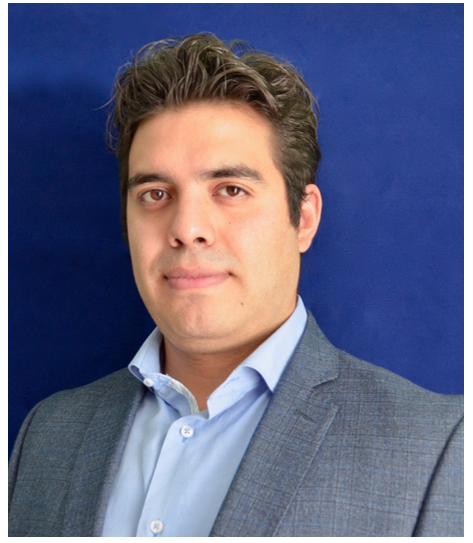
\includegraphics[width=250pt]{img/00-presentacion/arturo} \end{center}

\section*{Alcances del curso}\label{alcances-del-curso}
\addcontentsline{toc}{section}{Alcances del curso}

Al finalizar este curso, el participante será capaz de \ldots{}

Requisitos:

\begin{itemize}
\tightlist
\item
  Computadora con al menos 8Gb Ram
\item
  Instalar Git con versión XXX o superior
\item
  Instalar un IDE VSCode
\end{itemize}

\subsection*{Temario:}\label{temario}
\addcontentsline{toc}{subsection}{Temario:}

\section*{Duración y evaluación del curso}\label{duraciuxf3n-y-evaluaciuxf3n-del-curso}
\addcontentsline{toc}{section}{Duración y evaluación del curso}

\begin{itemize}
\item
  El programa tiene una duración de XX hrs.
\item
  Las clases serán impartidas los días sábado, de 9:00 am a 11:00 am
\item
  Serán asignados ejercicios que el participante deberá resolver entre una semana y otra.
\end{itemize}

\section*{Recursos y dinámica de clase}\label{recursos-y-dinuxe1mica-de-clase}
\addcontentsline{toc}{section}{Recursos y dinámica de clase}

En esta clase estaremos usando:

\begin{itemize}
\tightlist
\item
  Git
\item
  VSCode \href{https://code.visualstudio.com/download}{da click aquí si quieres descargar}
\item
  Zoom \href{https://us02web.zoom.us/j/5155440751?pwd=YzJCOGF0VnlZdlZlS0Fpc3MvZEhadz09}{Clases}

  \begin{itemize}
  \tightlist
  \item
    Pulgar arriba: Voy bien, estoy entendiendo!
  \item
    Pulgar abajo: Eso no quedó muy claro
  \item
    Mano arriba: Quiero participar/preguntar ó Ya estoy listo para iniciar
  \end{itemize}
\item
  \href{https://1drv.ms/f/s!AuOiA083gYHmhLdIesliXOiFEVnC7Q?e=NMcoy2}{One Drive}
\item
  Notas de clase \href{}{Revisame si quieres aprender}
\end{itemize}

\section*{Asesorías}\label{asesoruxedas}
\addcontentsline{toc}{section}{Asesorías}

Los profesores se encuentran en la mejor disposición de asistir las dudas de clase de todos los alumnos. El grupo de whatsapp ha sido creado para compartir información relevante al curso y exponer dudas y soluciones que puedan ser de interés de todo el grupo.

Los alumnos podrán hacer uso del canal de comunicación para externar sus dudas de clase durante el tiempo que dure el curso. Los profesores se comprometen a responder en el transcurso del día las preguntas realizadas que sean relevantes con la clase. Las respuestas se realizarán de lunes a viernes en un horario de 10:00am a 8:00pm.

\begin{infobox}{important}

\textbf{¡¡ AVISO !!}

\begin{itemize}
\item
  No se atenderán dudas que tengan que ver con otros proyectos o asignaciones laborales de los estudiantes en sus respectivos ambientes de trabajo.
\item
  Se invita a los estudiantes a que las dudas realizadas en clase sean relevantes a la clase y los ejemplos a resolver sean de interés para todo el alumnado.
\end{itemize}

\end{infobox}

\textbf{Nota:} En caso de requerir consultoría especializada o particular a un tema de interés, se deberá contactar al área administrativa para solicitar la cotización correspondiente al servicio correspondiente.

\chapter{Introducción del curso}\label{introducciuxf3n-del-curso}

\section{Objetivos del Curso}\label{objetivos-del-curso}

\emph{En esta sección, se menciona a grandes razgos el contenido del curso en general, por lo que todos los detalles se expondrán en sus respectivas secciones; no usaremos Git hasta la sección 2.}

\pandocbounded{
\includegraphics[keepaspectratio]{img/01_Intro/png-clipart-computer-icons-school-of-welcome-text-logo.png}}

Bienvenidos a este curso introductorio de Git, en este curso nos encaminaremos al dominio de una de las herramientas más útiles para todo desarrollador.

Git es un sistema de control de versiones,diseñado para manejar de todo, desde pequeños proyectos independientes hasta grandes y ambiciosos proyectos con rapidez y eficiencia. es una herramienta esencial para desarroladores de cualquier ámbito, ya que facilita la colaboración y el seguimiento de cambios en el código de manera organizada.

Tiene una clara orientación al código; te permite tener a dispocisión las versiones anteriores de cada proyecto en el que trabajes con el fin de tener una ``Linea del tiempo'' de tu proyecto que te permita ver los cambios que se han realizado a lo largo del tiempo.

\pandocbounded{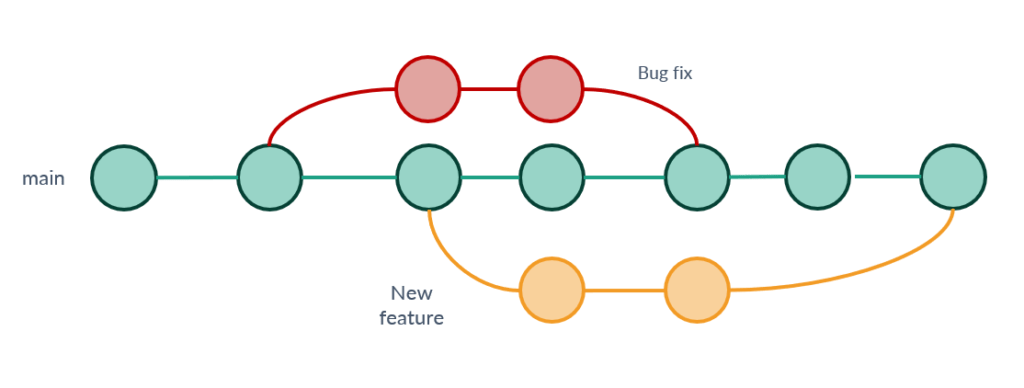
\includegraphics[keepaspectratio]{img/01_Intro/imagen-4-1024x388.png}}

Git, de manera automática (a menos que se encuentre un conflicto);

\begin{itemize}
\item
  Lee los archivos involucrados en el proyecto
\item
  Determina que cambios hubo en cada archivo actualizado
\item
  Une bloques de código de un mismo proyecto.
\end{itemize}

Un conflicto es que varios desarrolladores intentan hacer cambios distintos al mismo contendo, lo que hace que git no sepa cuales cambios guardar.

\pandocbounded{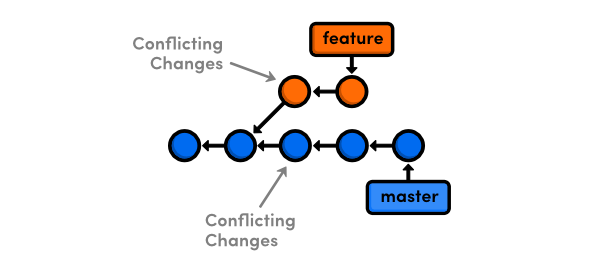
\includegraphics[keepaspectratio]{img/01_Intro/conflicts-1.png}}

Existen tecnicas para evitar conflictos, estas se verán dentro del curso.

El objetivo de este curso es que puedas:

\begin{itemize}
\item
  Administrar y organizar tu equipo de trabajo
\item
  Plantear y alcanzar metas en conjunto
\item
  Tener una visión general del repositorio de trabajo
\end{itemize}

En este curso no se utilizarán gestores con interfáz gráfica, ya que la mayoría de las características más nuevas de git no han sido implementadas en gestores visuales, dado que este tipo de gestores son de uso más básico. Por ello priorizaremos el uso de la consola / terminal del sistema operativo (En el caso de Windows se recomienda utilizar Git Bash) pero, para mayor comodidad, se hará uso de Visual Studio Code.

\pandocbounded{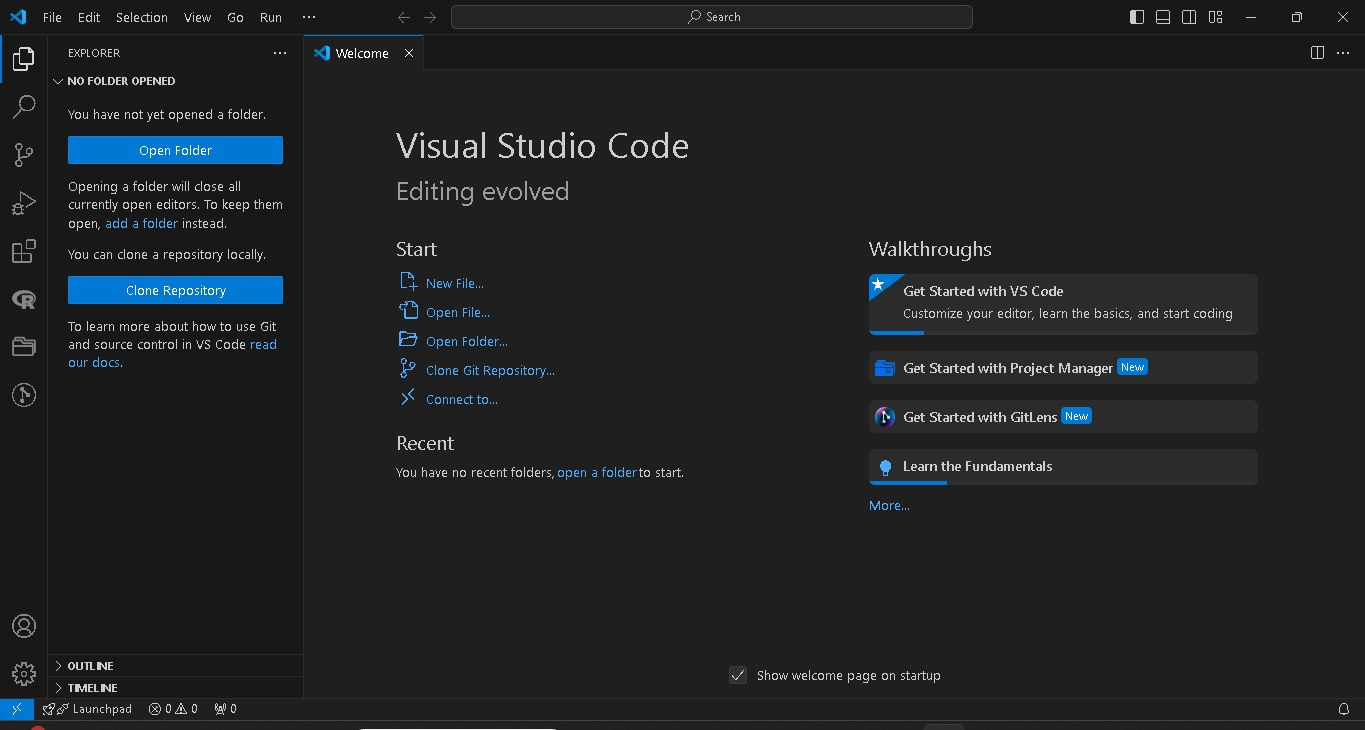
\includegraphics[keepaspectratio]{img/01_Intro/visual-studio-code.jpg}}

\textbf{Consejo:} Tener una librería (archivo de todos los comandos que veamos), será muy útil para repasar el contenido que vayamos viendo lo que reforzará sus conocimientos adquiridos en el curso.

\section{¿Cómo funciona el curso?}\label{cuxf3mo-funciona-el-curso}

El curso se dará en sesiones sincrónicas de aproximadamente 4 horas de duración, a través de zoom, en las que se explican los temas y se presentan ejemplos claros de cada lección para reforzar los conocimientos adquiridos en estas sesiones, contamos con:

\begin{itemize}
\item
  Tareas practicas
\item
  Material para ejercicios y prácticas
\end{itemize}

Para el curso se creará un grupo de WhatsApp en el que se encontrarán los instructores para que puedan expresar sus dudas o compartir material concerniente al curso, sobre todo fuera de las sesiones.

\section{Instalaciones}\label{instalaciones}

Antes de cualquier otra cosa debemos instalar tanto Git, como Visual Studio Code, para ello dejamos enlaces a las páginas oficiales de ambos programas.

Enlaces:

\begin{itemize}
\item
  \href{https://git-scm.com/downloads}{Git}
\item
  \href{https://code.visualstudio.com/download}{Visual Studio Code}
\end{itemize}

Respecto a la documentación, no recommendamos que la lean sin los conocimientos básicos de git, tras haber terminado el curso estarán familiarizados con el mismo lenguaje, lo que les permitirá comprender mejor el contenido de la propia documentación.

\chapter{Fundamentos de Git}\label{fundamentos-de-git}

A continuación, un par de recomendaciones para el resto del curso:

\begin{itemize}
\item
  Tomar nota de los comandos que se verán en el curso, así como de que hace y como funciona cada uno, de forma que ustedes mismos entiendan lo que hace un comando y en que casos se ocupa.
\item
  Constantemente revisar su lista de comandos, esto para que vayan repasando y se familiaricen con los mismos, es recomendable hacerlo antes de cada sesión para tener esos conocimientos frescos.
\end{itemize}

\section{Introducción a los fundamentos de Git}\label{introducciuxf3n-a-los-fundamentos-de-git}

Git es un sistema de control de versiones que, a diferencia de otros sistemas de control de versiones, almacena y maneja la información como un conjunto de copias instantáneas de un sistema de archivos miniatura.

La mayoría de las operaciones en Git solo necesitan archivos y recursos locales para funcionar, lo que lo hace muy rápido.

Git tiene tres estados principales en los que se pueden encontrar tus archivos:

\begin{itemize}
\item
  \textbf{Confirmado:} significa que los datos están almacenados de manera segura en tu base de datos local.
\item
  \textbf{Modificado:} significa que has modificado el archivo pero todavía no lo has confirmado a tu base de datos.
\item
  \textbf{Preparado:} significa que has marcado un archivo modificado en su versión actual para que vaya en tu próxima confirmación.
\end{itemize}

Esto nos lleva a las tres secciones principales de un proyecto de Git: El directorio de Git (Git directory), el directorio de trabajo (working directory), y el área de preparación (staging area).

\begin{itemize}
\item
  \textbf{El directorio de Git:} Es donde se almacenan los metadatos y la base de datos de objetos para tu proyecto.
\item
  \textbf{El directorio de trabajo:} Es una copia de una versión del proyecto. Estos archivos se sacan de la base de datos comprimida en el directorio de Git, y se colocan en disco para que los puedas usar o modificar.
\item
  \textbf{El área de preparación:} Es un archivo, generalmente contenido en tu directorio de Git, que almacena información acerca de lo que va a ir en tu próxima confirmación. A veces se le denomina índice (``index'').
\end{itemize}

Git está diseñado para gestionar proyectos de software y otros tipos de documentos de manera eficiente y colaborativa. Aquí están algunos conceptos fundamentales:

\begin{itemize}
\item
  \textbf{Repositorio:} Es un espacio donde Git almacena todos los archivos y carpetas que forman parte de tu proyecto.
\item
  \textbf{Clonar:} Es hacer una copia exacta de un repositorio remoto en tu máquina local.
\item
  \textbf{Status:} Muestra el estado actual de tu repositorio de Git, incluyendo cambios sin confirmar y archivos no rastreados.
\item
  \textbf{Commit:} Es un registro de cambios en el repositorio. Cada commit tiene un mensaje que describe los cambios realizados.
\item
  \textbf{Branch (Rama):} Es una versión paralela del código principal. Se utilizan para desarrollar funcionalidades nuevas sin afectar el código principal hasta que estén listas.
\item
  \textbf{Merge (Fusionar):} Es el proceso de combinar cambios de una rama a otra. Por ejemplo, fusionar una rama de funcionalidad en la rama principal (como \texttt{main} o \texttt{master}).
\item
  \textbf{Push (Subir)} y \textbf{Pull (Bajar):} \texttt{Push} se refiere a enviar cambios locales al repositorio remoto, mientras que \texttt{Pull} es obtener cambios del repositorio remoto a tu repositorio local.
\end{itemize}

\pandocbounded{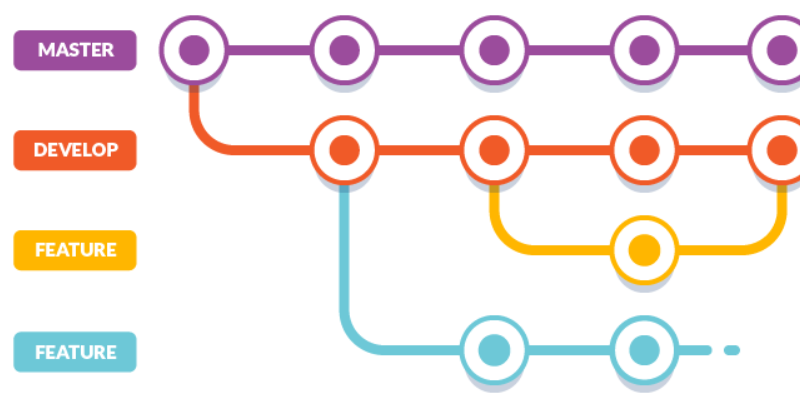
\includegraphics[keepaspectratio]{img/02_Fundamentos/SCV.png}}

\section{Importancia de Git}\label{importancia-de-git}

\textbf{¿Porqué es importante saber Git o cualquier otro sistema de control de versiones?}

Los sistemas de control de versiones (SCV), como lo es Git, son fundamentales en el desarrollo de software por varias razones clave:

\begin{itemize}
\item
  \textbf{Gestión de Historial:} Permiten mantener un registro detallado de todos los cambios realizados en el código y documentos del proyecto. Cada modificación se documenta con un mensaje descriptivo, lo que facilita la comprensión de la evolución del proyecto.
\item
  \textbf{Colaboración Eficiente:} Facilitan el trabajo en equipo al permitir que varios desarrolladores trabajen simultáneamente en diferentes aspectos del proyecto. Las ramas (branches) permiten trabajar en nuevas funcionalidades sin interferir con el código principal.
\item
  \textbf{Reversión y Recuperación:} Ofrecen la capacidad de revertir cambios no deseados o recuperar versiones anteriores del código en caso de errores o problemas inesperados.
\item
  \textbf{Experimentación Segura:} Las ramas permiten probar nuevas ideas de forma segura antes de integrarlas en el código principal, lo que ayuda a mantener la estabilidad del proyecto.
\item
  \textbf{Seguimiento de Responsabilidades:} Asignan responsabilidades claras al registrar quién realizó cada cambio y cuándo, lo que facilita la revisión y la resolución de problemas.
\end{itemize}

Es como en un videojuego donde tienes \textbf{puntos de control}, en el caso de Git serían los \textbf{commits}, a los que puedes volver si te encuentras en un problema y debes andar por otro camino o seguir una estrategia diferente.

\pandocbounded{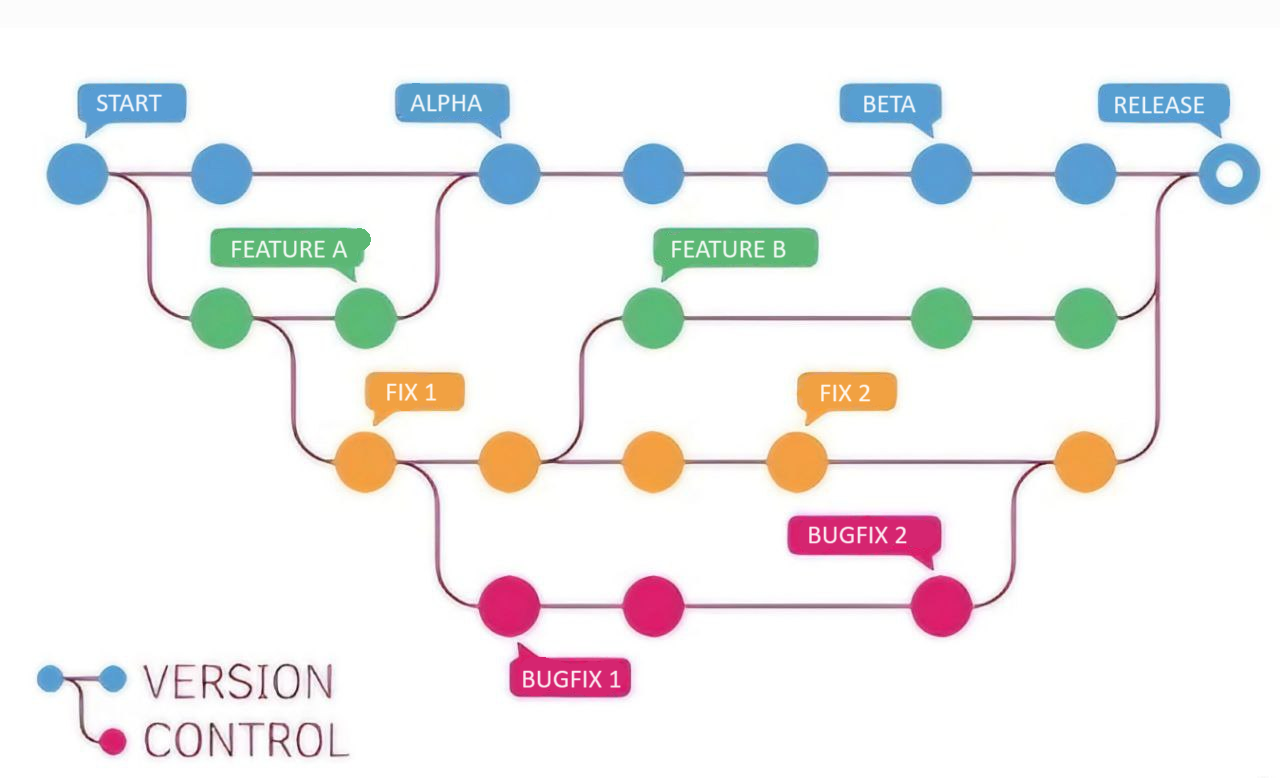
\includegraphics[keepaspectratio]{img/02_Fundamentos/version-control.png}}

En resumen, los SCV son esenciales para mantener la integridad, colaboración y evolución ordenada de los proyectos de software, mejorando la eficiencia y reduciendo el riesgo de errores en el desarrollo.

Existen distintos modelos de SCV, a continuación explicaremos 2 de los más implementados, veremos sus características y complementaremos con una analogía.

\begin{itemize}
\item
  \textbf{Repositorio Central}

  \pandocbounded{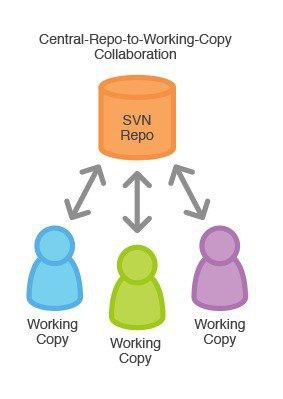
\includegraphics[keepaspectratio]{img/02_Fundamentos/repositorio-central.jpeg}}

  Es un modelo de control de versiones donde existe un único servidor central que contiene la versión principal del proyecto. Los desarrolladores envían sus cambios directamente a este servidor central.

  \textbf{Características:}

  \begin{itemize}
  \item
    \textbf{Centralizado:} Todos los desarrolladores envían y reciben cambios desde el mismo lugar.
  \item
    \textbf{Dependencia del servidor:} Requiere acceso constante al servidor central para realizar operaciones clave como commits y actualizaciones.
  \item
    \textbf{Historial único:} El historial completo del proyecto reside en el servidor central.
  \end{itemize}

  \textbf{Ejemplo:}

  Imagina que hay una Torre de los Vengadores \textbf{(Repositorio Central)} en Nueva York. Esta Torre es el cuartel general de los Vengadores y donde se almacenan todas las misiones y planes importantes \textbf{(código fuente)}. Todos los Vengadores \textbf{(desarrolladores)} tienen que ir a esta torre para obtener las misiones y para reportar los resultados de sus tareas.

  \begin{enumerate}
  \def\labelenumi{\arabic{enumi}.}
  \item
    \textbf{\emph{Obteniendo misiones} (Pulling)}: Cada Vengador \textbf{(desarrollador)} vuela a la Torre de los Vengadores \textbf{(repositorio central)} para obtener su misión \textbf{(código actual)}. Cuando alguien necesita una actualización, va directamente a la Torre.
  \item
    \textbf{\emph{Reportando misiones completadas} (Pushing)}: Una vez que el Vengador ha completado su misión \textbf{(hecho sus cambios)}, vuelve a la Torre para informar \textbf{(hacer push)} y actualizar el cuartel general con los resultados. Todos los demás Vengadores pueden ver esta actualización la próxima vez que vuelvan a la Torre.
  \end{enumerate}

  En este modelo, la Torre de los Vengadores es la única fuente de verdad y todos los Vengadores dependen de ella.
\item
  \textbf{Repositorio Distribuido}

  \pandocbounded{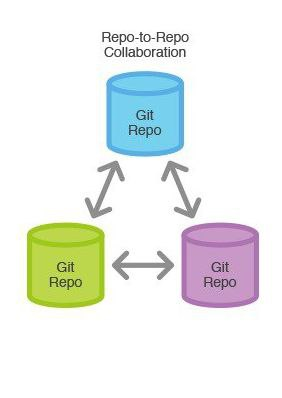
\includegraphics[keepaspectratio]{img/02_Fundamentos/repositorio-distribuido.jpeg}}

  En este modelo cada desarrollador tiene una copia completa del repositorio, incluyendo historial y ramas, en su máquina local. Los cambios se intercambian directamente entre repositorios locales o a través de uno central opcional.

  \textbf{Características:}

  \begin{itemize}
  \item
    \textbf{Descentralizado:} Cada desarrollador tiene su propio repositorio completo, lo que permite trabajar sin conexión a internet y facilita la colaboración.
  \item
    \textbf{Flexibilidad:} Los cambios pueden ser compartidos entre repositorios locales o a través de repositorios remotos.
  \item
    \textbf{Ramas y experimentación:} Permite a los desarrolladores trabajar en ramas independientes y experimentar sin afectar el repositorio principal hasta que estén listos.
  \end{itemize}

  \textbf{Ejemplo:}

  Ahora, imagina que el multiverso de Marvel está en plena acción, con diferentes versiones de los Vengadores en cada universo. Cada uno de estos equipos de Vengadores \textbf{(desarrolladores)} tiene su propia Torre \textbf{(su propio repositorio)} en su universo.

  \begin{enumerate}
  \def\labelenumi{\arabic{enumi}.}
  \item
    \textbf{\emph{Misiones propias} (Local Commits)}: En cada universo, los Vengadores tienen sus propias misiones que pueden completar de manera independiente, sin tener que volver a la Torre principal en Nueva York. Cada universo tiene su propia copia de las misiones \textbf{(repositorio completo)} y pueden hacer cambios sin necesidad de interactuar con otros universos.
  \item
    \textbf{\emph{Intercambio de misiones entre universos} (Push/Pull entre repositorios)}: A veces, los Vengadores de un universo pueden decidir compartir misiones o resultados con otro universo. Por ejemplo, los Vengadores de \emph{Tierra-616} podrían decidir que los Vengadores de \emph{Tierra-199999} necesitan saber algo que descubrieron. Entonces, envían esa misión o resultado \textbf{(push)} a la Torre de otro universo o piden recibir actualizaciones \textbf{(pull)} de ellos.
  \item
    \textbf{\emph{Sin Torre central única}}: No hay una \textbf{Torre central} a la que todos los Vengadores tengan que ir. Cada universo es autónomo y puede compartir información con otros universos según sea necesario.
  \end{enumerate}
\end{itemize}

La diferencia clave radica en la arquitectura y la forma en que se gestionan y comparten los cambios. Los repositorios centrales son más tradicionales y dependen de un servidor centralizado, mientras que los distribuidos ofrecen mayor flexibilidad, autonomía y capacidad de trabajo offline.

Git trabaja con el sistema de repositorio distribuido lo que permite que todo el equipo trabaje libremente sin depender de que el servidor central permanezca en condiciones de trabajo.

\pandocbounded{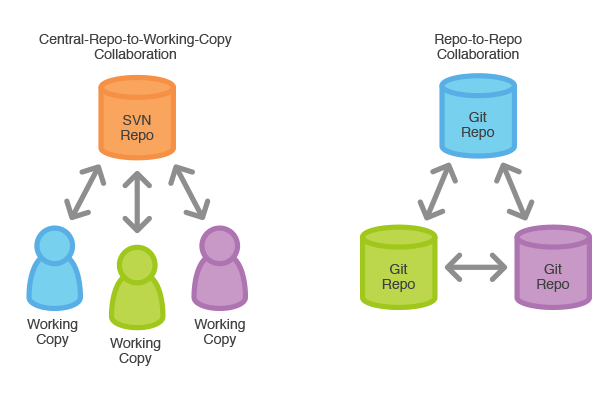
\includegraphics[keepaspectratio]{img/02_Fundamentos/svn-vs-git.png}}

\section{Configuración inicial de Git}\label{configuraciuxf3n-inicial-de-git}

Para comenzar vamos a configurar nuestro nombre de usuario, así como nuestro correo electrónico, estos van a servir para identificarnos y, más adelante, conectarnos con Github.

\begin{Shaded}
\begin{Highlighting}[]
\FunctionTok{git}\NormalTok{ config }\AttributeTok{{-}{-}global}\NormalTok{ user.name }\StringTok{"[Nombre de usuario]"}
\end{Highlighting}
\end{Shaded}

\begin{Shaded}
\begin{Highlighting}[]
\FunctionTok{git}\NormalTok{ config }\AttributeTok{{-}{-}global}\NormalTok{ user.email }\StringTok{"[Direccion de correo]"}
\end{Highlighting}
\end{Shaded}

El correo no necesariamnete debe estar registrado en Github, sin embargo, para trabajar con esta plataforma es recomendable usar el correo con el que te registraste o vas a registrar en Github, ya que tanto el nombre como el correo sirven para identificar al usuario.

Al iniciar un repositorio, Git crea una rama principal que generalmente es llamada \texttt{master} o \texttt{main}, Por diversas razones ultimamente esta segunda opción se ha vuelto la prferencia, por lo que vamos a establecer \texttt{main} como nombre por defecto de la rama principal:

\begin{Shaded}
\begin{Highlighting}[]
\FunctionTok{git}\NormalTok{ config }\AttributeTok{{-}{-}global}\NormalTok{ init.defaultBranch main}
\end{Highlighting}
\end{Shaded}

Con este comando se establece \texttt{main} como nombre por defecto de la rama principal para cualquier nuevo repositorio.

Si prefieres cambiar el nombre de la rama principal, o cualquier otra, puedes usar:

\begin{Shaded}
\begin{Highlighting}[]
\FunctionTok{git}\NormalTok{ branch }\AttributeTok{{-}m} \PreprocessorTok{[}\SpecialStringTok{actual}\PreprocessorTok{]} \PreprocessorTok{[}\SpecialStringTok{nuevo}\PreprocessorTok{]}
\end{Highlighting}
\end{Shaded}

Cambia el nombre \texttt{{[}actual{]}} de la rama por el \texttt{{[}nuevo{]}} en el repositorio actual sin alterar la configuración.

Para visualizar las configuraciones que tenemos en git, podemos utilizar el comando

\begin{Shaded}
\begin{Highlighting}[]
\FunctionTok{git}\NormalTok{ config }\AttributeTok{{-}{-}global} \AttributeTok{{-}e}
\end{Highlighting}
\end{Shaded}

\begin{Shaded}
\begin{Highlighting}[]
\ExtensionTok{[user]}
  \ExtensionTok{name}\NormalTok{ = Nombre de usuario}
  \ExtensionTok{email}\NormalTok{ = Direccion de correo}
\ExtensionTok{[init]}
  \ExtensionTok{defaultBranch}\NormalTok{ = main}
\end{Highlighting}
\end{Shaded}

Este comando abre el archivo de configuración global de Git en el editor de texto predeterminado para que puedas editarlo.

\section{Primeros comandos de Git}\label{primeros-comandos-de-git}

Para empezar vamos a abrir la terminal, en caso de Windows Git Bash, para presentar los primeros comandos.

\begin{Shaded}
\begin{Highlighting}[]
\FunctionTok{git} \AttributeTok{{-}{-}version}
\end{Highlighting}
\end{Shaded}

\begin{Shaded}
\begin{Highlighting}[]
\FunctionTok{git}\NormalTok{ version 2.47.0}
\end{Highlighting}
\end{Shaded}

Muestra la versión instalada de Git en tu sistema. En este caso contamos con la versión \texttt{2.47.0} de Git.

\begin{Shaded}
\begin{Highlighting}[]
\FunctionTok{git} \AttributeTok{{-}{-}help}
\end{Highlighting}
\end{Shaded}

\begin{Shaded}
\begin{Highlighting}[]
\ExtensionTok{usage:}\NormalTok{ git }\PreprocessorTok{[{-}{-}}\SpecialStringTok{version}\PreprocessorTok{]} \PreprocessorTok{[{-}{-}}\SpecialStringTok{help}\PreprocessorTok{]}\NormalTok{ [{-}C }\OperatorTok{\textless{}}\NormalTok{path}\OperatorTok{\textgreater{}}\NormalTok{] [{-}c }\OperatorTok{\textless{}}\NormalTok{name}\OperatorTok{\textgreater{}}\NormalTok{=}\OperatorTok{\textless{}}\NormalTok{value}\OperatorTok{\textgreater{}}\NormalTok{]}
           \ExtensionTok{[{-}{-}exec{-}path[=}\OperatorTok{\textless{}}\NormalTok{path}\OperatorTok{\textgreater{}}\NormalTok{]] }\PreprocessorTok{[{-}{-}}\SpecialStringTok{html}\PreprocessorTok{{-}}\SpecialStringTok{path}\PreprocessorTok{]} \PreprocessorTok{[{-}{-}}\SpecialStringTok{man}\PreprocessorTok{{-}}\SpecialStringTok{path}\PreprocessorTok{]} \PreprocessorTok{[{-}{-}}\SpecialStringTok{info}\PreprocessorTok{{-}}\SpecialStringTok{path}\PreprocessorTok{]}
           \ExtensionTok{[{-}p} \KeywordTok{|} \ExtensionTok{{-}{-}paginate} \KeywordTok{|} \ExtensionTok{{-}P} \KeywordTok{|} \ExtensionTok{{-}{-}no{-}pager]} \PreprocessorTok{[{-}{-}}\SpecialStringTok{no}\PreprocessorTok{{-}}\SpecialStringTok{replace}\PreprocessorTok{{-}}\SpecialStringTok{objects}\PreprocessorTok{]} \PreprocessorTok{[{-}{-}}\SpecialStringTok{bare}\PreprocessorTok{]}
           \ExtensionTok{[{-}{-}git{-}dir=}\OperatorTok{\textless{}}\NormalTok{path}\OperatorTok{\textgreater{}}\NormalTok{] [{-}{-}work{-}tree=}\OperatorTok{\textless{}}\NormalTok{path}\OperatorTok{\textgreater{}}\NormalTok{] [{-}{-}namespace=}\OperatorTok{\textless{}}\NormalTok{name}\OperatorTok{\textgreater{}}\NormalTok{]}
           \ExtensionTok{[{-}{-}super{-}prefix=}\OperatorTok{\textless{}}\NormalTok{path}\OperatorTok{\textgreater{}}\NormalTok{] [{-}{-}config{-}env=}\OperatorTok{\textless{}}\NormalTok{name}\OperatorTok{\textgreater{}}\NormalTok{=}\OperatorTok{\textless{}}\NormalTok{envvar}\OperatorTok{\textgreater{}}\NormalTok{]}
           \OperatorTok{\textless{}}\NormalTok{command}\OperatorTok{\textgreater{}} \ExtensionTok{[}\OperatorTok{\textless{}}\NormalTok{args}\OperatorTok{\textgreater{}}\NormalTok{]}

\ExtensionTok{These}\NormalTok{ are common Git commands used in various situations:}

\ExtensionTok{start}\NormalTok{ a working area }\ErrorTok{(}\ExtensionTok{see}\NormalTok{ also: git help tutorial}\KeywordTok{)}
   \ExtensionTok{clone}\NormalTok{     Clone a repository into a new directory}
   \ExtensionTok{init}\NormalTok{      Create an empty Git repository or reinitialize an existing one}

\ExtensionTok{work}\NormalTok{ on the current change }\ErrorTok{(}\ExtensionTok{see}\NormalTok{ also: git help everyday}\KeywordTok{)}
   \ExtensionTok{add}\NormalTok{       Add file contents to the index}
   \FunctionTok{mv}\NormalTok{        Move or rename a file, a directory, or a symlink}
   \ExtensionTok{restore}\NormalTok{   Restore working tree files}
   \FunctionTok{rm}\NormalTok{        Remove files from the working tree and from the index}

\ExtensionTok{examine}\NormalTok{ the history and state }\ErrorTok{(}\ExtensionTok{see}\NormalTok{ also: git help revisions}\KeywordTok{)}
   \ExtensionTok{bisect}\NormalTok{    Use binary search to find the commit that introduced a bug}
   \FunctionTok{diff}\NormalTok{      Show changes between commits, commit and working tree, etc}
   \FunctionTok{grep}\NormalTok{      Print lines matching a pattern}
   \ExtensionTok{log}\NormalTok{       Show commit logs}
   \ExtensionTok{show}\NormalTok{      Show various types of objects}
   \ExtensionTok{status}\NormalTok{    Show the working tree status}

\ExtensionTok{grow,}\NormalTok{ mark and tweak your common history}
   \ExtensionTok{branch}\NormalTok{    List, create, or delete branches}
   \ExtensionTok{commit}\NormalTok{    Record changes to the repository}
   \ExtensionTok{merge}\NormalTok{     Join two or more development histories together}
   \ExtensionTok{rebase}\NormalTok{    Reapply commits on top of another base tip}
   \ExtensionTok{reset}\NormalTok{     Reset current HEAD to the specified state}
   \ExtensionTok{switch}\NormalTok{    Switch branches}
   \ExtensionTok{tag}\NormalTok{       Create, list, delete or verify a tag object signed with GPG}

\ExtensionTok{collaborate} \ErrorTok{(}\ExtensionTok{see}\NormalTok{ also: git help workflows}\KeywordTok{)}
   \ExtensionTok{fetch}\NormalTok{     Download objects and refs from another repository}
   \ExtensionTok{pull}\NormalTok{      Fetch from and integrate with another repository or a local branch}
   \ExtensionTok{push}\NormalTok{      Update remote refs along with associated objects}

\StringTok{\textquotesingle{}git help {-}a\textquotesingle{}}\NormalTok{ and }\StringTok{\textquotesingle{}git help {-}g\textquotesingle{}}\NormalTok{ list available subcommands and some}
\ExtensionTok{concept}\NormalTok{ guides. See }\StringTok{\textquotesingle{}git help \textless{}command\textgreater{}\textquotesingle{}}\NormalTok{ or }\StringTok{\textquotesingle{}git help \textless{}concept\textgreater{}\textquotesingle{}}
\ExtensionTok{to}\NormalTok{ read about a specific subcommand or concept.}
\OperatorTok{\textless{}}\NormalTok{!{-}{-} }\ExtensionTok{See} \StringTok{\textquotesingle{}git help git\textquotesingle{}}\NormalTok{ for an overview of the system. }\AttributeTok{{-}{-}}\OperatorTok{\textgreater{}}
\end{Highlighting}
\end{Shaded}

Muestra una lista de comandos disponibles en Git junto con una breve descripción de cada uno y cómo usarlos.

\begin{Shaded}
\begin{Highlighting}[]
\FunctionTok{git} \AttributeTok{{-}{-}help}\NormalTok{ [nombre del comando]}
\end{Highlighting}
\end{Shaded}

Muestra la documentación detallada y las opciones disponibles para el comando especificado en Git.

\section{Primer Repositorio {[}Ejercicio{]}}\label{primer-repositorio-ejercicio}

Con el material \href{material/Demografia.zip}{Demografia} y en compañía de los instructores, van a crear su primer repositorio, para ello hay que acceder a la carpeta \texttt{Demografia}, una vez descomprimido el arcivo \texttt{Demografia.zip}.

En este ejercicio se van a presentar los siguientes comandos:

\begin{Shaded}
\begin{Highlighting}[]
\FunctionTok{git}\NormalTok{ init}
\end{Highlighting}
\end{Shaded}

\begin{Shaded}
\begin{Highlighting}[]
\ExtensionTok{Inicializado}\NormalTok{ repositorio Git vacío en /}\PreprocessorTok{[}\SpecialStringTok{path}\PreprocessorTok{]}\NormalTok{/Demografia/.git/}
\end{Highlighting}
\end{Shaded}

Este comando inicializa un nuevo repositorio de Git en el directorio actual \texttt{{[}Demografia{]}}, creando un subdirectorio \texttt{.git} con todos los archivos necesarios para el control de versiones.

\begin{Shaded}
\begin{Highlighting}[]
\FunctionTok{git}\NormalTok{ status}
\end{Highlighting}
\end{Shaded}

\begin{Shaded}
\begin{Highlighting}[]
\ExtensionTok{En}\NormalTok{ la rama main}

\ExtensionTok{No}\NormalTok{ hay commits todavía}

\ExtensionTok{no}\NormalTok{ hay nada para confirmar }\ErrorTok{(}\ExtensionTok{crea/copia}\NormalTok{ archivos y usa }\StringTok{"git add"}\NormalTok{ para hacerles seguimiento}\KeywordTok{)}
\end{Highlighting}
\end{Shaded}

El comando muestra el estado actual del repositorio, incluyendo los cambios en el área de preparación y los archivos modificados que no están preparados para el commit.

\begin{Shaded}
\begin{Highlighting}[]
\FunctionTok{git}\NormalTok{ add images}
\end{Highlighting}
\end{Shaded}

Añade la carpeta \texttt{images} al área de preparación para ser incliudo en el próximo commit, en caso de ser un directorio se agregan tolos los archivos y subdirectorios que contiene.

\begin{Shaded}
\begin{Highlighting}[]
\FunctionTok{git}\NormalTok{ add .}
\end{Highlighting}
\end{Shaded}

Agrega todos los archivos nuevos y modificados del directorio actual al área de preparación para el próximo commit.

\begin{Shaded}
\begin{Highlighting}[]
\FunctionTok{git}\NormalTok{ reset EDOMEX{-}demo.R}
\end{Highlighting}
\end{Shaded}

Deshace los cambios en \texttt{EDOMEX-demo.R}, en este caso no hay cambios pero el archivo no se guardará, retirándolo del área de preparación sin modificar el directorio de trabajo.

Si verificamos el estado del repositorio, veremos algo así:

\begin{Shaded}
\begin{Highlighting}[]
\FunctionTok{git}\NormalTok{ status}
\end{Highlighting}
\end{Shaded}

\begin{Shaded}
\begin{Highlighting}[]
\ExtensionTok{En}\NormalTok{ la rama main}

\ExtensionTok{No}\NormalTok{ hay commits todavía}

\ExtensionTok{Cambios}\NormalTok{ a ser confirmados:}
  \KeywordTok{(}\ExtensionTok{usa} \StringTok{"git rm {-}{-}cached \textless{}archivo\textgreater{}..."}\NormalTok{ para sacar del área de stage}\KeywordTok{)}
    \ExtensionTok{nuevos}\NormalTok{ archivos: Demografia.Rmd}
    \ExtensionTok{nuevos}\NormalTok{ archivos: Demografia.pdf}
    \ExtensionTok{nuevos}\NormalTok{ archivos: DistribucionNE{-}2010.xlsx}
    \ExtensionTok{nuevos}\NormalTok{ archivos: DistribucionNE{-}2020.xlsx}
    \ExtensionTok{nuevos}\NormalTok{ archivos: EDOMEX2010.Rda}
    \ExtensionTok{nuevos}\NormalTok{ archivos: EDOMEX2010.csv}
    \ExtensionTok{nuevos}\NormalTok{ archivos: EDOMEX2010M.Rda}
    \ExtensionTok{nuevos}\NormalTok{ archivos: EDOMEX2020.Rda}
    \ExtensionTok{nuevos}\NormalTok{ archivos: EDOMEX2020.csv}
    \ExtensionTok{nuevos}\NormalTok{ archivos: EDOMEX2020M.Rda}
    \ExtensionTok{nuevos}\NormalTok{ archivos: images/indice{-}masculinidad.png}
    \ExtensionTok{nuevos}\NormalTok{ archivos: images/piramide{-}EDOMEX{-}2010.png}
    \ExtensionTok{nuevos}\NormalTok{ archivos: images/piramide{-}EDOMEX{-}2020.png}

\ExtensionTok{Archivos}\NormalTok{ sin seguimiento:}
  \KeywordTok{(}\ExtensionTok{usa} \StringTok{"git add \textless{}archivo\textgreater{}..."}\NormalTok{ para incluirlo a lo que será confirmado}\KeywordTok{)}
    \ExtensionTok{EDOMEX{-}demo.R}
\end{Highlighting}
\end{Shaded}

\begin{Shaded}
\begin{Highlighting}[]
\FunctionTok{git}\NormalTok{ commit }\AttributeTok{{-}m} \StringTok{"commit inicial"}
\end{Highlighting}
\end{Shaded}

\begin{Shaded}
\begin{Highlighting}[]
\ExtensionTok{[main} \ErrorTok{(}\ExtensionTok{commit{-}raíz}\KeywordTok{)} \ExtensionTok{37fd5c8]}\NormalTok{ commit inicial}
 \ExtensionTok{13}\NormalTok{ files changed, 395 insertions}\ErrorTok{(}\ExtensionTok{+}\KeywordTok{)}
 \ExtensionTok{create}\NormalTok{ mode 100644 Demografia.Rmd}
 \ExtensionTok{create}\NormalTok{ mode 100644 Demografia.pdf}
 \ExtensionTok{create}\NormalTok{ mode 100755 DistribucionNE{-}2010.xlsx}
 \ExtensionTok{create}\NormalTok{ mode 100755 DistribucionNE{-}2020.xlsx}
 \ExtensionTok{create}\NormalTok{ mode 100644 EDOMEX2010.Rda}
 \ExtensionTok{create}\NormalTok{ mode 100755 EDOMEX2010.csv}
 \ExtensionTok{create}\NormalTok{ mode 100644 EDOMEX2010M.Rda}
 \ExtensionTok{create}\NormalTok{ mode 100644 EDOMEX2020.Rda}
 \ExtensionTok{create}\NormalTok{ mode 100644 EDOMEX2020.csv}
 \ExtensionTok{create}\NormalTok{ mode 100644 EDOMEX2020M.Rda}
 \ExtensionTok{create}\NormalTok{ mode 100644 images/indice{-}masculinidad.png}
 \ExtensionTok{create}\NormalTok{ mode 100644 images/piramide{-}EDOMEX{-}2010.png}
 \ExtensionTok{create}\NormalTok{ mode 100644 images/piramide{-}EDOMEX{-}2020.png}
\end{Highlighting}
\end{Shaded}

Realiza un commit con un mensaje descriptivo especificado en \texttt{"commit\ inicial"}, guardando los cambios realizados en el repositorio de Git.

Hasta esta parte del ejercicio creaste tu primer repositorio, conociste al área de preparación e hiciste tu primer commit.
Quizá ahora tengas una pregunta en mente.

\textbf{¿Para qué me sirve estar haciendo commit frecuetemente?}.\\
Supongamos que por un fallo se corrompieron los archivos en los que estabas trabajando, o que por error borraste algo que no debías; esta clase de sucesos ocurren con bastante frecuencia pero, con ayuda de Git, podrás recuperar tu información.

\begin{Shaded}
\begin{Highlighting}[]
\FunctionTok{git}\NormalTok{ checkout }\AttributeTok{{-}{-}}\NormalTok{ .}
\end{Highlighting}
\end{Shaded}

El comando \texttt{git\ checkout} tiene muchas funcionalidades, pero en particular \texttt{git\ checkout\ -\/-\ .} restaura todos los archivos en el directorio de trabajo a su estado más reciente en el repositorio (último commit), descartando los cambios no confirmados, permitiendo recuperar la información delo último commit realizado, pero esto \textbf{sólo con los archivos a los que Git les da seguimiento}, por lo que es una buena páctica hacer commit con cierta regularidad.

\begin{Shaded}
\begin{Highlighting}[]
\FunctionTok{git}\NormalTok{ log}
\end{Highlighting}
\end{Shaded}

\begin{Shaded}
\begin{Highlighting}[]
\ExtensionTok{commit}\NormalTok{ e4d9d8e7b9367137765f42870a06e29d295a7434 }\ErrorTok{(}\ExtensionTok{HEAD} \AttributeTok{{-}}\OperatorTok{\textgreater{}}\NormalTok{ main}\KeywordTok{)}
\ExtensionTok{Author:}\NormalTok{ [Nombre de usuario] }\OperatorTok{\textless{}}\NormalTok{[Direccion de correo]}\OperatorTok{\textgreater{}}
\ExtensionTok{Date:}\NormalTok{   Mon Jul 8 21:55:45 2024 }\AttributeTok{{-}0600}

    \ExtensionTok{commit}\NormalTok{ inicial}
\end{Highlighting}
\end{Shaded}

Muestra el historial de commits del repositorio, incluyendo mensajes, autores y fechas, la clave alfanumérica que aparece al principio de cada commit es el hash con el que Git regitra ese commit, cada clave es distinta y le corresponde una única instantanea (commit).
Este comando muestra mucha información que realmente entorpece la visualización, pero hay maneras de mejorar la forma en que se presenta esta información.

\begin{Shaded}
\begin{Highlighting}[]
\FunctionTok{git}\NormalTok{ log }\AttributeTok{{-}{-}oneline}
\end{Highlighting}
\end{Shaded}

\begin{Shaded}
\begin{Highlighting}[]
\ExtensionTok{e4d9d8e} \ErrorTok{(}\ExtensionTok{HEAD} \AttributeTok{{-}}\OperatorTok{\textgreater{}}\NormalTok{ main}\KeywordTok{)} \ExtensionTok{commit}\NormalTok{ inicial}
\end{Highlighting}
\end{Shaded}

Muestra una forma reducida del hash de cada commit seguido de su mensaje de identificación.\\
Cabe aclarar que la palabra \texttt{HEAD} marca al último commit realizado y que \texttt{(HEAD\ -\textgreater{}\ main)} indica que dicho commit se realizó en la rama \texttt{main}.

\section{Distintas maneras de agregar elementos al Stage}\label{distintas-maneras-de-agregar-elementos-al-stage}

Ya sabemos que con \texttt{git\ add} podemos agregar uno por uno los elementos que deseamos al Stage (área de preparación), y que con \texttt{git\ add\ .} podemos agregar todos los archivos disponibles, pero imagina que modificaste muchos archivos, pero no quieres agregalos todos y hacerlo de uno en uno sería muy tardado.\\
Puedes agregar archivos con el mismo formata ubicados en el mismo directorio utilizando:

\begin{Shaded}
\begin{Highlighting}[]
\FunctionTok{git}\NormalTok{ add }\PreprocessorTok{*}\NormalTok{.}\PreprocessorTok{[}\SpecialStringTok{formato}\PreprocessorTok{]}
\end{Highlighting}
\end{Shaded}

Agrega al Stage todos los archivos \texttt{.{[}formato{]}} que se encuentren en el directorio actual, pero no hará nada con los archivos que se encuentren en un subdirectorio.

\begin{Shaded}
\begin{Highlighting}[]
\FunctionTok{git}\NormalTok{ add }\PreprocessorTok{[}\SpecialStringTok{subdirectorio}\PreprocessorTok{]}\NormalTok{/}\PreprocessorTok{*}\NormalTok{.}\PreprocessorTok{[}\SpecialStringTok{formato}\PreprocessorTok{]}
\end{Highlighting}
\end{Shaded}

Este comando agrega los archivos \texttt{.{[}formato{]}} dentro de \texttt{{[}subdirectorio{]}/} al Stage.

\begin{Shaded}
\begin{Highlighting}[]
\FunctionTok{git}\NormalTok{ add }\PreprocessorTok{[}\SpecialStringTok{subdirectorio}\PreprocessorTok{]}\NormalTok{/}
\end{Highlighting}
\end{Shaded}

Agrega todos los archivos modificados del \texttt{{[}subdirectorio{]}}.

\textbf{Nota:}

Git de manera automática ignora los directorios vacíos por lo que, si no tienes cuidado, puede ignorar un fichero importante y llegar a romper tu proyecto, para evitarlo se suele agregar un archivo llamado \texttt{.gitkeep} a las carpetas vacías un archivo especial para que git reconozca que debe hacerles seguimiento.

De esta manera puedes organizar más facilmente los elementos modificados.

\section{Repaso}\label{repaso}

Ahora un breve repaso de los comandos que hemos visto hasta ahora.

\begin{Shaded}
\begin{Highlighting}[]
\FunctionTok{git}\NormalTok{ config }\AttributeTok{{-}{-}global}\NormalTok{ user.name }\StringTok{"[Nombre de usuario]"}
\end{Highlighting}
\end{Shaded}

Configura el nombre de usuario global para todos los repositorios de Git en tu sistema.

\begin{Shaded}
\begin{Highlighting}[]
\FunctionTok{git}\NormalTok{ config }\AttributeTok{{-}{-}global}\NormalTok{ user.email }\StringTok{"[Direccion de correo]"}
\end{Highlighting}
\end{Shaded}

Configura el correo electrónico global para todos los repositorios de Git en tu sistema.

\begin{Shaded}
\begin{Highlighting}[]
\FunctionTok{git}\NormalTok{ config }\AttributeTok{{-}{-}global}\NormalTok{ init.defaultBranch main}
\end{Highlighting}
\end{Shaded}

Con este comando se establece \texttt{main} como nombre por defecto de la rama principal para cualquier nuevo repositorio.

\begin{Shaded}
\begin{Highlighting}[]
\FunctionTok{git}\NormalTok{ branch }\AttributeTok{{-}m} \PreprocessorTok{[}\SpecialStringTok{actual}\PreprocessorTok{]} \PreprocessorTok{[}\SpecialStringTok{nuevo}\PreprocessorTok{]}
\end{Highlighting}
\end{Shaded}

Cambia el nombre \texttt{{[}actual{]}} de la rama por el \texttt{{[}nuevo{]}}.

\begin{Shaded}
\begin{Highlighting}[]
\FunctionTok{git}\NormalTok{ config }\AttributeTok{{-}{-}global} \AttributeTok{{-}e}
\end{Highlighting}
\end{Shaded}

Abre el archivo de configuración global de Git en tu editor de texto predeterminado para que puedas editarlo.

\begin{Shaded}
\begin{Highlighting}[]
\FunctionTok{git} \AttributeTok{{-}{-}version}
\end{Highlighting}
\end{Shaded}

Muestra la versión instalada de Git en tu sistema

\begin{Shaded}
\begin{Highlighting}[]
\FunctionTok{git} \AttributeTok{{-}{-}help}
\end{Highlighting}
\end{Shaded}

Muestra una lista de comandos disponibles en Git junto con una breve descripción de cada uno y cómo usarlos.

\begin{Shaded}
\begin{Highlighting}[]
\FunctionTok{git} \AttributeTok{{-}{-}help}\NormalTok{ [nombre del comando]}
\end{Highlighting}
\end{Shaded}

Muestra la documentación detallada y las opciones disponibles para el comando especificado en Git.

\begin{Shaded}
\begin{Highlighting}[]
\FunctionTok{git}\NormalTok{ init}
\end{Highlighting}
\end{Shaded}

Este comando inicializa un nuevo repositorio de Git en el directorio actual.

\begin{Shaded}
\begin{Highlighting}[]
\FunctionTok{git}\NormalTok{ status}
\end{Highlighting}
\end{Shaded}

Muestra el estado actual del repositorio, incluyendo los cambios en el área de preparación y los archivos modificados que no están preparados para el commit.

\begin{Shaded}
\begin{Highlighting}[]
\FunctionTok{git}\NormalTok{ add}
\end{Highlighting}
\end{Shaded}

Añade archivos al área de preparación para ser incluidos en el próximo commit.

\begin{Shaded}
\begin{Highlighting}[]
\FunctionTok{git}\NormalTok{ add .}
\end{Highlighting}
\end{Shaded}

Agrega todos los archivos nuevos y modificados del directorio actual al área de preparación para el próximo commit.

\begin{Shaded}
\begin{Highlighting}[]
\FunctionTok{git}\NormalTok{ reset }\PreprocessorTok{[}\SpecialStringTok{archivo}\PreprocessorTok{]}
\end{Highlighting}
\end{Shaded}

Deshace los cambios en el archivo especificado, retirándolo del área de preparación sin modificar el directorio de trabajo.

\begin{Shaded}
\begin{Highlighting}[]
\FunctionTok{git}\NormalTok{ commit }\AttributeTok{{-}m} \StringTok{"nombre del commit"}
\end{Highlighting}
\end{Shaded}

Realiza un commit con un mensaje descriptivo especificado, guardando los cambios realizados en el repositorio de Git.

\begin{Shaded}
\begin{Highlighting}[]
\FunctionTok{git}\NormalTok{ checkout }\AttributeTok{{-}{-}}\NormalTok{ .}
\end{Highlighting}
\end{Shaded}

Restaura todos los archivos en el directorio de trabajo a su estado más reciente en el repositorio (último commit), descartando los cambios no confirmados.

\begin{Shaded}
\begin{Highlighting}[]
\FunctionTok{git}\NormalTok{ log}
\end{Highlighting}
\end{Shaded}

Muestra el historial de commits del repositorio, incluyendo mensajes, autores y fechas.

\begin{Shaded}
\begin{Highlighting}[]
\FunctionTok{git}\NormalTok{ add }\PreprocessorTok{*}\NormalTok{.}\PreprocessorTok{[}\SpecialStringTok{formato}\PreprocessorTok{]}
\end{Highlighting}
\end{Shaded}

Agrega al Stage todos los archivos \texttt{.{[}formato{]}} que se encuentren en el directorio actual.

\begin{Shaded}
\begin{Highlighting}[]
\FunctionTok{git}\NormalTok{ add }\PreprocessorTok{[}\SpecialStringTok{subdirectorio}\PreprocessorTok{]}\NormalTok{/}\PreprocessorTok{*}\NormalTok{.}\PreprocessorTok{[}\SpecialStringTok{formato}\PreprocessorTok{]}
\end{Highlighting}
\end{Shaded}

Este comando agrega los archivos \texttt{.{[}formato{]}} dentro de \texttt{{[}subdirectorio{]}/} al Stage.

\begin{Shaded}
\begin{Highlighting}[]
\FunctionTok{git}\NormalTok{ add }\PreprocessorTok{[}\SpecialStringTok{subdirectorio}\PreprocessorTok{]}\NormalTok{/}
\end{Highlighting}
\end{Shaded}

Agrega todos los archivos modificados del \texttt{{[}subdirectorio{]}}.

\section{Alias}\label{alias}

Ya conocen los comandos más básicos de Git y seguro han notado que muchos muestran información que generalmente no necesitamos, la gran mayoría de comandos en Git cuentan con etiquetas que permiten mostrar la información de manera distinta a como se hace normalmente pero, como se imaginarán, mejorar la visualización de la información hace que los comandos se extiendan mucho; por ello ahora aprenderán a crear sus propios alias.\\
Un alias de Git es un atajo personalizado que se configura para simplificar y acortar comandos de Git frecuentemente usados.

Para crear tu propio alias utiliza:

\begin{Shaded}
\begin{Highlighting}[]
\FunctionTok{git}\NormalTok{ config }\AttributeTok{{-}{-}global}\NormalTok{ alias.}\PreprocessorTok{[}\SpecialStringTok{alias}\PreprocessorTok{]} \StringTok{"[Comando]"}
\end{Highlighting}
\end{Shaded}

Establece un alias de manera que \texttt{git\ {[}alias{]}} hará lo mismo que \texttt{git\ "{[}comando{]}"}

Así pueden crear tus propios alias para facilitarse el trabajo.

Un ejemplo muy útil sería:

\begin{Shaded}
\begin{Highlighting}[]
\FunctionTok{git}\NormalTok{ config }\AttributeTok{{-}{-}global}\NormalTok{ alias.s }\StringTok{"status {-}s {-}b"}
\end{Highlighting}
\end{Shaded}

Veamos el cambio, la salida de \texttt{status}

\begin{Shaded}
\begin{Highlighting}[]
\FunctionTok{git}\NormalTok{ status}
\end{Highlighting}
\end{Shaded}

\begin{Shaded}
\begin{Highlighting}[]
\ExtensionTok{En}\NormalTok{ la rama main}
\ExtensionTok{Archivos}\NormalTok{ sin seguimiento:}
  \KeywordTok{(}\ExtensionTok{usa} \StringTok{"git add \textless{}archivo\textgreater{}..."}\NormalTok{ para incluirlo a lo que será confirmado}\KeywordTok{)}
    \ExtensionTok{EDOMEX{-}demo.R}

\ExtensionTok{no}\NormalTok{ hay nada agregado al commit pero hay archivos sin seguimiento presentes }\ErrorTok{(}\ExtensionTok{usa} \StringTok{"git add"}\NormalTok{ para hacerles seguimiento}\KeywordTok{)}
\end{Highlighting}
\end{Shaded}

La salida de \texttt{s}

\begin{Shaded}
\begin{Highlighting}[]
\FunctionTok{git}\NormalTok{ s}
\end{Highlighting}
\end{Shaded}

\begin{Shaded}
\begin{Highlighting}[]
\CommentTok{\#\# main}
\ExtensionTok{??}\NormalTok{ EDOMEX{-}demo.R}
\end{Highlighting}
\end{Shaded}

Como pueden ver, el uso de alias es muy útil, sobre todo con comandos que se usan repetidamente.

Por último una recomendación de \texttt{alias} que será muy útil en adelante:

\begin{Shaded}
\begin{Highlighting}[]
\FunctionTok{git}\NormalTok{ config }\AttributeTok{{-}{-}global}\NormalTok{ alias.lg }\StringTok{"log {-}{-}graph {-}{-}abbrev{-}commit {-}{-}decorate {-}{-}format=format:\textquotesingle{}\%C(bold blue)\%h\%C(reset) {-} \%C(bold green)(\%ar)\%C(reset) \%C(white)\%s\%C(reset) \%C(dim white){-} \%an\%C(reset)\%C(bold yellow)\%d\%C(reset)\textquotesingle{} {-}{-}all"}
\end{Highlighting}
\end{Shaded}

Con este alias se mostrarán los registros de un repositorio de manera resumida y organizada, de forma que será más facil identificar la información.

\chapter{Los cambios en Git}\label{los-cambios-en-git}

\section{Cambios en los archivos}\label{cambios-en-los-archivos}

Cuando acabas de editar un archivo y quieres ver con claridad las diferencias entre las ``versiones'', puedes hacerlo de varias formas, como hacer copia del ``original'' o ir revirtiendo los cambios poco a poco, pero tener toda la información disponible hace que fácilmente se pierda de vista lo que uno busca;
git puede mostrarte, de manera organizada, unicamente los cambios que hay entre las dos versiones que quieres comparar de un archivo, lo que facilita bastante distinguir los cambios efectuados.

En esta ocación presentaremos un comando que nos ayudará a distinguir los cambios realizados en un archivo.

\begin{Shaded}
\begin{Highlighting}[]
\FunctionTok{git}\NormalTok{ diff}
\end{Highlighting}
\end{Shaded}

\begin{Shaded}
\begin{Highlighting}[]
\FunctionTok{diff} \AttributeTok{{-}{-}git}\NormalTok{ a/Demografia.Rmd b/Demografia.Rmd}
\ExtensionTok{index}\NormalTok{ 0d2f647..090d477 100644}
\ExtensionTok{{-}{-}{-}}\NormalTok{ a/Demografia.Rmd}
\ExtensionTok{+++}\NormalTok{ b/Demografia.Rmd}
\ExtensionTok{@@} \AttributeTok{{-}134,10}\NormalTok{ +134,10 @@ }\VariableTok{$p\_f}\NormalTok{ = p\_i }\DataTypeTok{\textbackslash{}c}\NormalTok{dot e \^{} \{r }\DataTypeTok{\textbackslash{}c}\NormalTok{dot h\}$}
 
 \ExtensionTok{Donde:}
 
\ExtensionTok{{-}{-}}   \VariableTok{$p\_f}\NormalTok{$ es la población final}
\ExtensionTok{{-}{-}}   \VariableTok{$p\_i}\NormalTok{$ es la población inicial}
\ExtensionTok{{-}{-}}   \VariableTok{$r}\NormalTok{$ es la tasa de crecimiento}
\ExtensionTok{{-}{-}}   \VariableTok{$h}\NormalTok{$ es el tiempo de crecimiento}
\ExtensionTok{+*}   \VariableTok{$p\_f}\NormalTok{$ es la población final}
\ExtensionTok{+*}   \VariableTok{$p\_i}\NormalTok{$ es la población inicial}
\ExtensionTok{+*}   \VariableTok{$r}\NormalTok{$ es la tasa de crecimiento}
\ExtensionTok{+*}   \VariableTok{$h}\NormalTok{$ es el tiempo de crecimiento}
\end{Highlighting}
\end{Shaded}

Muestra las diferencias no confirmadas entre el directorio de trabajo y el último commit realizado. En la salida podemos notar que hay líneas que comienzan con \texttt{+} y \texttt{-}, estos cimbolos nos indican los cambios que presenta el archivo en el que se está trabajando respecto al último registro realizado.\\
\texttt{+{[}contenido{]}} Indica que se agregó \texttt{{[}contenido{]}} al archivo en cuestión, mientras que
\texttt{-{[}contenido{]}} Indica que \texttt{{[}contenido{]}} fue removido delarchivo, preo solo muestra cambios en archivos que ya tienen seguimiento y no reconoce los cambios que se encuentran en el stage. Las líneas que no cuentan con estos marcadores no han sido modificadas.

\begin{Shaded}
\begin{Highlighting}[]
\FunctionTok{git}\NormalTok{ diff }\AttributeTok{{-}{-}staged}
\end{Highlighting}
\end{Shaded}

\begin{Shaded}
\begin{Highlighting}[]
\FunctionTok{diff} \AttributeTok{{-}{-}git}\NormalTok{ a/Demografia.Rmd b/Demografia.Rmd}
\ExtensionTok{index}\NormalTok{ 0d2f647..090d477 100644}
\ExtensionTok{{-}{-}{-}}\NormalTok{ a/Demografia.Rmd}
\ExtensionTok{+++}\NormalTok{ b/Demografia.Rmd}
\ExtensionTok{@@} \AttributeTok{{-}134,10}\NormalTok{ +134,10 @@ }\VariableTok{$p\_f}\NormalTok{ = p\_i }\DataTypeTok{\textbackslash{}c}\NormalTok{dot e \^{} \{r }\DataTypeTok{\textbackslash{}c}\NormalTok{dot h\}$}
 
 \ExtensionTok{Donde:}
 
\ExtensionTok{{-}{-}}   \VariableTok{$p\_f}\NormalTok{$ es la población final}
\ExtensionTok{{-}{-}}   \VariableTok{$p\_i}\NormalTok{$ es la población inicial}
\ExtensionTok{{-}{-}}   \VariableTok{$r}\NormalTok{$ es la tasa de crecimiento}
\ExtensionTok{{-}{-}}   \VariableTok{$h}\NormalTok{$ es el tiempo de crecimiento}
\ExtensionTok{+*}   \VariableTok{$p\_f}\NormalTok{$ es la población final}
\ExtensionTok{+*}   \VariableTok{$p\_i}\NormalTok{$ es la población inicial}
\ExtensionTok{+*}   \VariableTok{$r}\NormalTok{$ es la tasa de crecimiento}
\ExtensionTok{+*}   \VariableTok{$h}\NormalTok{$ es el tiempo de crecimiento}
\end{Highlighting}
\end{Shaded}

Muestra las diferencias presentes en los elementos que se encuentran en el área de preparación de la misma manera que \texttt{git\ diff}.

\section{Correción de commits}\label{correciuxf3n-de-commits}

En ocaciones, por algún descuido, hacemos un commit con un mensaje incompleto, mal escrito o simplemente distinto a lo que buscamos presentar, pero no hay de que alarmarse, este mensaje se puede corregir de manera sencilla.

\begin{Shaded}
\begin{Highlighting}[]
\FunctionTok{git}\NormalTok{ commit }\AttributeTok{{-}{-}amend} \AttributeTok{{-}m} \StringTok{"[correccion]"}
\end{Highlighting}
\end{Shaded}

\begin{Shaded}
\begin{Highlighting}[]
\ExtensionTok{[main}\NormalTok{ 9d520f3] }\PreprocessorTok{[}\SpecialStringTok{correccion}\PreprocessorTok{]}
 \ExtensionTok{Date:}\NormalTok{ Thu Jul 11 18:21:25 2024 }\AttributeTok{{-}0600}
 \ExtensionTok{1}\NormalTok{ file changed, 5 insertions}\ErrorTok{(}\ExtensionTok{+}\KeywordTok{)}
\end{Highlighting}
\end{Shaded}

Este comando permite cambiar el mensaje del \textbf{último commit} registrado por \texttt{{[}correccion{]}}.

Tambien ocurre que hicimos una confirmación que puede considererse incompleta, aunque sencillamente podrías hacer otro commit con los cambios restantes, Git ofrece la opción de restaurar el commit deseado para continuar trabajando sobre él.

\begin{Shaded}
\begin{Highlighting}[]
\FunctionTok{git}\NormalTok{ reset }\AttributeTok{{-}{-}soft}\NormalTok{ HEAD\^{}}
\end{Highlighting}
\end{Shaded}

Deshace el último commit, manteniendo los cambios en el área de preparación.
Puedes sustituir \texttt{HEAD\^{}} por el hash correspondiente al último commit, incluso puedes hacerlo con cualquier otro commit, pero es más simple dejarlo así.

\chapter{Repositorio nuevo}\label{repositorio-nuevo}

En este capítulo vamos a simular distintos escenarios en los que nos podemos encontrar al desarrollar un proyecto;
Vamos a trabajar ahora con la carpeta \texttt{material-marvel}, que se proporcionará por los instructores, y pondremos en practica los conocimientos adquiridos hasta ahora a la vez que profundizamos en las distintas opciones que nos proporciona la herramienta Git.
Con ese propósito vamos a seguir una narrativa en la cual nos encontramos desarrollando un proyecto llamado números.

\section{Preparación de repositorio}\label{preparaciuxf3n-de-repositorio}

Primero vamos a preparar el repositorio y haremos que Git rastreé los cambios relalizados en el proyecto.

\begin{enumerate}
\def\labelenumi{\arabic{enumi}.}
\tightlist
\item
  Desde la terminal, nos colocamos en la ubicación de la carpeta \texttt{material-marvel/} e inicializamos un repositorio de Git con
\end{enumerate}

\begin{Shaded}
\begin{Highlighting}[]
\FunctionTok{git}\NormalTok{ init}
\end{Highlighting}
\end{Shaded}

\begin{Shaded}
\begin{Highlighting}[]
\ExtensionTok{Inicializado}\NormalTok{ repositorio Git vacío en }\PreprocessorTok{[}\SpecialStringTok{path}\PreprocessorTok{]}\NormalTok{/material{-}marvel/.git/}
\end{Highlighting}
\end{Shaded}

\begin{enumerate}
\def\labelenumi{\arabic{enumi}.}
\setcounter{enumi}{1}
\tightlist
\item
  Uno por uno, vamos a registrar los archivos: \texttt{README.md}, \texttt{descripciones.md}, \texttt{origenes.md}, \texttt{debilidades.md} y el directorio \texttt{misiones/} (haciendo commit); recuerde que debes llevarlos al Satage con
\end{enumerate}

\begin{Shaded}
\begin{Highlighting}[]
\FunctionTok{git}\NormalTok{ add }\PreprocessorTok{[}\SpecialStringTok{elemento}\PreprocessorTok{]}
\end{Highlighting}
\end{Shaded}

para luego poder registrarlos con un mensaje a traves de

\begin{Shaded}
\begin{Highlighting}[]
\FunctionTok{git}\NormalTok{ commit }\AttributeTok{{-}m} \StringTok{"[elemento] agregado"}
\end{Highlighting}
\end{Shaded}

\begin{Shaded}
\begin{Highlighting}[]
\ExtensionTok{[main} \ErrorTok{(}\ExtensionTok{commit{-}raíz}\KeywordTok{)} \ExtensionTok{ac02fe0]} \PreprocessorTok{[}\SpecialStringTok{elemento}\PreprocessorTok{]}\NormalTok{ agregado}
 \ExtensionTok{1}\NormalTok{ file changed, 17 insertions}\ErrorTok{(}\ExtensionTok{+}\KeywordTok{)}
 \ExtensionTok{create}\NormalTok{ mode 100644 }\PreprocessorTok{[}\SpecialStringTok{elemento}\PreprocessorTok{]}
\end{Highlighting}
\end{Shaded}

\begin{enumerate}
\def\labelenumi{\arabic{enumi}.}
\setcounter{enumi}{2}
\tightlist
\item
  Vamos a cambiar el mensaje de registro que hicimos al guardar el directorio \texttt{misiones/}, para ello usaremos
\end{enumerate}

\begin{Shaded}
\begin{Highlighting}[]
\FunctionTok{git}\NormalTok{ commit }\AttributeTok{{-}{-}amend}
\end{Highlighting}
\end{Shaded}

\begin{Shaded}
\begin{Highlighting}[]
\ExtensionTok{misiones/}\NormalTok{ agregado}

\CommentTok{\# Please enter the commit message for your changes. Lines starting}
\CommentTok{\# with \textquotesingle{}\#\textquotesingle{} will be ignored, and an empty message aborts the commit.}
\CommentTok{\#}
\CommentTok{\# Fecha:     Wed Jan 15 16:29:04 2025 {-}0600}
\CommentTok{\#}
\CommentTok{\# En la rama main}
\CommentTok{\# Cambios a ser confirmados:}
\CommentTok{\#       nuevos archivos: misiones/black\_widow.md}
\CommentTok{\#       nuevos archivos: misiones/hulk.md}
\CommentTok{\#       nuevos archivos: misiones/iron\_man.md}
\CommentTok{\#       nuevos archivos: misiones/spider\_man.md}
\CommentTok{\#       nuevos archivos: misiones/thor.md}
\CommentTok{\#}
\end{Highlighting}
\end{Shaded}

Este comando abrirá el editor de texto por defecto de cada equipo para mostrar un archivo de registro, el cual vamos a editar de la siguiente manera:
La primera línea, donde se encuentra escrito \texttt{misiones/\ agregado}, cambiaremos ese mensaje por:

\begin{Shaded}
\begin{Highlighting}[]
\ExtensionTok{misiones/}\NormalTok{ agregado }\AttributeTok{{-}}\OperatorTok{\textgreater{}}\NormalTok{ misiones de los heroes: iron man, thor, hulk, black widow y spider man.}
\end{Highlighting}
\end{Shaded}

Y guardemos los cambios en el archivo de registro.

Con los registros realizados hasta ahora, tomando en cuenta que se suguió la recomendación de \texttt{alias} presentada al final del Capítulo 2, usando \texttt{git\ lg} deberiamos tener una salida como la que sigue

\begin{Shaded}
\begin{Highlighting}[]
\FunctionTok{git}\NormalTok{ lg}
\end{Highlighting}
\end{Shaded}

\begin{Shaded}
\begin{Highlighting}[]
\ExtensionTok{*}\NormalTok{ a2427e8 }\AttributeTok{{-}} \ErrorTok{(}\ExtensionTok{hace}\NormalTok{ 2 minutos}\KeywordTok{)} \ExtensionTok{misiones/}\NormalTok{ agregado }\AttributeTok{{-}}\OperatorTok{\textgreater{}}\NormalTok{ misiones de los heroes: iron man, thor, hulk, black widow y spider man. }\AttributeTok{{-}}\NormalTok{ [Nombre de usuario] }\ErrorTok{(}\ExtensionTok{HEAD} \AttributeTok{{-}}\OperatorTok{\textgreater{}}\NormalTok{ main}\KeywordTok{)}
\ExtensionTok{*}\NormalTok{ 43b3a69 }\AttributeTok{{-}} \ErrorTok{(}\ExtensionTok{hace}\NormalTok{ 3 minutos}\KeywordTok{)} \ExtensionTok{debilidades.md}\NormalTok{ agregado }\AttributeTok{{-}}\NormalTok{ [Nombre de usuario]}
\ExtensionTok{*}\NormalTok{ c691147 }\AttributeTok{{-}} \ErrorTok{(}\ExtensionTok{hace}\NormalTok{ 3 minutos}\KeywordTok{)} \ExtensionTok{origenes.md}\NormalTok{ agregado }\AttributeTok{{-}}\NormalTok{ [Nombre de usuario]}
\ExtensionTok{*}\NormalTok{ ec89c02 }\AttributeTok{{-}} \ErrorTok{(}\ExtensionTok{hace}\NormalTok{ 4 minutos}\KeywordTok{)} \ExtensionTok{descripciones.md}\NormalTok{ agregado }\AttributeTok{{-}}\NormalTok{ [Nombre de usuario]}
\ExtensionTok{*}\NormalTok{ ac02fe0 }\AttributeTok{{-}} \ErrorTok{(}\ExtensionTok{hace}\NormalTok{ 4 minutos}\KeywordTok{)} \ExtensionTok{README.md}\NormalTok{ agregado }\AttributeTok{{-}}\NormalTok{ [Nombre de usuario]\%  }
\end{Highlighting}
\end{Shaded}

\section{Viajes en los registros}\label{viajes-en-los-registros}

Ya que Git rastrea todos los elementos involucrados en el proyecto empezamos a hacer cambios para, posteriormente, realizar los viajes en los commits realizados.

\begin{enumerate}
\def\labelenumi{\arabic{enumi}.}
\tightlist
\item
  Empezando con la edición de archivos, en el archivo \texttt{README.md} se encontrarán con una lista de clases de números, a la que le agregaremos, al final, el siguiente elemento:
\end{enumerate}

\begin{Shaded}
\begin{Highlighting}[]
\ExtensionTok{{-}}\NormalTok{ [doctor strange]}\ErrorTok{(}\ExtensionTok{/misiones/doctor\_strange.md}\KeywordTok{)}
\end{Highlighting}
\end{Shaded}

Luego, al archivo \texttt{descripciones.md} le vamos a agregar:

\begin{Shaded}
\begin{Highlighting}[]

\CommentTok{\#\# Doctor Strange}

\ExtensionTok{{-}} \PreprocessorTok{**}\NormalTok{Nombre real:}\PreprocessorTok{**}\NormalTok{ Stephen Vincent Strange.}
\ExtensionTok{{-}} \PreprocessorTok{**}\NormalTok{Descripción:}\PreprocessorTok{**}\NormalTok{ Un neurocirujano convertido en el Hechicero Supremo, protector de la Tierra.}
\end{Highlighting}
\end{Shaded}

Después, en el archivo \texttt{origenes.md} añadimos:

\begin{Shaded}
\begin{Highlighting}[]

\CommentTok{\#\# Doctor Strange}

\ExtensionTok{{-}}\NormalTok{ Tras un accidente automovilístico que dañó gravemente sus manos, aprendió las artes místicas y se convirtió en el Hechicero Supremo.}
\end{Highlighting}
\end{Shaded}

Por último, en el archivo \texttt{debilidades.md} agregamos:

\begin{Shaded}
\begin{Highlighting}[]

\CommentTok{\#\# Doctor Strange}

\ExtensionTok{{-}}\NormalTok{ Dependencia de artefactos mágicos.}
\ExtensionTok{{-}}\NormalTok{ Relaciones humanas complejas.}
\end{Highlighting}
\end{Shaded}

Ahora, agregamos las misiones de Doctor Strange en el archivo \texttt{misiones/doctor\_strange.md}:

\begin{Shaded}
\begin{Highlighting}[]
\CommentTok{\# Misiones de Doctor Strange}

\ExtensionTok{1.} \PreprocessorTok{**}\NormalTok{Recuperar la Gema del Tiempo}\PreprocessorTok{**}
   \ExtensionTok{{-}} \PreprocessorTok{**}\NormalTok{Descripción:}\PreprocessorTok{**}\NormalTok{ Investigar el paradero de la Gema del Tiempo tras los eventos en Kamar{-}Taj y recuperarla antes de que caiga en manos equivocadas.}
   \ExtensionTok{{-}} \PreprocessorTok{**}\NormalTok{Prioridad:}\PreprocessorTok{**}\NormalTok{ Alta}
   \ExtensionTok{{-}} \PreprocessorTok{**}\NormalTok{Fecha límite:}\PreprocessorTok{**}\NormalTok{ 2025{-}02{-}10}

\ExtensionTok{2.} \PreprocessorTok{**}\NormalTok{Sellar un portal a la Dimensión Oscura}\PreprocessorTok{**}
   \ExtensionTok{{-}} \PreprocessorTok{**}\NormalTok{Descripción:}\PreprocessorTok{**}\NormalTok{ Viajar a Hong Kong para cerrar un portal que amenaza con desestabilizar el equilibrio entre dimensiones.}
   \ExtensionTok{{-}} \PreprocessorTok{**}\NormalTok{Prioridad:}\PreprocessorTok{**}\NormalTok{ Alta}
   \ExtensionTok{{-}} \PreprocessorTok{**}\NormalTok{Fecha límite:}\PreprocessorTok{**}\NormalTok{ 2025{-}01{-}28}

\ExtensionTok{3.} \PreprocessorTok{**}\NormalTok{Reclutar un nuevo aprendiz}\PreprocessorTok{**}
   \ExtensionTok{{-}} \PreprocessorTok{**}\NormalTok{Descripción:}\PreprocessorTok{**}\NormalTok{ Encontrar a un nuevo candidato prometedor en el mundo y entrenarlo en las artes místicas.}
   \ExtensionTok{{-}} \PreprocessorTok{**}\NormalTok{Prioridad:}\PreprocessorTok{**}\NormalTok{ Media}
   \ExtensionTok{{-}} \PreprocessorTok{**}\NormalTok{Fecha límite:}\PreprocessorTok{**}\NormalTok{ 2025{-}03{-}15}
\end{Highlighting}
\end{Shaded}

Tras los cambios anteriormente realizados, haremos una verificación.

\begin{Shaded}
\begin{Highlighting}[]
\FunctionTok{git}\NormalTok{ s}
\end{Highlighting}
\end{Shaded}

\begin{Shaded}
\begin{Highlighting}[]
\CommentTok{\#\# main}
 \ExtensionTok{M}\NormalTok{ README.md}
 \ExtensionTok{M}\NormalTok{ debilidades.md}
 \ExtensionTok{M}\NormalTok{ descripciones.md}
 \ExtensionTok{M}\NormalTok{ origenes.md}
\ExtensionTok{??}\NormalTok{ misiones/doctor\_strange.md}
\end{Highlighting}
\end{Shaded}

Prara darle seguimiento, agregamos al área de preparación el archivo \texttt{misiones/doctor\_strange.md}

\begin{Shaded}
\begin{Highlighting}[]
\FunctionTok{git}\NormalTok{ add misiones/doctor\_strange.md}
\end{Highlighting}
\end{Shaded}

Así, de ahora en adelante, git le dará seguimiento a las misiones de \texttt{Doctor\ Strange}.

Ahora haremos un nuevo commit con el siguiente comando.

\begin{Shaded}
\begin{Highlighting}[]
\FunctionTok{git}\NormalTok{ commit }\AttributeTok{{-}am} \StringTok{"Se une Deoctor Strange"}
\end{Highlighting}
\end{Shaded}

\begin{Shaded}
\begin{Highlighting}[]
\ExtensionTok{[main}\NormalTok{ 9c59afe] Se une Deoctor Strange}
 \ExtensionTok{5}\NormalTok{ files changed, 33 insertions}\ErrorTok{(}\ExtensionTok{+}\KeywordTok{)}
 \ExtensionTok{create}\NormalTok{ mode 100644 misiones/doctor\_strange.md}
\end{Highlighting}
\end{Shaded}

\begin{enumerate}
\def\labelenumi{\arabic{enumi}.}
\setcounter{enumi}{1}
\tightlist
\item
  Comenzaremos con los viajes en el tiempo, primero veamos nuestra línea del tiempo con
\end{enumerate}

\begin{Shaded}
\begin{Highlighting}[]
\FunctionTok{git}\NormalTok{ lg}
\end{Highlighting}
\end{Shaded}

\begin{Shaded}
\begin{Highlighting}[]
\ExtensionTok{*}\NormalTok{ 9c59afe }\AttributeTok{{-}} \ErrorTok{(}\ExtensionTok{hace}\NormalTok{ 31 segundos}\KeywordTok{)} \ExtensionTok{Se}\NormalTok{ une Deoctor Strange }\AttributeTok{{-}}\NormalTok{ [Nombre de usuario] }\ErrorTok{(}\ExtensionTok{HEAD} \AttributeTok{{-}}\OperatorTok{\textgreater{}}\NormalTok{ main}\KeywordTok{)}
\ExtensionTok{*}\NormalTok{ a2427e8 }\AttributeTok{{-}} \ErrorTok{(}\ExtensionTok{hace}\NormalTok{ 10 minutos}\KeywordTok{)} \ExtensionTok{misiones/}\NormalTok{ agregado }\AttributeTok{{-}}\OperatorTok{\textgreater{}}\NormalTok{ misiones de los heroes: iron man, thor, hulk, black widow y spider man. }\AttributeTok{{-}}\NormalTok{ [Nombre de usuario]}
\ExtensionTok{*}\NormalTok{ 43b3a69 }\AttributeTok{{-}} \ErrorTok{(}\ExtensionTok{hace}\NormalTok{ 11 minutos}\KeywordTok{)} \ExtensionTok{debilidades.md}\NormalTok{ agregado }\AttributeTok{{-}}\NormalTok{ [Nombre de usuario]}
\ExtensionTok{*}\NormalTok{ c691147 }\AttributeTok{{-}} \ErrorTok{(}\ExtensionTok{hace}\NormalTok{ 12 minutos}\KeywordTok{)} \ExtensionTok{origenes.md}\NormalTok{ agregado }\AttributeTok{{-}}\NormalTok{ [Nombre de usuario]}
\ExtensionTok{*}\NormalTok{ ec89c02 }\AttributeTok{{-}} \ErrorTok{(}\ExtensionTok{hace}\NormalTok{ 12 minutos}\KeywordTok{)} \ExtensionTok{descripciones.md}\NormalTok{ agregado }\AttributeTok{{-}}\NormalTok{ [Nombre de usuario]}
\ExtensionTok{*}\NormalTok{ ac02fe0 }\AttributeTok{{-}} \ErrorTok{(}\ExtensionTok{hace}\NormalTok{ 12 minutos}\KeywordTok{)} \ExtensionTok{README.md}\NormalTok{ agregado }\AttributeTok{{-}}\NormalTok{ [Nombre de usuario]\%     }
\end{Highlighting}
\end{Shaded}

Vemos todos los registros que hemos hecho hasta ahora, pero supongamos que a la vez se unió \texttt{Daredevil} por lo que quermeos agregarlo también, pero en lugar de hacer un nuevo commit, buscamos que sean agregados a la vez. Para ello, vamos a usar
el comando \texttt{git\ reset\ -\/-soft}, pero recordemos que este nos permite darle la entrade \texttt{HEAD\^{}} o en su lugar el \texttt{hash} de registro del commit al que nos vamos a mover; esta vez usaremos esta segunda forma, en este caso el parámetro que usaremos es el penúltimo \texttt{{[}hash{]}} que mostró el comando \texttt{git\ lg}, por lo que emplearemos

\begin{Shaded}
\begin{Highlighting}[]
\FunctionTok{git}\NormalTok{ reset }\AttributeTok{{-}{-}soft} \PreprocessorTok{[}\SpecialStringTok{hash}\PreprocessorTok{]}
\end{Highlighting}
\end{Shaded}

Ahora podemos agregar los números complejos para registrarlos junto a los imaginarios, lo que haremos como anteriormente:

Creamos el archivo \texttt{misiones/daredevil.md} y le agregamos:

\begin{Shaded}
\begin{Highlighting}[]
\CommentTok{\# Misiones de Daredevil}

\ExtensionTok{1.} \PreprocessorTok{**}\NormalTok{Desmantelar la operación de Kingpin en Hell´s Kitchen}\PreprocessorTok{**}
   \ExtensionTok{{-}} \PreprocessorTok{**}\NormalTok{Descripción:}\PreprocessorTok{**}\NormalTok{ Investigar y recolectar evidencia de las actividades criminales de Kingpin para entregarlas a las autoridades.}
   \ExtensionTok{{-}} \PreprocessorTok{**}\NormalTok{Prioridad:}\PreprocessorTok{**}\NormalTok{ Alta}
   \ExtensionTok{{-}} \PreprocessorTok{**}\NormalTok{Fecha límite:}\PreprocessorTok{**}\NormalTok{ 2025{-}02{-}15}

\ExtensionTok{2.} \PreprocessorTok{**}\NormalTok{Proteger a un testigo clave}\PreprocessorTok{**}
   \ExtensionTok{{-}} \PreprocessorTok{**}\NormalTok{Descripción:}\PreprocessorTok{**}\NormalTok{ Asegurar la seguridad de un testigo que tiene información vital para un juicio contra una organización criminal.}
   \ExtensionTok{{-}} \PreprocessorTok{**}\NormalTok{Prioridad:}\PreprocessorTok{**}\NormalTok{ Alta}
   \ExtensionTok{{-}} \PreprocessorTok{**}\NormalTok{Fecha límite:}\PreprocessorTok{**}\NormalTok{ 2025{-}02{-}05}

\ExtensionTok{3.} \PreprocessorTok{**}\NormalTok{Desmantelar un laboratorio de drogas}\PreprocessorTok{**}
   \ExtensionTok{{-}} \PreprocessorTok{**}\NormalTok{Descripción:}\PreprocessorTok{**}\NormalTok{ Localizar y destruir un laboratorio oculto utilizado por una pandilla para fabricar y distribuir drogas en Hell´s Kitchen.}
   \ExtensionTok{{-}} \PreprocessorTok{**}\NormalTok{Prioridad:}\PreprocessorTok{**}\NormalTok{ Media}
   \ExtensionTok{{-}} \PreprocessorTok{**}\NormalTok{Fecha límite:}\PreprocessorTok{**}\NormalTok{ 2025{-}01{-}30}
\end{Highlighting}
\end{Shaded}

Al archivo \texttt{README.md} le agregaremos:

\begin{Shaded}
\begin{Highlighting}[]
\ExtensionTok{{-}} \PreprocessorTok{[}\SpecialStringTok{daredevil}\PreprocessorTok{]}\ErrorTok{(}\ExtensionTok{/misiones/daredevil.md}\KeywordTok{)}
\end{Highlighting}
\end{Shaded}

Luego, al archivo \texttt{descripciones.md} le vamos a agregar:

\begin{Shaded}
\begin{Highlighting}[]

\CommentTok{\#\# Daredevil}

\ExtensionTok{{-}} \PreprocessorTok{**}\NormalTok{Nombre real:}\PreprocessorTok{**}\NormalTok{ Matthew Michael Murdock.  }
\ExtensionTok{{-}} \PreprocessorTok{**}\NormalTok{Descripción:}\PreprocessorTok{**}\NormalTok{ Un abogado ciego que combate el crimen en Hell´s Kitchen como Daredevil, usando sus sentidos sobrehumanos y habilidades de combate excepcionales.}
\end{Highlighting}
\end{Shaded}

Después, en el archivo \texttt{origenes.md} añadimos:

\begin{Shaded}
\begin{Highlighting}[]

\CommentTok{\#\# Daredevil}

\ExtensionTok{{-}}\NormalTok{ Tras un accidente con químicos tóxicos, perdió la vista pero desarrolló sentidos sobrehumanos.}
\end{Highlighting}
\end{Shaded}

Por último, en el archivo \texttt{debilidades} agregamos:

\begin{Shaded}
\begin{Highlighting}[]

\CommentTok{\#\# Daredevil}

\ExtensionTok{{-}}\NormalTok{ Dependencia de los sentidos aumentados.}
\ExtensionTok{{-}}\NormalTok{ Falta de protección física.}
\end{Highlighting}
\end{Shaded}

Haciendo una verificación de los cambios.

\begin{Shaded}
\begin{Highlighting}[]
\FunctionTok{git}\NormalTok{ s}
\end{Highlighting}
\end{Shaded}

\begin{Shaded}
\begin{Highlighting}[]
\CommentTok{\#\# main}
\ExtensionTok{MM}\NormalTok{ README.md}
\ExtensionTok{MM}\NormalTok{ debilidades.md}
\ExtensionTok{MM}\NormalTok{ descripciones.md}
\ExtensionTok{A}\NormalTok{  misiones/doctor\_strange.md}
\ExtensionTok{MM}\NormalTok{ origenes.md}
\ExtensionTok{??}\NormalTok{ misiones/daredevil.md}
\end{Highlighting}
\end{Shaded}

Veremos que hay algunos cambios que ya se agregaron al Satge, los referentes a la entrada de números imaginarios, pero también encontramos cambios en el directorio de trabajo, los que se acaban de añadir, junto a la adición de los archivos \texttt{misiones/doctor\_strange.md} y \texttt{misiones/daredevil.md}.

Le daremos seguimiento a las misiones de Daredevil:

\begin{Shaded}
\begin{Highlighting}[]
\FunctionTok{git}\NormalTok{ add misiones/daredevil.md}
\end{Highlighting}
\end{Shaded}

Comprovamos que no quede nada mos agregar al stage.

\begin{Shaded}
\begin{Highlighting}[]
\FunctionTok{git}\NormalTok{ s}
\end{Highlighting}
\end{Shaded}

\begin{Shaded}
\begin{Highlighting}[]
\CommentTok{\#\# main}
\ExtensionTok{MM}\NormalTok{ README.md}
\ExtensionTok{MM}\NormalTok{ debilidades.md}
\ExtensionTok{MM}\NormalTok{ descripciones.md}
\ExtensionTok{A}\NormalTok{  misiones/daredevil.md}
\ExtensionTok{A}\NormalTok{  misiones/doctor\_strange.md}
\ExtensionTok{MM}\NormalTok{ origenes.md}
\end{Highlighting}
\end{Shaded}

Ahora haremos un nuevo commit con el siguiente comando.

\begin{Shaded}
\begin{Highlighting}[]
\FunctionTok{git}\NormalTok{ commit }\AttributeTok{{-}am} \StringTok{"se unen Doctor Strange y Daredevil"}
\end{Highlighting}
\end{Shaded}

\begin{Shaded}
\begin{Highlighting}[]
\ExtensionTok{[main}\NormalTok{ 8727c32] se unen Doctor Strange y Daredevil}
 \ExtensionTok{6}\NormalTok{ files changed, 66 insertions}\ErrorTok{(}\ExtensionTok{+}\KeywordTok{)}
 \ExtensionTok{create}\NormalTok{ mode 100644 misiones/daredevil.md}
 \ExtensionTok{create}\NormalTok{ mode 100644 misiones/doctor\_strange.md}
\end{Highlighting}
\end{Shaded}

Con esto hemos cambiado el registro que teníamos por uno más completo, en el cuál agregamos tanto a Doctor Strange como a Daredevil.

Veamos como se reflejan estos cambios en los registros:

\begin{Shaded}
\begin{Highlighting}[]
\FunctionTok{git}\NormalTok{ lg}
\end{Highlighting}
\end{Shaded}

\begin{Shaded}
\begin{Highlighting}[]
\ExtensionTok{*}\NormalTok{ 8727c32 }\AttributeTok{{-}} \ErrorTok{(}\ExtensionTok{hace}\NormalTok{ 38 segundos}\KeywordTok{)} \ExtensionTok{se}\NormalTok{ unen Doctor Strange y Daredevil }\AttributeTok{{-}}\NormalTok{ [Nombre de usuario] }\ErrorTok{(}\ExtensionTok{HEAD} \AttributeTok{{-}}\OperatorTok{\textgreater{}}\NormalTok{ main}\KeywordTok{)}
\ExtensionTok{*}\NormalTok{ a2427e8 }\AttributeTok{{-}} \ErrorTok{(}\ExtensionTok{hace}\NormalTok{ 18 minutos}\KeywordTok{)} \ExtensionTok{misiones/}\NormalTok{ agregado }\AttributeTok{{-}}\OperatorTok{\textgreater{}}\NormalTok{ misiones de los heroes: iron man, thor, hulk, black widow y spider man. }\AttributeTok{{-}}\NormalTok{ [Nombre de usuario]}
\ExtensionTok{*}\NormalTok{ 43b3a69 }\AttributeTok{{-}} \ErrorTok{(}\ExtensionTok{hace}\NormalTok{ 19 minutos}\KeywordTok{)} \ExtensionTok{debilidades.md}\NormalTok{ agregado }\AttributeTok{{-}}\NormalTok{ [Nombre de usuario]}
\ExtensionTok{*}\NormalTok{ c691147 }\AttributeTok{{-}} \ErrorTok{(}\ExtensionTok{hace}\NormalTok{ 19 minutos}\KeywordTok{)} \ExtensionTok{origenes.md}\NormalTok{ agregado }\AttributeTok{{-}}\NormalTok{ [Nombre de usuario]}
\ExtensionTok{*}\NormalTok{ ec89c02 }\AttributeTok{{-}} \ErrorTok{(}\ExtensionTok{hace}\NormalTok{ 19 minutos}\KeywordTok{)} \ExtensionTok{descripciones.md}\NormalTok{ agregado }\AttributeTok{{-}}\NormalTok{ [Nombre de usuario]}
\ExtensionTok{*}\NormalTok{ ac02fe0 }\AttributeTok{{-}} \ErrorTok{(}\ExtensionTok{hace}\NormalTok{ 20 minutos}\KeywordTok{)} \ExtensionTok{README.md}\NormalTok{ agregado }\AttributeTok{{-}}\NormalTok{ [Nombre de usuario]\%       }
\end{Highlighting}
\end{Shaded}

\begin{enumerate}
\def\labelenumi{\arabic{enumi}.}
\setcounter{enumi}{2}
\tightlist
\item
  Luego de todo esto notamos que algo \emph{anda mal} con los registros y que el último punto estable fue tras agregar \texttt{debilidades.md} por lo que vamos a copiar su \texttt{{[}hash{]}} de registro y esta vez usaremos:
\end{enumerate}

\begin{Shaded}
\begin{Highlighting}[]
\FunctionTok{git}\NormalTok{ reset }\AttributeTok{{-}{-}mixed} \PreprocessorTok{[}\SpecialStringTok{hash}\PreprocessorTok{]}
\end{Highlighting}
\end{Shaded}

\begin{Shaded}
\begin{Highlighting}[]
\ExtensionTok{Cambios}\NormalTok{ fuera del área de stage tras el reset:}
\ExtensionTok{M}\NormalTok{   README.md}
\ExtensionTok{M}\NormalTok{   debilidades.md}
\ExtensionTok{M}\NormalTok{   descripciones.md}
\ExtensionTok{M}\NormalTok{   origenes.md}
\end{Highlighting}
\end{Shaded}

Lo que nos regresará al punto que marcamos pero esta vez con los cambios realizados fuera del Stage, así mantenemos los cambios en el directorio de trabajo. Aquí podemos ver el el estado del repositorio.

\begin{Shaded}
\begin{Highlighting}[]
\FunctionTok{git}\NormalTok{ s}
\end{Highlighting}
\end{Shaded}

\begin{Shaded}
\begin{Highlighting}[]
\CommentTok{\#\# main}
 \ExtensionTok{M}\NormalTok{ README.md}
 \ExtensionTok{M}\NormalTok{ debilidades.md}
 \ExtensionTok{M}\NormalTok{ descripciones.md}
 \ExtensionTok{M}\NormalTok{ origenes.md}
\ExtensionTok{??}\NormalTok{ misiones/}
\end{Highlighting}
\end{Shaded}

También veamos como quedan los registros del repositorio.

\begin{Shaded}
\begin{Highlighting}[]
\FunctionTok{git}\NormalTok{ lg}
\end{Highlighting}
\end{Shaded}

\begin{Shaded}
\begin{Highlighting}[]
\ExtensionTok{*}\NormalTok{ 43b3a69 }\AttributeTok{{-}} \ErrorTok{(}\ExtensionTok{hace}\NormalTok{ 20 minutos}\KeywordTok{)} \ExtensionTok{debilidades.md}\NormalTok{ agregado }\AttributeTok{{-}}\NormalTok{ [Nombre de usuario] }\ErrorTok{(}\ExtensionTok{HEAD} \AttributeTok{{-}}\OperatorTok{\textgreater{}}\NormalTok{ main}\KeywordTok{)}
\ExtensionTok{*}\NormalTok{ c691147 }\AttributeTok{{-}} \ErrorTok{(}\ExtensionTok{hace}\NormalTok{ 20 minutos}\KeywordTok{)} \ExtensionTok{origenes.md}\NormalTok{ agregado }\AttributeTok{{-}}\NormalTok{ [Nombre de usuario]}
\ExtensionTok{*}\NormalTok{ ec89c02 }\AttributeTok{{-}} \ErrorTok{(}\ExtensionTok{hace}\NormalTok{ 21 minutos}\KeywordTok{)} \ExtensionTok{descripciones.md}\NormalTok{ agregado }\AttributeTok{{-}}\NormalTok{ [Nombre de usuario]}
\ExtensionTok{*}\NormalTok{ ac02fe0 }\AttributeTok{{-}} \ErrorTok{(}\ExtensionTok{hace}\NormalTok{ 21 minutos}\KeywordTok{)} \ExtensionTok{README.md}\NormalTok{ agregado }\AttributeTok{{-}}\NormalTok{ [Nombre de usuario]\%   }
\end{Highlighting}
\end{Shaded}

Como los cambios realizados después de este punto realmente no van a servirnos, haremos un \texttt{reset}, al mismo commit en el que nos ubicamos, pero de una manera distinta.

\begin{Shaded}
\begin{Highlighting}[]
\FunctionTok{git}\NormalTok{ resset }\AttributeTok{{-}{-}hard} \PreprocessorTok{[}\SpecialStringTok{hash}\PreprocessorTok{]}
\end{Highlighting}
\end{Shaded}

\begin{Shaded}
\begin{Highlighting}[]
\ExtensionTok{HEAD}\NormalTok{ está ahora en 43b3a69 debilidades.md agregado}
\end{Highlighting}
\end{Shaded}

Esta vez el repositorio queda tal cual como Git lo registró y los cambios realizados tras este commit han sido removidos.

Continuamos regresando en el tiempo a los commits donde se agregaron \texttt{origenes.md} y una vez más a donde añadimos \texttt{descripciones.md}, ya que es en este punto donde parece que se originan los problemas que presenta el registro.

Llegados a este punto resulta que no había nada malo en el registro y hay que volver al punto en el que estábamos originalmente para recuperar toda nustra línea del tiempo; puede parecer imposible ya que eliminamos los registros que ya teníamos y tendremos que hacer cada cambio de nuevo pero Git mantiene un historial con los cambios hechos en los propios registros lo que permite recuperar esa información que se podría considerar perdida.

Notemos que al acceder al historial de commits no podemos ver mas allá del segundo.

\begin{Shaded}
\begin{Highlighting}[]
\FunctionTok{git}\NormalTok{ lg}
\end{Highlighting}
\end{Shaded}

\begin{Shaded}
\begin{Highlighting}[]
\ExtensionTok{*}\NormalTok{ ec89c02 }\AttributeTok{{-}} \ErrorTok{(}\ExtensionTok{hace}\NormalTok{ 23 minutos}\KeywordTok{)} \ExtensionTok{descripciones.md}\NormalTok{ agregado }\AttributeTok{{-}}\NormalTok{ [Nombre de usuario] }\ErrorTok{(}\ExtensionTok{HEAD} \AttributeTok{{-}}\OperatorTok{\textgreater{}}\NormalTok{ main}\KeywordTok{)}
\ExtensionTok{*}\NormalTok{ ac02fe0 }\AttributeTok{{-}} \ErrorTok{(}\ExtensionTok{hace}\NormalTok{ 23 minutos}\KeywordTok{)} \ExtensionTok{README.md}\NormalTok{ agregado }\AttributeTok{{-}}\NormalTok{ [Nombre de usuario]\%  }
\end{Highlighting}
\end{Shaded}

Pero Git tiene otro comando para acceder a los registros, uno que rastrea cambios de los propios registros y los movimientos en ellos.

\begin{Shaded}
\begin{Highlighting}[]
\FunctionTok{git}\NormalTok{ reflog}
\end{Highlighting}
\end{Shaded}

\begin{Shaded}
\begin{Highlighting}[]
\ExtensionTok{ec89c02} \ErrorTok{(}\ExtensionTok{HEAD} \AttributeTok{{-}}\OperatorTok{\textgreater{}}\NormalTok{ main}\KeywordTok{)} \ExtensionTok{HEAD@\{0\}:}\NormalTok{ reset: moving to ec89c02}
\ExtensionTok{c691147}\NormalTok{ HEAD@\{1\}: reset: moving to c691147}
\ExtensionTok{43b3a69}\NormalTok{ HEAD@\{2\}: reset: moving to 43b3a69}
\ExtensionTok{43b3a69}\NormalTok{ HEAD@\{3\}: reset: moving to 43b3a69}
\ExtensionTok{8727c32}\NormalTok{ HEAD@\{4\}: commit: se unen Doctor Strange y Daredevil}
\ExtensionTok{a2427e8}\NormalTok{ HEAD@\{5\}: reset: moving to a2427e8}
\ExtensionTok{9c59afe}\NormalTok{ HEAD@\{6\}: commit: Se une Deoctor Strange}
\ExtensionTok{a2427e8}\NormalTok{ HEAD@\{7\}: commit }\ErrorTok{(}\ExtensionTok{amend}\KeywordTok{)}\BuiltInTok{:}\NormalTok{ misiones/ agregado }\AttributeTok{{-}}\OperatorTok{\textgreater{}}\NormalTok{ misiones de los heroes: iron man, thor, hulk, black widow y spider man.}
\ExtensionTok{ec9ece0}\NormalTok{ HEAD@\{8\}: commit: misiones/ agregado}
\ExtensionTok{43b3a69}\NormalTok{ HEAD@\{9\}: commit: debilidades.md agregado}
\ExtensionTok{c691147}\NormalTok{ HEAD@\{10\}: commit: origenes.md agregado}
\ExtensionTok{ec89c02} \ErrorTok{(}\ExtensionTok{HEAD} \AttributeTok{{-}}\OperatorTok{\textgreater{}}\NormalTok{ main}\KeywordTok{)} \ExtensionTok{HEAD@\{11\}:}\NormalTok{ commit: descripciones.md agregado}
\ExtensionTok{ac02fe0}\NormalTok{ HEAD@\{12\}: commit }\ErrorTok{(}\ExtensionTok{initial}\KeywordTok{)}\BuiltInTok{:}\NormalTok{ README.md agregado}
\end{Highlighting}
\end{Shaded}

Muestra un historial de los movimientos y cambios de referencia en el repositorio.

En la primer columna se nos muestran los \texttt{hash} correspondientes a cada commit registrado por Git. Vamos a buscar el \texttt{{[}hash{]}} correspondiente al commt que debemos recuperar, registrado con el mensaje \texttt{se\ unen\ Doctor\ Strange\ y\ Daredevil}, luego utilizamos:

\begin{Shaded}
\begin{Highlighting}[]
\FunctionTok{git}\NormalTok{ reset }\AttributeTok{{-}{-}hard} \PreprocessorTok{[}\SpecialStringTok{hash}\PreprocessorTok{]}
\end{Highlighting}
\end{Shaded}

Para recuperar toda la linea de registro hasta ahora, lo que podemos verificar con:

\begin{Shaded}
\begin{Highlighting}[]
\FunctionTok{git}\NormalTok{ lg}
\end{Highlighting}
\end{Shaded}

\begin{Shaded}
\begin{Highlighting}[]
\ExtensionTok{*}\NormalTok{ 8727c32 }\AttributeTok{{-}} \ErrorTok{(}\ExtensionTok{hace}\NormalTok{ 6 minutos}\KeywordTok{)} \ExtensionTok{se}\NormalTok{ unen Doctor Strange y Daredevil }\AttributeTok{{-}}\NormalTok{ [Nombre de usuario] }\ErrorTok{(}\ExtensionTok{HEAD} \AttributeTok{{-}}\OperatorTok{\textgreater{}}\NormalTok{ main}\KeywordTok{)}
\ExtensionTok{*}\NormalTok{ a2427e8 }\AttributeTok{{-}} \ErrorTok{(}\ExtensionTok{hace}\NormalTok{ 23 minutos}\KeywordTok{)} \ExtensionTok{misiones/}\NormalTok{ agregado }\AttributeTok{{-}}\OperatorTok{\textgreater{}}\NormalTok{ misiones de los heroes: iron man, thor, hulk, black widow y spider man. }\AttributeTok{{-}}\NormalTok{ [Nombre de usuario]}
\ExtensionTok{*}\NormalTok{ 43b3a69 }\AttributeTok{{-}} \ErrorTok{(}\ExtensionTok{hace}\NormalTok{ 24 minutos}\KeywordTok{)} \ExtensionTok{debilidades.md}\NormalTok{ agregado }\AttributeTok{{-}}\NormalTok{ [Nombre de usuario]}
\ExtensionTok{*}\NormalTok{ c691147 }\AttributeTok{{-}} \ErrorTok{(}\ExtensionTok{hace}\NormalTok{ 24 minutos}\KeywordTok{)} \ExtensionTok{origenes.md}\NormalTok{ agregado }\AttributeTok{{-}}\NormalTok{ [Nombre de usuario]}
\ExtensionTok{*}\NormalTok{ ec89c02 }\AttributeTok{{-}} \ErrorTok{(}\ExtensionTok{hace}\NormalTok{ 24 minutos}\KeywordTok{)} \ExtensionTok{descripciones.md}\NormalTok{ agregado }\AttributeTok{{-}}\NormalTok{ [Nombre de usuario]}
\ExtensionTok{*}\NormalTok{ ac02fe0 }\AttributeTok{{-}} \ErrorTok{(}\ExtensionTok{hace}\NormalTok{ 25 minutos}\KeywordTok{)} \ExtensionTok{README.md}\NormalTok{ agregado }\AttributeTok{{-}}\NormalTok{ [Nombre de usuario]\%     }
\end{Highlighting}
\end{Shaded}

\section{Cambiar de nombre y eliminar archivos}\label{cambiar-de-nombre-y-eliminar-archivos}

En el desarrollo es muy recurrente la necesidad de cambiarle el nombre a algunos archivos así como eliminarlos por distintas causas, esta vez aprenderemos a hacerlo de manera que Git se mantenga al tando de estos cambios, tanto si fueron realizados mediante Git o fuera del mismo.

\subsection{Mediante Git}\label{mediante-git}

\begin{enumerate}
\def\labelenumi{\arabic{enumi}.}
\tightlist
\item
  Empezamos con la creación de un nuevo archivo de nombre:
\end{enumerate}

\begin{Shaded}
\begin{Highlighting}[]
\ExtensionTok{contactos.md}
\end{Highlighting}
\end{Shaded}

Al cual le vamos a agregar la siguiente entrada:

\begin{Shaded}
\begin{Highlighting}[]
\CommentTok{\# Lista de Contactos de Emergencia}

\CommentTok{\#\# Iron Man}
\ExtensionTok{{-}} \PreprocessorTok{**}\NormalTok{Nombre:}\PreprocessorTok{**}\NormalTok{ Pepper Potts  }
\ExtensionTok{{-}} \PreprocessorTok{**}\NormalTok{Relación:}\PreprocessorTok{**}\NormalTok{ CEO de Stark Industries y pareja de Tony Stark  }
\ExtensionTok{{-}} \PreprocessorTok{**}\NormalTok{Contacto:}\PreprocessorTok{**}\NormalTok{ pepper.potts@starkindustries.com }\KeywordTok{|} \ExtensionTok{+1{-}555{-}123{-}4567}

\CommentTok{\#\# Thor}
\ExtensionTok{{-}} \PreprocessorTok{**}\NormalTok{Nombre:}\PreprocessorTok{**}\NormalTok{ Jane Foster  }
\ExtensionTok{{-}} \PreprocessorTok{**}\NormalTok{Relación:}\PreprocessorTok{**}\NormalTok{ Astrofísica y expareja sentimental de Thor  }
\ExtensionTok{{-}} \PreprocessorTok{**}\NormalTok{Contacto:}\PreprocessorTok{**}\NormalTok{ jane.foster@astrophysicsuniv.edu }\KeywordTok{|} \ExtensionTok{+1{-}555{-}234{-}5678}

\CommentTok{\#\# Hulk}
\ExtensionTok{{-}} \PreprocessorTok{**}\NormalTok{Nombre:}\PreprocessorTok{**}\NormalTok{ Betty Ross  }
\ExtensionTok{{-}} \PreprocessorTok{**}\NormalTok{Relación:}\PreprocessorTok{**}\NormalTok{ Bióloga celular y expareja de Bruce Banner  }
\ExtensionTok{{-}} \PreprocessorTok{**}\NormalTok{Contacto:}\PreprocessorTok{**}\NormalTok{ bross@researchinstitute.com }\KeywordTok{|} \ExtensionTok{+1{-}555{-}345{-}6789}

\CommentTok{\#\# Black Widow}
\ExtensionTok{{-}} \PreprocessorTok{**}\NormalTok{Nombre:}\PreprocessorTok{**}\NormalTok{ Yelena Belova  }
\ExtensionTok{{-}} \PreprocessorTok{**}\NormalTok{Relación:}\PreprocessorTok{**}\NormalTok{ Hermana adoptiva y compañera en misiones  }
\ExtensionTok{{-}} \PreprocessorTok{**}\NormalTok{Contacto:}\PreprocessorTok{**}\NormalTok{ yelena.b@redroomlegacy.org }\KeywordTok{|} \ExtensionTok{+1{-}555{-}456{-}7890}

\CommentTok{\#\# Spider{-}Man}
\ExtensionTok{{-}} \PreprocessorTok{**}\NormalTok{Nombre:}\PreprocessorTok{**}\NormalTok{ Aunt May  }
\ExtensionTok{{-}} \PreprocessorTok{**}\NormalTok{Relación:}\PreprocessorTok{**}\NormalTok{ Tía y figura materna de Peter Parker  }
\ExtensionTok{{-}} \PreprocessorTok{**}\NormalTok{Contacto:}\PreprocessorTok{**}\NormalTok{ may.parker@nyccommunitycenter.org }\KeywordTok{|} \ExtensionTok{+1{-}555{-}567{-}8901}

\CommentTok{\#\# Doctor Strange}
\ExtensionTok{{-}} \PreprocessorTok{**}\NormalTok{Nombre:}\PreprocessorTok{**}\NormalTok{ Wong  }
\ExtensionTok{{-}} \PreprocessorTok{**}\NormalTok{Relación:}\PreprocessorTok{**}\NormalTok{ Bibliotecario y compañero Hechicero Supremo adjunto  }
\ExtensionTok{{-}} \PreprocessorTok{**}\NormalTok{Contacto:}\PreprocessorTok{**}\NormalTok{ wong@sorcerersanctum.com }\KeywordTok{|} \ExtensionTok{+1{-}555{-}678{-}9012}

\CommentTok{\#\# Daredevil}
\ExtensionTok{{-}} \PreprocessorTok{**}\NormalTok{Nombre:}\PreprocessorTok{**}\NormalTok{ Foggy Nelson  }
\ExtensionTok{{-}} \PreprocessorTok{**}\NormalTok{Relación:}\PreprocessorTok{**}\NormalTok{ Mejor amigo y socio legal de Matt Murdock  }
\ExtensionTok{{-}} \PreprocessorTok{**}\NormalTok{Contacto:}\PreprocessorTok{**}\NormalTok{ foggy.nelson@nelsonandmurdock.com }\KeywordTok{|} \ExtensionTok{+1{-}555{-}789{-}0123}
\end{Highlighting}
\end{Shaded}

Agregamos este archivo al area de preparación

\begin{Shaded}
\begin{Highlighting}[]
\FunctionTok{git}\NormalTok{ add contactos.md  }
\end{Highlighting}
\end{Shaded}

Hacemos un commit

\begin{Shaded}
\begin{Highlighting}[]
\FunctionTok{git}\NormalTok{ commit }\AttributeTok{{-}m} \StringTok{"contactos de emergencia agregados"}
\end{Highlighting}
\end{Shaded}

\begin{Shaded}
\begin{Highlighting}[]
\ExtensionTok{[main}\NormalTok{ 1c7fe32] contactos de emergencia agregados}
 \ExtensionTok{1}\NormalTok{ file changed, 43 insertions}\ErrorTok{(}\ExtensionTok{+}\KeywordTok{)}
 \ExtensionTok{create}\NormalTok{ mode 100644 contactos.md}
\end{Highlighting}
\end{Shaded}

\begin{enumerate}
\def\labelenumi{\arabic{enumi}.}
\setcounter{enumi}{1}
\tightlist
\item
  Notamos que \texttt{contactos} es un nombre impreciso para la lista, por lo que cambiamos el nombre del archivo:
\end{enumerate}

\begin{Shaded}
\begin{Highlighting}[]
\FunctionTok{git}\NormalTok{ mv contactos.md contactos{-}emergencia.md}
\end{Highlighting}
\end{Shaded}

Viemdo el estado del repositorio

\begin{Shaded}
\begin{Highlighting}[]
\FunctionTok{git}\NormalTok{ s}
\end{Highlighting}
\end{Shaded}

\begin{Shaded}
\begin{Highlighting}[]
\CommentTok{\#\# main}
\ExtensionTok{R}\NormalTok{  contactos.md }\AttributeTok{{-}}\OperatorTok{\textgreater{}}\NormalTok{ contactos{-}emergencia.md}
\end{Highlighting}
\end{Shaded}

La \texttt{R} indica que el archivo fue renombrado. Ahora hacemos un nuevo commit del archivo renombrado

\begin{Shaded}
\begin{Highlighting}[]
\FunctionTok{git}\NormalTok{ commit }\AttributeTok{{-}m} \StringTok{"contactos.md renombrado"}
\end{Highlighting}
\end{Shaded}

\begin{Shaded}
\begin{Highlighting}[]
\ExtensionTok{[main}\NormalTok{ 2d05f6e] contactos.md renombrado}
 \ExtensionTok{1}\NormalTok{ file changed, 0 insertions}\ErrorTok{(}\ExtensionTok{+}\KeywordTok{)}\ExtensionTok{,}\NormalTok{ 0 deletions}\ErrorTok{(}\ExtensionTok{{-}}\KeywordTok{)}
 \ExtensionTok{rename}\NormalTok{ contactos.md =}\OperatorTok{\textgreater{}}\NormalTok{ contactos{-}emergencia.md }\ErrorTok{(}\ExtensionTok{100\%}\KeywordTok{)}
\end{Highlighting}
\end{Shaded}

Veamos el historial de registros

\begin{Shaded}
\begin{Highlighting}[]
\FunctionTok{git}\NormalTok{ lg}
\end{Highlighting}
\end{Shaded}

\begin{Shaded}
\begin{Highlighting}[]
\ExtensionTok{*}\NormalTok{ 2d05f6e }\AttributeTok{{-}} \ErrorTok{(}\ExtensionTok{hace}\NormalTok{ 18 segundos}\KeywordTok{)} \ExtensionTok{contactos.md}\NormalTok{ renombrado }\AttributeTok{{-}}\NormalTok{ [Nombre de usuario] }\ErrorTok{(}\ExtensionTok{HEAD} \AttributeTok{{-}}\OperatorTok{\textgreater{}}\NormalTok{ main}\KeywordTok{)}
\ExtensionTok{*}\NormalTok{ 1c7fe32 }\AttributeTok{{-}} \ErrorTok{(}\ExtensionTok{hace}\NormalTok{ 57 segundos}\KeywordTok{)} \ExtensionTok{contactos}\NormalTok{ de emergencia agregados }\AttributeTok{{-}}\NormalTok{ [Nombre de usuario]}
\ExtensionTok{*}\NormalTok{ 8727c32 }\AttributeTok{{-}} \ErrorTok{(}\ExtensionTok{hace}\NormalTok{ 8 minutos}\KeywordTok{)} \ExtensionTok{se}\NormalTok{ unen Doctor Strange y Daredevil }\AttributeTok{{-}}\NormalTok{ [Nombre de usuario]}
\ExtensionTok{*}\NormalTok{ a2427e8 }\AttributeTok{{-}} \ErrorTok{(}\ExtensionTok{hace}\NormalTok{ 26 minutos}\KeywordTok{)} \ExtensionTok{misiones/}\NormalTok{ agregado }\AttributeTok{{-}}\OperatorTok{\textgreater{}}\NormalTok{ misiones de los heroes: iron man, thor, hulk, black widow y spider man. }\AttributeTok{{-}}\NormalTok{ [Nombre de usuario]}
\ExtensionTok{*}\NormalTok{ 43b3a69 }\AttributeTok{{-}} \ErrorTok{(}\ExtensionTok{hace}\NormalTok{ 26 minutos}\KeywordTok{)} \ExtensionTok{debilidades.md}\NormalTok{ agregado }\AttributeTok{{-}}\NormalTok{ [Nombre de usuario]}
\ExtensionTok{*}\NormalTok{ c691147 }\AttributeTok{{-}} \ErrorTok{(}\ExtensionTok{hace}\NormalTok{ 27 minutos}\KeywordTok{)} \ExtensionTok{origenes.md}\NormalTok{ agregado }\AttributeTok{{-}}\NormalTok{ [Nombre de usuario]}
\ExtensionTok{*}\NormalTok{ ec89c02 }\AttributeTok{{-}} \ErrorTok{(}\ExtensionTok{hace}\NormalTok{ 27 minutos}\KeywordTok{)} \ExtensionTok{descripciones.md}\NormalTok{ agregado }\AttributeTok{{-}}\NormalTok{ [Nombre de usuario]}
\ExtensionTok{*}\NormalTok{ ac02fe0 }\AttributeTok{{-}} \ErrorTok{(}\ExtensionTok{hace}\NormalTok{ 28 minutos}\KeywordTok{)} \ExtensionTok{README.md}\NormalTok{ agregado }\AttributeTok{{-}}\NormalTok{ [Nombre de usuario]\%   }
\end{Highlighting}
\end{Shaded}

\begin{enumerate}
\def\labelenumi{\arabic{enumi}.}
\setcounter{enumi}{2}
\tightlist
\item
  Dado que es peligroso tener una lista de las personas más cercanas a nuestros héroes, se toma la decisión de eliminal dicha lista.
\end{enumerate}

\begin{Shaded}
\begin{Highlighting}[]
\FunctionTok{git}\NormalTok{ rm contactos{-}emergencia.md}
\end{Highlighting}
\end{Shaded}

\begin{Shaded}
\begin{Highlighting}[]
\FunctionTok{rm} \StringTok{\textquotesingle{}contactos{-}emergencia.md\textquotesingle{}}
\end{Highlighting}
\end{Shaded}

\subsection{Fuera de Git}\label{fuera-de-git}

Esta es la manera más común de eliminar y renombrar archivos. Para no repetir los pasos anteriores, ahora vamos a trabajar con el subdirectorio \texttt{misiones} en el que encontramos misiones asignadas a cada héroe, resulta que Spider-Man ha terminado sus misione, por lo que cambiaremos el nombre de su archivo por:

\begin{Shaded}
\begin{Highlighting}[]
\ExtensionTok{spider\_man{-}Completados.md}
\end{Highlighting}
\end{Shaded}

Este cambio, al hacer un \texttt{git\ s\ /\ git\ status}, a diferencia de la vez anterior aparecerá de una forma peculiar

\begin{Shaded}
\begin{Highlighting}[]
\FunctionTok{git}\NormalTok{ s}
\end{Highlighting}
\end{Shaded}

\begin{Shaded}
\begin{Highlighting}[]
\CommentTok{\#\# main}
 \ExtensionTok{D}\NormalTok{ misiones/spider\_man.md}
\ExtensionTok{??}\NormalTok{ misiones/spider\_man{-}Completados.md}
\end{Highlighting}
\end{Shaded}

Parece que Git no reconoce lo que hicimos como un renombramiento del archivo, sio que hemos eliminado \texttt{spider\_man.md} y se ha creado un nuevo archivo, que aún no tiene seguimieto, llamado \texttt{spider\_man-Completados.md}. No hay porque alarmarse con esto, utilizando

\begin{Shaded}
\begin{Highlighting}[]
\FunctionTok{git}\NormalTok{ add .}
\end{Highlighting}
\end{Shaded}

Git, al ver que el contenido de los archivos es idéntico, cambiará el tipo de registro a ``renombrado'' y podemos verificarlo usando

\begin{Shaded}
\begin{Highlighting}[]
\FunctionTok{git}\NormalTok{ s}
\end{Highlighting}
\end{Shaded}

\begin{Shaded}
\begin{Highlighting}[]
\CommentTok{\#\# HEAD (sin rama)}
\ExtensionTok{R}\NormalTok{  misiones/spider\_man.md }\AttributeTok{{-}}\OperatorTok{\textgreater{}}\NormalTok{ misiones/spider\_man{-}Completados.md}
\end{Highlighting}
\end{Shaded}

En este caso la \texttt{R} indica que Git ha registrado el cambio como renombramiento, casi siempre funciona así, si en algún caso Git no registra este cmbio como ``renombrado'' hay que volver un paso atras, empleando \texttt{git\ restore\ -\/-staged} y hacer este renombramiento mediante Git.
Ahora, queda hacer el commit

\begin{Shaded}
\begin{Highlighting}[]
\FunctionTok{git}\NormalTok{ commit }\AttributeTok{{-}m} \StringTok{"misiones de Spider{-}Man completadas"}
\end{Highlighting}
\end{Shaded}

\begin{Shaded}
\begin{Highlighting}[]
\ExtensionTok{[main}\NormalTok{ e31eae6] misiones de Spider{-}Man completadas}
 \ExtensionTok{1}\NormalTok{ file changed, 0 insertions}\ErrorTok{(}\ExtensionTok{+}\KeywordTok{)}\ExtensionTok{,}\NormalTok{ 0 deletions}\ErrorTok{(}\ExtensionTok{{-}}\KeywordTok{)}
 \ExtensionTok{rename}\NormalTok{ misiones/\{spider\_man.md =}\OperatorTok{\textgreater{}}\NormalTok{ spider\_man{-}Completados.md\} }\ErrorTok{(}\ExtensionTok{100\%}\KeywordTok{)}
\end{Highlighting}
\end{Shaded}

viendo como queda el registro

\begin{Shaded}
\begin{Highlighting}[]
\FunctionTok{git}\NormalTok{ lg}
\end{Highlighting}
\end{Shaded}

\begin{Shaded}
\begin{Highlighting}[]
\ExtensionTok{*}\NormalTok{ e31eae6 }\AttributeTok{{-}} \ErrorTok{(}\ExtensionTok{hace}\NormalTok{ 21 segundos}\KeywordTok{)} \ExtensionTok{misiones}\NormalTok{ de Spider{-}Man completadas }\AttributeTok{{-}}\NormalTok{ [Nombre de usuario] }\ErrorTok{(}\ExtensionTok{HEAD} \AttributeTok{{-}}\OperatorTok{\textgreater{}}\NormalTok{ main}\KeywordTok{)}
\ExtensionTok{*}\NormalTok{ 0059540 }\AttributeTok{{-}} \ErrorTok{(}\ExtensionTok{hace}\NormalTok{ 52 segundos}\KeywordTok{)} \ExtensionTok{contactos.md}\NormalTok{ eliminado }\AttributeTok{{-}}\NormalTok{ [Nombre de usuario]}
\ExtensionTok{*}\NormalTok{ 2d05f6e }\AttributeTok{{-}} \ErrorTok{(}\ExtensionTok{hace}\NormalTok{ 4 minutos}\KeywordTok{)} \ExtensionTok{contactos.md}\NormalTok{ renombrado }\AttributeTok{{-}}\NormalTok{ [Nombre de usuario]}
\ExtensionTok{*}\NormalTok{ 1c7fe32 }\AttributeTok{{-}} \ErrorTok{(}\ExtensionTok{hace}\NormalTok{ 5 minutos}\KeywordTok{)} \ExtensionTok{contactos}\NormalTok{ de emergencia agregados }\AttributeTok{{-}}\NormalTok{ [Nombre de usuario]}
\ExtensionTok{*}\NormalTok{ 8727c32 }\AttributeTok{{-}} \ErrorTok{(}\ExtensionTok{hace}\NormalTok{ 12 minutos}\KeywordTok{)} \ExtensionTok{se}\NormalTok{ unen Doctor Strange y Daredevil }\AttributeTok{{-}}\NormalTok{ [Nombre de usuario]}
\ExtensionTok{*}\NormalTok{ a2427e8 }\AttributeTok{{-}} \ErrorTok{(}\ExtensionTok{hace}\NormalTok{ 29 minutos}\KeywordTok{)} \ExtensionTok{misiones/}\NormalTok{ agregado }\AttributeTok{{-}}\OperatorTok{\textgreater{}}\NormalTok{ misiones de los heroes: iron man, thor, hulk, black widow y spider man. }\AttributeTok{{-}}\NormalTok{ [Nombre de usuario]}
\ExtensionTok{*}\NormalTok{ 43b3a69 }\AttributeTok{{-}} \ErrorTok{(}\ExtensionTok{hace}\NormalTok{ 30 minutos}\KeywordTok{)} \ExtensionTok{debilidades.md}\NormalTok{ agregado }\AttributeTok{{-}}\NormalTok{ [Nombre de usuario]}
\ExtensionTok{*}\NormalTok{ c691147 }\AttributeTok{{-}} \ErrorTok{(}\ExtensionTok{hace}\NormalTok{ 31 minutos}\KeywordTok{)} \ExtensionTok{origenes.md}\NormalTok{ agregado }\AttributeTok{{-}}\NormalTok{ [Nombre de usuario]}
\ExtensionTok{*}\NormalTok{ ec89c02 }\AttributeTok{{-}} \ErrorTok{(}\ExtensionTok{hace}\NormalTok{ 31 minutos}\KeywordTok{)} \ExtensionTok{descripciones.md}\NormalTok{ agregado }\AttributeTok{{-}}\NormalTok{ [Nombre de usuario]}
\ExtensionTok{*}\NormalTok{ ac02fe0 }\AttributeTok{{-}} \ErrorTok{(}\ExtensionTok{hace}\NormalTok{ 31 minutos}\KeywordTok{)} \ExtensionTok{README.md}\NormalTok{ agregado }\AttributeTok{{-}}\NormalTok{ [Nombre de usuario]\%    }
\end{Highlighting}
\end{Shaded}

como las misiones del archivo \texttt{spider\_man-Completados.md} ya no se encuentran activas, se elimina tal archivo, despues de hacer el registro crearemos un nuevo archivo de asignaciones para Spider-Man.

\begin{Shaded}
\begin{Highlighting}[]
\FunctionTok{git}\NormalTok{ s}
\end{Highlighting}
\end{Shaded}

\begin{Shaded}
\begin{Highlighting}[]
\CommentTok{\#\# main}
 \ExtensionTok{D}\NormalTok{ misiones/spider\_man{-}Completados.md}
\end{Highlighting}
\end{Shaded}

Veamos que Git ha registrado lo que hicimos como una eliminación del archivo \texttt{spider\_man-Completados.md}, continuamos creando un archivo limpio de asignaciones para Spider-Man y agregando los cambios al Stage

\begin{Shaded}
\begin{Highlighting}[]
\FunctionTok{git}\NormalTok{ add .}
\end{Highlighting}
\end{Shaded}

y hacemos el correspondiente commit

\begin{Shaded}
\begin{Highlighting}[]
\FunctionTok{git}\NormalTok{ commit }\AttributeTok{{-}m} \StringTok{"sin saignaciones para Spider{-}Man"}
\end{Highlighting}
\end{Shaded}

\begin{Shaded}
\begin{Highlighting}[]
\ExtensionTok{[main}\NormalTok{ c9ffd15] sin saignaciones para Spider{-}Man}
 \ExtensionTok{2}\NormalTok{ files changed, 1 insertion}\ErrorTok{(}\ExtensionTok{+}\KeywordTok{)}\ExtensionTok{,}\NormalTok{ 18 deletions}\ErrorTok{(}\ExtensionTok{{-}}\KeywordTok{)}
 \ExtensionTok{delete}\NormalTok{ mode 100644 misiones/spider\_man{-}Completados.md}
 \ExtensionTok{create}\NormalTok{ mode 100644 misiones/spider\_man.md}
\end{Highlighting}
\end{Shaded}

Así es como se eliminan y renombran archivos tanto mediante como fuera de Git.

\section{Ignorar archivos no deseados}\label{ignorar-archivos-no-deseados}

En muchas ocaciones, dentro del proceso de desarrollo, tenemos archivos e incluso directorios a los que no nos interesa darles seguimiento; vamos a crear unos cuantos archivos y directorios de ejemplo con el objetivo de hacer que git ignore estos elementos y no regstre los cambios pesentes en ellos.

Vamos a crear los siguientes directorios:

\begin{Shaded}
\begin{Highlighting}[]
\ExtensionTok{dist}
\end{Highlighting}
\end{Shaded}

\begin{Shaded}
\begin{Highlighting}[]
\ExtensionTok{node\_modules}
\end{Highlighting}
\end{Shaded}

Dentro de \texttt{node\_modules} vamos a crear el directorio

\begin{Shaded}
\begin{Highlighting}[]
\ExtensionTok{vue}
\end{Highlighting}
\end{Shaded}

Ahora crearemos los archivos:

\begin{Shaded}
\begin{Highlighting}[]
\ExtensionTok{server.log}
\end{Highlighting}
\end{Shaded}

Aquí vamos a meter como entrada, arbitrariamente, los diguientes logs

\begin{Shaded}
\begin{Highlighting}[]
\ExtensionTok{012038239123:}\NormalTok{ Exploto el equipo...}
\ExtensionTok{012038239123:}\NormalTok{ Exploto el equipo...}
\ExtensionTok{012038239123:}\NormalTok{ Exploto el equipo...}
\ExtensionTok{012038239123:}\NormalTok{ Exploto el equipo...}
\ExtensionTok{012038239123:}\NormalTok{ Exploto el equipo...}
\ExtensionTok{012038239123:}\NormalTok{ Exploto el equipo...}
\end{Highlighting}
\end{Shaded}

dentro de \texttt{dist} creamos

\begin{Shaded}
\begin{Highlighting}[]
\ExtensionTok{index.html}
\end{Highlighting}
\end{Shaded}

Que estará vacío.
Por último dentro de \texttt{vue}, subdirectorio de \texttt{node\_modules} creamos

\begin{Shaded}
\begin{Highlighting}[]
\ExtensionTok{app.module.ts}
\end{Highlighting}
\end{Shaded}

\begin{Shaded}
\begin{Highlighting}[]
\ExtensionTok{react.jsx}
\end{Highlighting}
\end{Shaded}

\begin{Shaded}
\begin{Highlighting}[]
\ExtensionTok{vue.vue}
\end{Highlighting}
\end{Shaded}

Estos archivos y directorios no necesitan tener sentido, y no lo tienen en este contexto pero son ejemplos de directorios o archivos comunes en proyectos que no requieren un seguimiento de los cambios presentes en ellos por diversas razones, están aqui simplemente para aprender a hacer que gir ignore los elementos que no nesesitamos que tengan ub rastreo.
Veamos primero el estado del repositorio

\begin{Shaded}
\begin{Highlighting}[]
\FunctionTok{git}\NormalTok{ s}
\end{Highlighting}
\end{Shaded}

\begin{Shaded}
\begin{Highlighting}[]
\CommentTok{\#\# main}
\ExtensionTok{??}\NormalTok{ dist/}
\ExtensionTok{??}\NormalTok{ node\_modules/}
\ExtensionTok{??}\NormalTok{ server.log}
\end{Highlighting}
\end{Shaded}

\subsection{Archivo .gitignore}\label{archivo-.gitignore}

Vamos a presentar el archivo \texttt{.gitignore}, que nos premitirá enlistar archivos y directorios que Git va a ignorar, muy útil para facilitar esta tarea.

Veamos como funciona. Vamos a crear el archivo \texttt{.gitignore} y en este vamos a agregar la siguiente entrada:

\begin{Shaded}
\begin{Highlighting}[]
\ExtensionTok{dist/}
\ExtensionTok{node\_modules/}

\ExtensionTok{server.log}
\end{Highlighting}
\end{Shaded}

Una vez creado el archivo, al revisar el estado del repositorio veremos que tenemos una respuesta muy distinta a la última que tuvimos

\begin{Shaded}
\begin{Highlighting}[]
\FunctionTok{git}\NormalTok{ s}
\end{Highlighting}
\end{Shaded}

\begin{Shaded}
\begin{Highlighting}[]
\CommentTok{\#\# main}
\ExtensionTok{??}\NormalTok{ .gitignore}
\end{Highlighting}
\end{Shaded}

Ahora no aparecen lo elementos creados anteriormente y simplemente nos encontramos con el archivo \texttt{.gitignore} al que si es necesario darle seguimiento por lo que haremos su correspondiente registro.

\begin{Shaded}
\begin{Highlighting}[]
\FunctionTok{git}\NormalTok{ add .gitignore}
\end{Highlighting}
\end{Shaded}

\begin{Shaded}
\begin{Highlighting}[]
\FunctionTok{git}\NormalTok{ commit }\AttributeTok{{-}m} \StringTok{".gitignore agregado"}
\end{Highlighting}
\end{Shaded}

\begin{Shaded}
\begin{Highlighting}[]
\ExtensionTok{[main}\NormalTok{ 2ed8cf4] .gitignore agregado}
 \ExtensionTok{1}\NormalTok{ file changed, 4 insertions}\ErrorTok{(}\ExtensionTok{+}\KeywordTok{)}
 \ExtensionTok{create}\NormalTok{ mode 100644 .gitignore}
\end{Highlighting}
\end{Shaded}

Ahora, para ver un poco de la sintaxis dentro de \texttt{.gitignore} vamos a crear un par de nuevos archivos a los que no se les va a dar seguimiento:

\begin{Shaded}
\begin{Highlighting}[]
\ExtensionTok{application.log}
\end{Highlighting}
\end{Shaded}

\begin{Shaded}
\begin{Highlighting}[]
\ExtensionTok{system.log}
\end{Highlighting}
\end{Shaded}

Como no queremos que se les de seguimiento a estos archivos, hay que agregarlo al \texttt{.gitignore}, pero esta vez en vez de agregarlos uno por unlo cambiaremos la línea \texttt{server.log} por \texttt{*.log} de forma que el contenideo de \texttt{.gitignore} quedaría así:

\begin{Shaded}
\begin{Highlighting}[]
\ExtensionTok{dist/}
\ExtensionTok{node\_modules/}

\ExtensionTok{*.log}
\end{Highlighting}
\end{Shaded}

Con este cambio le decimos a git que ignore a todos los archivos con extension \texttt{log} sin extender el contenido del archivo \texttt{.gitignore} veamos como percibe estos cambios Git:

\begin{Shaded}
\begin{Highlighting}[]
\FunctionTok{git}\NormalTok{ s}
\end{Highlighting}
\end{Shaded}

\begin{Shaded}
\begin{Highlighting}[]
\CommentTok{\#\# main}
 \ExtensionTok{M}\NormalTok{ .gitignore}
\end{Highlighting}
\end{Shaded}

Notemos que, aunque creamos dos archivos nuevos, Git solamente rastreó el cambio realizado en el archivo \texttt{.gitignore}. Vamos hacer un commit sobre estos cambios.

\begin{Shaded}
\begin{Highlighting}[]
\FunctionTok{git}\NormalTok{ commit }\AttributeTok{{-}am} \StringTok{".gitignore actualizado (extension .log)"}
\end{Highlighting}
\end{Shaded}

\begin{Shaded}
\begin{Highlighting}[]
\ExtensionTok{[main}\NormalTok{ c20b80d] .gitignore actualizado }\ErrorTok{(}\ExtensionTok{extension}\NormalTok{ .log}\KeywordTok{)}
 \ExtensionTok{1}\NormalTok{ file changed, 1 insertion}\ErrorTok{(}\ExtensionTok{+}\KeywordTok{)}\ExtensionTok{,}\NormalTok{ 1 deletion}\ErrorTok{(}\ExtensionTok{{-}}\KeywordTok{)}
\end{Highlighting}
\end{Shaded}

Ahora vamos a crear un par de archivos nuevos con la extensión \texttt{.log} para ver como afecta al registro del repositorio; esta vez crearemos los archivos:

\begin{Shaded}
\begin{Highlighting}[]
\ExtensionTok{error.log}
\end{Highlighting}
\end{Shaded}

\begin{Shaded}
\begin{Highlighting}[]
\ExtensionTok{access.log}
\end{Highlighting}
\end{Shaded}

Y para continuar empleamos:

\begin{Shaded}
\begin{Highlighting}[]
\FunctionTok{git}\NormalTok{ s}
\end{Highlighting}
\end{Shaded}

\begin{Shaded}
\begin{Highlighting}[]
\CommentTok{\#\# main}
\end{Highlighting}
\end{Shaded}

Podemos notar que esta vez no se ha registrado ningún cambio realizado en el repositorio, ya que Git ignora cualquier cambio realizado a archivos con extensión \texttt{.log}, esto incluye la cración de nuevos archivos con dicha exensión.

\section{Resumen}\label{resumen}

\begin{enumerate}
\def\labelenumi{\arabic{enumi}.}
\item
  Creamos un repositorio y lo preparamos para que Git haga un rastreo de los cambios presentes en sus elementos.
\item
  Viajamos en los registros realizados anteriormente, hicimos algunos cambios y recuperamos todo el avance que se tenía en un principio.
\item
  Aprendimos a renombrar y eliminar archivos y directorios de manera que Git pueda rastrear estos cambios de la manera adecuada.
\item
  Hicimos que Git ignorara archivos a los que no nos interesa darles seguimiento.
\end{enumerate}

\chapter{Ramas}\label{ramas}

En esta seccion aprenderemos a emplear las Ramas: crearlas, movernos entre ellas, unir ramas y otras funcionalidades que ofrece Git. Primero hay que saber lo que es una rama.

\textbf{Rama (Branch)}: Es una versión paralela del proyecto, permitie trabajar en el desarrollo o la implementación de nuevas características sin afectar la rama principal.

\pandocbounded{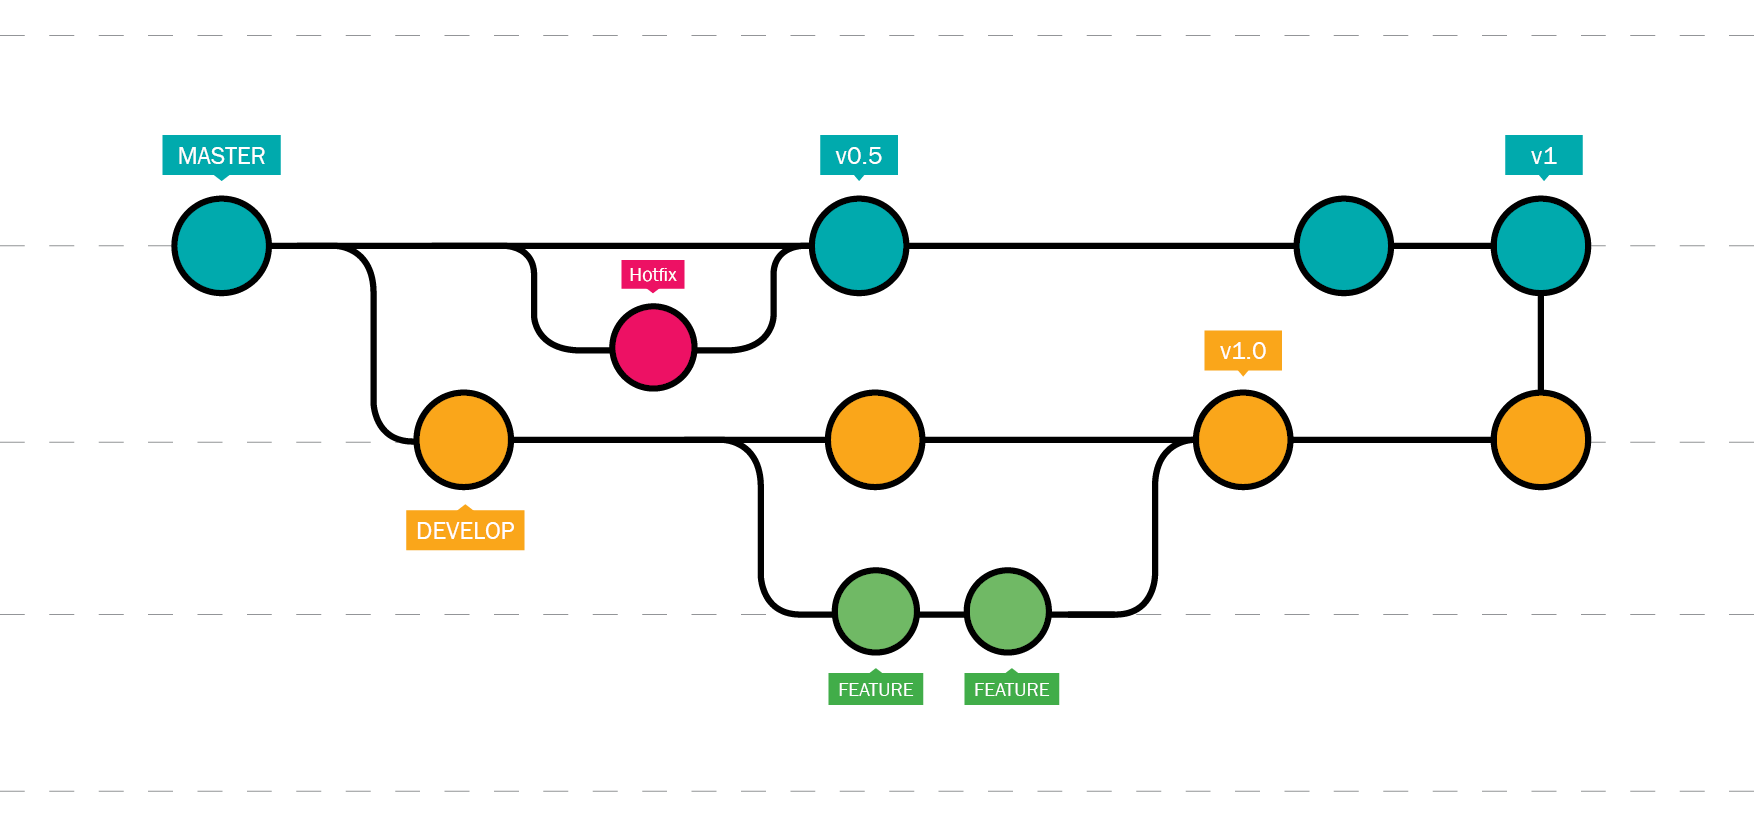
\includegraphics[keepaspectratio]{img/05_Ramas/ejemplo-rama.png}}

Podemos ver a las ramas como lineas donde la rama \texttt{main/master} es la linea central, mientras que las ramas que se desprenden de esta avanzan de forma paralela a la principal, lo que permite tomar caminos distintos sin alterar la rama principal.

\textbf{La Rama \texttt{main}}

Es como la \textbf{sagrada línea del tiempo} del multiverso. Es la versión principal y estable de la historia, donde los eventos más importantes suceden.

\begin{itemize}
\tightlist
\item
  \textbf{Ejemplo:}
\end{itemize}

En el MCU, la sagrada línea del tiempo incluye eventos clave como la creación de los Vengadores, la batalla contra Thanos, y el sacrificio de Tony Stark.

Crear una rama en Git significa generar una línea paralela de desarrollo en el repositorio. Esto te permite trabajar en cambios o características nuevas de forma aislada, sin afectar la rama principal (main o master)

\textbf{Crear una Rama}

Es como generar una \textbf{realidad alternativa} dentro del multiverso. Esta nueva línea puede desarrollarse de manera independiente sin afectar la línea principal hasta que decidas unirlas.

\begin{itemize}
\tightlist
\item
  \textbf{Ejemplo:}
\end{itemize}

Cuando Loki toma el Tesseract en \emph{Avengers: Endgame}, crea una nueva línea temporal. Esa nueva línea no afecta la sagrada hasta que interactúe directamente con ella.

Moverse entre ramas en Git significa cambiar el contexto de trabajo para apuntar a una rama específica. Esto actualiza el estado del directorio de trabajo al contenido de la rama seleccionada, incluyendo los archivos y la referencia de commits.

\textbf{Moverse Entre Ramas}
Es como \textbf{cambiar de una realidad a otra}. Puedes viajar entre estas realidades alternativas para trabajar en diferentes historias sin perder el contexto de cada una.

\begin{itemize}
\tightlist
\item
  \textbf{Ejemplo:}
\end{itemize}

Doctor Strange usando el Darkhold para explorar diferentes universos en \emph{Doctor Strange in the Multiverse of Madness}. Cambia entre realidades para lograr un objetivo específico.

Como parte del uso de las ramas, contamos con la posibiliad de tomar los cambios realizados en una rama y llevarlos a la rama principal, por ejemplo en caso de haber terminado la implmentación de una nueva característica, podemos llevar todo ese trabajo a la rama \texttt{main/master} para incluir dicha implementación, esto se a través del \texttt{merge}.

\textbf{Merge}: Es el proceso de combinar cambios de diferentes ramas en una sola rama.

\pandocbounded{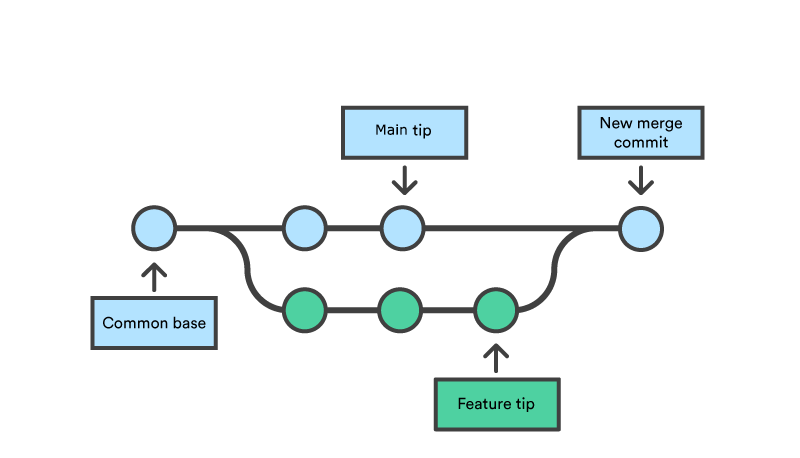
\includegraphics[keepaspectratio]{img/05_Ramas/ejemplo-merge.png}}

\textbf{Unir Ramas (Merge)}
Es como \textbf{fusionar realidades alternativas con la sagrada línea del tiempo}. Al hacerlo, introduces los cambios (o eventos) de la línea alternativa en la principal.

\begin{itemize}
\tightlist
\item
  \textbf{Ejemplo:}
\end{itemize}

En \emph{Spider-Man: No Way Home}, las líneas temporales de los otros Spider-Man (Tobey Maguire y Andrew Garfield) se unen con la línea de Tom Holland para enfrentar un desafío común.

Este proceso se puede realizar de distintas maneras:

\begin{itemize}
\tightlist
\item
  \textbf{Fast-forward}: Un fast-forward en Git es una fusión en la que la rama de destino avanza directamente al nuevo commit sin crear un commit de fusión.
\end{itemize}

\pandocbounded{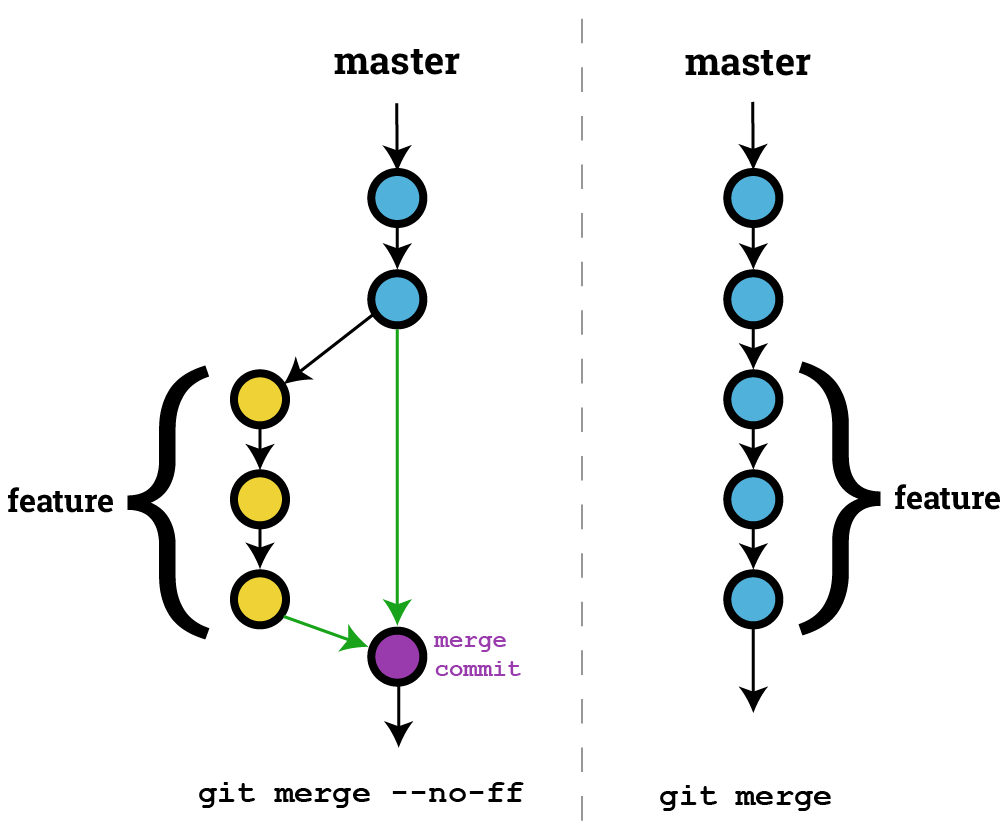
\includegraphics[keepaspectratio]{img/05_Ramas/ejemplo-fast-forward.png}}

\textbf{Fast-Forward}

El fast-forward ocurre cuando una rama no tiene cambios adicionales y se puede mover directamente hacia la rama principal. Es como \textbf{seguir la línea sagrada sin crear ramas alternas complicadas}.

\begin{itemize}
\tightlist
\item
  \textbf{Ejemplo:}
\end{itemize}

En \emph{Loki}, si una variante sigue exactamente los pasos de la línea sagrada, no necesita intervención de la TVA para mantenerse alineada.

\begin{itemize}
\tightlist
\item
  \textbf{Unión automática (Automatic merge)}: Una unión automática en Git es cuando Git fusiona automáticamente cambios de diferentes ramas sin conflictos manuales.
\end{itemize}

\pandocbounded{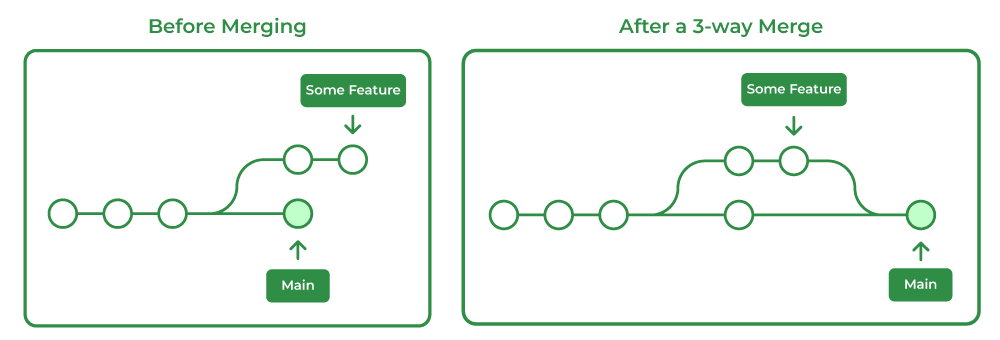
\includegraphics[keepaspectratio]{img/05_Ramas/ejemplo-union-automatica.png}}

\textbf{Automatic Merge}

Un merge automático ocurre cuando las diferencias entre ramas se combinan sin conflicto.

\begin{itemize}
\tightlist
\item
  \textbf{Ejemplo:}
\end{itemize}

En \emph{Infinity War}, los Guardianes de la Galaxia y los Vengadores unen fuerzas sin problemas iniciales para detener a Thanos.

\begin{itemize}
\tightlist
\item
  \textbf{Unión manual (Manual merge)}: Una unión manual en Git ocurre cuando se requieren resoluciones de conflictos por parte del usuario durante el proceso de fusión entre ramas.
\end{itemize}

\pandocbounded{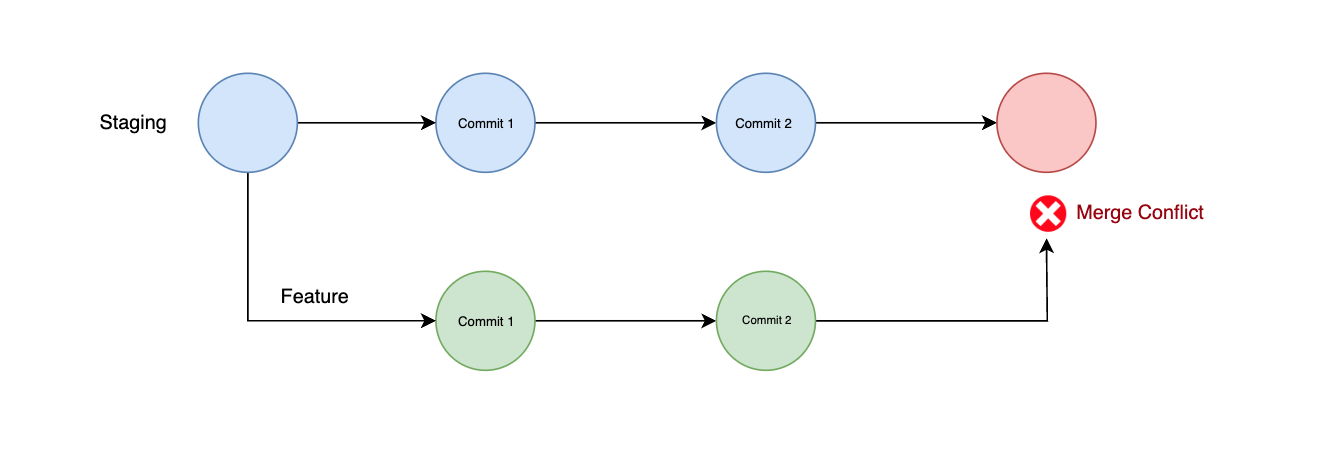
\includegraphics[keepaspectratio]{img/05_Ramas/ejemplo-union-manual.png}}

\textbf{Manual Merge}

Es necesario cuando hay conflictos que deben resolverse antes de completar la fusión.

\begin{itemize}
\tightlist
\item
  \textbf{Ejemplo:}
\end{itemize}

En \emph{Civil War}, los héroes intentan trabajar juntos, pero las diferencias entre Tony Stark y Steve Rogers provocan un conflicto que necesita solución antes de seguir adelante.

Es evidente que las el uso de las ramas es muy útil en el desarrollo de cualquier proyecto, pues nos permite hacer nuevas implementaciones y/o cambios en el código sin afectar la rama principal del repositorio.

\section{Merge: Fast-forward}\label{merge-fast-forward}

Seguiremos trabajando con el material \texttt{material-marvel}asi que nos colocaremos desde la terminal en la ubicacion del material y seguiremos las siguientes instrucciones:

\begin{enumerate}
\def\labelenumi{\arabic{enumi}.}
\tightlist
\item
  Para listar las ramas que tenemos en el repositorio emplearemos:
\end{enumerate}

\begin{Shaded}
\begin{Highlighting}[]
\FunctionTok{git}\NormalTok{ branch}
\end{Highlighting}
\end{Shaded}

\begin{Shaded}
\begin{Highlighting}[]
\ExtensionTok{*}\NormalTok{ main}
\end{Highlighting}
\end{Shaded}

\begin{enumerate}
\def\labelenumi{\arabic{enumi}.}
\setcounter{enumi}{1}
\tightlist
\item
  Supongamos ahora que hay héroes de Tierra-99999 que se quieren unir a nuestra agrupación principal de héroes por lo que haremos una nueva rama del registro para incorporarlos mientras se evaluan sus aptitudes para integrarse al equipo:
\end{enumerate}

\begin{Shaded}
\begin{Highlighting}[]
\FunctionTok{git}\NormalTok{ branch tierra{-}99999}
\end{Highlighting}
\end{Shaded}

Si volvemos a listar las ramas, encontraremos esta nueva rama que acabamos de crear:

\begin{Shaded}
\begin{Highlighting}[]
\FunctionTok{git}\NormalTok{ branch}
\end{Highlighting}
\end{Shaded}

\begin{Shaded}
\begin{Highlighting}[]
\ExtensionTok{*}\NormalTok{ main}
  \ExtensionTok{tierra{-}99999}
\end{Highlighting}
\end{Shaded}

Aquí podemos notar que Git nos indica la rama en la que nos encontramos a través de un asterisco \texttt{*} que precede al nombre de la rama sobre la que nos ubicamos, en este caso la rama \texttt{main}

Como el registo es para los héroes de tierra-99999, vamos a cambiar a la rama que acabamos de crear:

\begin{Shaded}
\begin{Highlighting}[]
\FunctionTok{git}\NormalTok{ checkout tierra{-}99999}
\end{Highlighting}
\end{Shaded}

\begin{Shaded}
\begin{Highlighting}[]
\ExtensionTok{Cambiado}\NormalTok{ a rama }\StringTok{\textquotesingle{}tierra{-}99999\textquotesingle{}}
\end{Highlighting}
\end{Shaded}

Ahora, si listamos los cambios de nuestro repositorio, notaremos algo interesante:

\begin{Shaded}
\begin{Highlighting}[]
\FunctionTok{git}\NormalTok{ lg}
\end{Highlighting}
\end{Shaded}

\begin{Shaded}
\begin{Highlighting}[]
\ExtensionTok{*}\NormalTok{ c20b80d }\AttributeTok{{-}} \ErrorTok{(}\ExtensionTok{hace}\NormalTok{ 4 minutos}\KeywordTok{)} \ExtensionTok{.gitignore}\NormalTok{ actualizado }\ErrorTok{(}\ExtensionTok{extension}\NormalTok{ .log}\KeywordTok{)} \ExtensionTok{{-}}\NormalTok{ [Nombre de usuario] }\ErrorTok{(}\ExtensionTok{HEAD} \AttributeTok{{-}}\OperatorTok{\textgreater{}}\NormalTok{ tierra{-}99999, main}\KeywordTok{)}
\ExtensionTok{*}\NormalTok{ 2ed8cf4 }\AttributeTok{{-}} \ErrorTok{(}\ExtensionTok{hace}\NormalTok{ 5 minutos}\KeywordTok{)} \ExtensionTok{.gitignore}\NormalTok{ agregado }\AttributeTok{{-}}\NormalTok{ [Nombre de usuario]}
\ExtensionTok{*}\NormalTok{ c9ffd15 }\AttributeTok{{-}} \ErrorTok{(}\ExtensionTok{hace}\NormalTok{ 10 minutos}\KeywordTok{)} \ExtensionTok{sin}\NormalTok{ saignaciones para Spider{-}Man }\AttributeTok{{-}}\NormalTok{ [Nombre de usuario]}
\ExtensionTok{*}\NormalTok{ e31eae6 }\AttributeTok{{-}} \ErrorTok{(}\ExtensionTok{hace}\NormalTok{ 14 minutos}\KeywordTok{)} \ExtensionTok{misiones}\NormalTok{ de Spider{-}Man completadas }\AttributeTok{{-}}\NormalTok{ [Nombre de usuario]}
\ExtensionTok{*}\NormalTok{ 0059540 }\AttributeTok{{-}} \ErrorTok{(}\ExtensionTok{hace}\NormalTok{ 15 minutos}\KeywordTok{)} \ExtensionTok{contactos.md}\NormalTok{ eliminado }\AttributeTok{{-}}\NormalTok{ [Nombre de usuario]}
\ExtensionTok{*}\NormalTok{ 2d05f6e }\AttributeTok{{-}} \ErrorTok{(}\ExtensionTok{hace}\NormalTok{ 18 minutos}\KeywordTok{)} \ExtensionTok{contactos.md}\NormalTok{ renombrado }\AttributeTok{{-}}\NormalTok{ [Nombre de usuario]}
\ExtensionTok{*}\NormalTok{ 1c7fe32 }\AttributeTok{{-}} \ErrorTok{(}\ExtensionTok{hace}\NormalTok{ 19 minutos}\KeywordTok{)} \ExtensionTok{contactos}\NormalTok{ de emergencia agregados }\AttributeTok{{-}}\NormalTok{ [Nombre de usuario]}
\ExtensionTok{*}\NormalTok{ 8727c32 }\AttributeTok{{-}} \ErrorTok{(}\ExtensionTok{hace}\NormalTok{ 26 minutos}\KeywordTok{)} \ExtensionTok{se}\NormalTok{ unen Doctor Strange y Daredevil }\AttributeTok{{-}}\NormalTok{ [Nombre de usuario]}
\ExtensionTok{*}\NormalTok{ a2427e8 }\AttributeTok{{-}} \ErrorTok{(}\ExtensionTok{hace}\NormalTok{ 43 minutos}\KeywordTok{)} \ExtensionTok{misiones/}\NormalTok{ agregado }\AttributeTok{{-}}\OperatorTok{\textgreater{}}\NormalTok{ misiones de los heroes: iron man, thor, hulk, black widow y spider man. }\AttributeTok{{-}}\NormalTok{ [Nombre de usuario]}
\ExtensionTok{*}\NormalTok{ 43b3a69 }\AttributeTok{{-}} \ErrorTok{(}\ExtensionTok{hace}\NormalTok{ 44 minutos}\KeywordTok{)} \ExtensionTok{debilidades.md}\NormalTok{ agregado }\AttributeTok{{-}}\NormalTok{ [Nombre de usuario]}
\ExtensionTok{*}\NormalTok{ c691147 }\AttributeTok{{-}} \ErrorTok{(}\ExtensionTok{hace}\NormalTok{ 44 minutos}\KeywordTok{)} \ExtensionTok{origenes.md}\NormalTok{ agregado }\AttributeTok{{-}}\NormalTok{ [Nombre de usuario]}
\ExtensionTok{*}\NormalTok{ ec89c02 }\AttributeTok{{-}} \ErrorTok{(}\ExtensionTok{hace}\NormalTok{ 45 minutos}\KeywordTok{)} \ExtensionTok{descripciones.md}\NormalTok{ agregado }\AttributeTok{{-}}\NormalTok{ [Nombre de usuario]}
\ExtensionTok{*}\NormalTok{ ac02fe0 }\AttributeTok{{-}} \ErrorTok{(}\ExtensionTok{hace}\NormalTok{ 45 minutos}\KeywordTok{)} \ExtensionTok{README.md}\NormalTok{ agregado }\AttributeTok{{-}}\NormalTok{ [Nombre de usuario]\%}
\end{Highlighting}
\end{Shaded}

Además de aparecer los nuevos commits que realizamos, podemos notar que al final de la primer línea, tenemos \texttt{(HEAD\ -\textgreater{}\ tierra-99999,\ main)}, lo que nos indica que el último commit registrado por las ramas \texttt{main} y \texttt{tierra-99999} es el mismo, es decir, ambas estan en el mismo punto del repositorio, tambien podemos notar que no ha cambiado nada en los archivos o directorios.

\begin{enumerate}
\def\labelenumi{\arabic{enumi}.}
\setcounter{enumi}{2}
\tightlist
\item
  Procediendo a hacer modificaciones en el repositorio.
\end{enumerate}

Vamos a crear el registro de los siguientes dos heroes: \texttt{Captain\ Marvel} y \texttt{Doctor\ Doom}, por lo que modificaremos los archivos \texttt{Readme.md}, \texttt{descripciones.md}, \texttt{origenes.md}, \texttt{debilidades.md} y les asignaremos misiones a cada uno.

Para el archivo \texttt{descripciones.md} agregamos:

\begin{Shaded}
\begin{Highlighting}[]

\CommentTok{\#\# Captain Marvel}

\ExtensionTok{{-}} \PreprocessorTok{**}\NormalTok{Nombre real:}\PreprocessorTok{**}\NormalTok{ Carol Danvers}
\ExtensionTok{{-}} \PreprocessorTok{**}\NormalTok{Descripción:}\PreprocessorTok{**}\NormalTok{ Proviene de una dimensión alterna donde los Kree y los Skrulls se aliaron para derrotar a los humanos. Su poder proviene de una combinación de ADN humano y Kree.}

\CommentTok{\#\# Doctor Doom}

\ExtensionTok{{-}} \PreprocessorTok{**}\NormalTok{Nombre real:}\PreprocessorTok{**}\NormalTok{ Victor Von Doom}
\ExtensionTok{{-}} \PreprocessorTok{**}\NormalTok{Descripción:}\PreprocessorTok{**}\NormalTok{ Un genio y hechicero de la dimensión alterna que combina ciencia avanzada con magia. A pesar de su ego y su búsqueda de poder, también lucha por la paz a su manera.}
\end{Highlighting}
\end{Shaded}

Al archivo \texttt{origenes.md} se le agrega:

\begin{Shaded}
\begin{Highlighting}[]

\CommentTok{\#\# Captain Marvel}

\ExtensionTok{{-}}\NormalTok{ Un accidente relacionado con una tecnología alienígena la expuso a la energía de un artefacto Kree, lo que alteró su biología.}

\CommentTok{\#\# Doctor Doom}

\ExtensionTok{{-}}\NormalTok{ Después de perder a su madre en un ritual mágico que salió mal, tomó el control de su nación para asegurar la paz bajo su dominio.}
\end{Highlighting}
\end{Shaded}

Para el archivo \texttt{debilidades.md} añadimos:

\begin{Shaded}
\begin{Highlighting}[]

\CommentTok{\#\# Captain Marvel}

\ExtensionTok{{-}}\NormalTok{ Vulnerabilidad a la magia }
\ExtensionTok{{-}}\NormalTok{ Su conexión con el poder de la Fuerza Kree puede ser inestable.}

\CommentTok{\#\# Doctor Doom}

\ExtensionTok{{-}}\NormalTok{ Vulnerable a la magia y al control mental.}
\ExtensionTok{{-}}\NormalTok{ Su obsesión con el control absoluto lo hace susceptible a tomar decisiones que pueden llevar a su caída.}
\end{Highlighting}
\end{Shaded}

Para las misiones, generamos un nuevo registro para cada uno.

Las misiones agregadas a \texttt{misiones/captain\_marvel\_t-99999.md}:

\begin{Shaded}
\begin{Highlighting}[]
\CommentTok{\# Misiones de Captain Marvel}

\ExtensionTok{1.} \PreprocessorTok{**}\NormalTok{Defender la estación espacial de una invasión Skrull}\PreprocessorTok{**}
   
   \ExtensionTok{{-}}\NormalTok{ Descripción: Detener el ataque de los Skrulls y proteger la estación espacial en el borde de la galaxia.}
   \ExtensionTok{{-}}\NormalTok{ Prioridad: Alta}
   \ExtensionTok{{-}}\NormalTok{ Fecha límite: 2025{-}02{-}01}

\ExtensionTok{2.} \PreprocessorTok{**}\NormalTok{Investigar una anomalía en el espacio{-}tiempo}\PreprocessorTok{**}
   
   \ExtensionTok{{-}}\NormalTok{ Descripción: Analizar una distorsión en el espacio{-}tiempo que está afectando las rutas de navegación interdimensional.}
   \ExtensionTok{{-}}\NormalTok{ Prioridad: Media}
   \ExtensionTok{{-}}\NormalTok{ Fecha límite: 2025{-}03{-}01}

\ExtensionTok{3.} \PreprocessorTok{**}\NormalTok{Colaborar con otras dimensiones para evitar el colapso de los multiversos}\PreprocessorTok{**}
   
   \ExtensionTok{{-}}\NormalTok{ Descripción: Unirse a héroes de otras realidades para prevenir una crisis que podría destruir las fronteras entre los universos.}
   \ExtensionTok{{-}}\NormalTok{ Prioridad: Alta}
   \ExtensionTok{{-}}\NormalTok{ Fecha límite: 2025{-}03{-}15}
\end{Highlighting}
\end{Shaded}

Las misiones agregadas a \texttt{misiones/doctor\_doom\_t-99999.md}:

\begin{Shaded}
\begin{Highlighting}[]
\CommentTok{\# Misiones de Doctor Doom}

\ExtensionTok{1.} \PreprocessorTok{**}\NormalTok{Conquistar una ciudad en una dimensión paralela}\PreprocessorTok{**}
   
   \ExtensionTok{{-}}\NormalTok{ Descripción: Invadir y tomar el control de una ciudad en una dimensión alternativa para expandir su imperio.}
   \ExtensionTok{{-}}\NormalTok{ Prioridad: Alta}
   \ExtensionTok{{-}}\NormalTok{ Fecha límite: 2025{-}02{-}10}

\ExtensionTok{2.} \PreprocessorTok{**}\NormalTok{Investigar una antigua reliquia mágica}\PreprocessorTok{**}
   
   \ExtensionTok{{-}}\NormalTok{ Descripción: Desentrañar los secretos de un artefacto místico para incrementar sus habilidades mágicas y científicas.}
   \ExtensionTok{{-}}\NormalTok{ Prioridad: Alta}
   \ExtensionTok{{-}}\NormalTok{ Fecha límite: 2025{-}02{-}20}

\ExtensionTok{3.} \PreprocessorTok{**}\NormalTok{Frenar un cataclismo dimensional causado por un enemigo desconocido}\PreprocessorTok{**}
   
   \ExtensionTok{{-}}\NormalTok{ Descripción: Detener el colapso de múltiples realidades que amenaza con destruir el multiverso.}
   \ExtensionTok{{-}}\NormalTok{ Prioridad: Alta}
   \ExtensionTok{{-}}\NormalTok{ Fecha límite: 2025{-}03{-}01}
\end{Highlighting}
\end{Shaded}

Verificando el estado del repositorio:

\begin{Shaded}
\begin{Highlighting}[]
\FunctionTok{git}\NormalTok{ s}
\end{Highlighting}
\end{Shaded}

\begin{Shaded}
\begin{Highlighting}[]
\CommentTok{\#\# tierra{-}99999}
 \ExtensionTok{M}\NormalTok{ debilidades.md}
 \ExtensionTok{M}\NormalTok{ descripciones.md}
 \ExtensionTok{M}\NormalTok{ origenes.md}
\ExtensionTok{??}\NormalTok{ misiones/captain\_marvel\_t{-}99999.md}
\ExtensionTok{??}\NormalTok{ misiones/doctor\_doom\_t{-}99999.md}
\end{Highlighting}
\end{Shaded}

\begin{enumerate}
\def\labelenumi{\arabic{enumi}.}
\setcounter{enumi}{3}
\tightlist
\item
  Agregamos todo al Stage y hacemos un commit
\end{enumerate}

\begin{Shaded}
\begin{Highlighting}[]
\FunctionTok{git}\NormalTok{ add .}
\end{Highlighting}
\end{Shaded}

\begin{Shaded}
\begin{Highlighting}[]
\FunctionTok{git}\NormalTok{ commit }\AttributeTok{{-}m} \StringTok{"se unen Captain marvel y Doctor Doom de Tierra{-}99999"}
\end{Highlighting}
\end{Shaded}

\begin{Shaded}
\begin{Highlighting}[]
\ExtensionTok{[tierra{-}99999}\NormalTok{ 6976c5a] se unen Captain marvel y Doctor Doom de Tierra{-}99999}
 \ExtensionTok{5}\NormalTok{ files changed, 66 insertions}\ErrorTok{(}\ExtensionTok{+}\KeywordTok{)}
 \ExtensionTok{create}\NormalTok{ mode 100644 misiones/captain\_marvel\_t{-}99999.md}
 \ExtensionTok{create}\NormalTok{ mode 100644 misiones/doctor\_doom\_t{-}99999.md}
\end{Highlighting}
\end{Shaded}

\begin{enumerate}
\def\labelenumi{\arabic{enumi}.}
\setcounter{enumi}{4}
\tightlist
\item
  Listamos los registros:
\end{enumerate}

\begin{Shaded}
\begin{Highlighting}[]
\FunctionTok{git}\NormalTok{ lg}
\end{Highlighting}
\end{Shaded}

\begin{Shaded}
\begin{Highlighting}[]
\ExtensionTok{*}\NormalTok{ 6976c5a }\AttributeTok{{-}} \ErrorTok{(}\ExtensionTok{hace}\NormalTok{ 26 segundos}\KeywordTok{)} \ExtensionTok{se}\NormalTok{ unen Captain marvel y Doctor Doom de Tierra{-}99999 }\AttributeTok{{-}}\NormalTok{ [Nombre de usuario] }\ErrorTok{(}\ExtensionTok{HEAD} \AttributeTok{{-}}\OperatorTok{\textgreater{}}\NormalTok{ tierra{-}99999}\KeywordTok{)}
\ExtensionTok{*}\NormalTok{ c20b80d }\AttributeTok{{-}} \ErrorTok{(}\ExtensionTok{hace}\NormalTok{ 8 minutos}\KeywordTok{)} \ExtensionTok{.gitignore}\NormalTok{ actualizado }\ErrorTok{(}\ExtensionTok{extension}\NormalTok{ .log}\KeywordTok{)} \ExtensionTok{{-}}\NormalTok{ [Nombre de usuario] }\ErrorTok{(}\ExtensionTok{main}\KeywordTok{)}
\ExtensionTok{*}\NormalTok{ 2ed8cf4 }\AttributeTok{{-}} \ErrorTok{(}\ExtensionTok{hace}\NormalTok{ 10 minutos}\KeywordTok{)} \ExtensionTok{.gitignore}\NormalTok{ agregado }\AttributeTok{{-}}\NormalTok{ [Nombre de usuario]}
\ExtensionTok{*}\NormalTok{ c9ffd15 }\AttributeTok{{-}} \ErrorTok{(}\ExtensionTok{hace}\NormalTok{ 14 minutos}\KeywordTok{)} \ExtensionTok{sin}\NormalTok{ saignaciones para Spider{-}Man }\AttributeTok{{-}}\NormalTok{ [Nombre de usuario]}
\ExtensionTok{*}\NormalTok{ e31eae6 }\AttributeTok{{-}} \ErrorTok{(}\ExtensionTok{hace}\NormalTok{ 19 minutos}\KeywordTok{)} \ExtensionTok{misiones}\NormalTok{ de Spider{-}Man completadas }\AttributeTok{{-}}\NormalTok{ [Nombre de usuario]}
\ExtensionTok{*}\NormalTok{ 0059540 }\AttributeTok{{-}} \ErrorTok{(}\ExtensionTok{hace}\NormalTok{ 19 minutos}\KeywordTok{)} \ExtensionTok{contactos.md}\NormalTok{ eliminado }\AttributeTok{{-}}\NormalTok{ [Nombre de usuario]}
\ExtensionTok{*}\NormalTok{ 2d05f6e }\AttributeTok{{-}} \ErrorTok{(}\ExtensionTok{hace}\NormalTok{ 22 minutos}\KeywordTok{)} \ExtensionTok{contactos.md}\NormalTok{ renombrado }\AttributeTok{{-}}\NormalTok{ [Nombre de usuario]}
\ExtensionTok{*}\NormalTok{ 1c7fe32 }\AttributeTok{{-}} \ErrorTok{(}\ExtensionTok{hace}\NormalTok{ 23 minutos}\KeywordTok{)} \ExtensionTok{contactos}\NormalTok{ de emergencia agregados }\AttributeTok{{-}}\NormalTok{ [Nombre de usuario]}
\ExtensionTok{*}\NormalTok{ 8727c32 }\AttributeTok{{-}} \ErrorTok{(}\ExtensionTok{hace}\NormalTok{ 30 minutos}\KeywordTok{)} \ExtensionTok{se}\NormalTok{ unen Doctor Strange y Daredevil }\AttributeTok{{-}}\NormalTok{ [Nombre de usuario]}
\ExtensionTok{*}\NormalTok{ a2427e8 }\AttributeTok{{-}} \ErrorTok{(}\ExtensionTok{hace}\NormalTok{ 48 minutos}\KeywordTok{)} \ExtensionTok{misiones/}\NormalTok{ agregado }\AttributeTok{{-}}\OperatorTok{\textgreater{}}\NormalTok{ misiones de los heroes: iron man, thor, hulk, black widow y spider man. }\AttributeTok{{-}}\NormalTok{ [Nombre de usuario]}
\ExtensionTok{*}\NormalTok{ 43b3a69 }\AttributeTok{{-}} \ErrorTok{(}\ExtensionTok{hace}\NormalTok{ 48 minutos}\KeywordTok{)} \ExtensionTok{debilidades.md}\NormalTok{ agregado }\AttributeTok{{-}}\NormalTok{ [Nombre de usuario]}
\ExtensionTok{*}\NormalTok{ c691147 }\AttributeTok{{-}} \ErrorTok{(}\ExtensionTok{hace}\NormalTok{ 49 minutos}\KeywordTok{)} \ExtensionTok{origenes.md}\NormalTok{ agregado }\AttributeTok{{-}}\NormalTok{ [Nombre de usuario]}
\ExtensionTok{*}\NormalTok{ ec89c02 }\AttributeTok{{-}} \ErrorTok{(}\ExtensionTok{hace}\NormalTok{ 49 minutos}\KeywordTok{)} \ExtensionTok{descripciones.md}\NormalTok{ agregado }\AttributeTok{{-}}\NormalTok{ [Nombre de usuario]}
\ExtensionTok{*}\NormalTok{ ac02fe0 }\AttributeTok{{-}} \ErrorTok{(}\ExtensionTok{hace}\NormalTok{ 50 minutos}\KeywordTok{)} \ExtensionTok{README.md}\NormalTok{ agregado }\AttributeTok{{-}}\NormalTok{ [Nombre de usuario]\%        }
\end{Highlighting}
\end{Shaded}

Podemos notar que la rama \texttt{main} se queda un commit por debajo de \texttt{tierra-99999}, que ahora es el \texttt{HEAD}, esto porque los cambios que registramos solo afectan a la rama actual, \texttt{tierra-99999}.

\begin{enumerate}
\def\labelenumi{\arabic{enumi}.}
\setcounter{enumi}{5}
\tightlist
\item
  Al poco tiempo se une también \texttt{Scarlet\ Which}, por lo que hacemos su registro.
\end{enumerate}

Para el archivo \texttt{descripciones.md} agregamos:

\begin{Shaded}
\begin{Highlighting}[]

\CommentTok{\#\# Scarlet Witch}

\ExtensionTok{{-}} \PreprocessorTok{**}\NormalTok{Nombre real:}\PreprocessorTok{**}\NormalTok{ Wanda Maximoff}
\ExtensionTok{{-}} \PreprocessorTok{**}\NormalTok{Descripción:}\PreprocessorTok{**}\NormalTok{ Una poderosa hechicera que perfeccionó su control del caos y del multiverso.}
\end{Highlighting}
\end{Shaded}

Al archivo \texttt{origenes.md} se le agrega:

\begin{Shaded}
\begin{Highlighting}[]

\CommentTok{\#\# Scarlet Witch}

\ExtensionTok{{-}}\NormalTok{ Descubrió el Grimorio Oscuro a una edad temprana, lo que la llevó a comprender y controlar la magia del caos de manera más efectiva.}
\end{Highlighting}
\end{Shaded}

Para el archivo \texttt{debilidades.md} añadimos:

\begin{Shaded}
\begin{Highlighting}[]

\CommentTok{\#\# Scarlet Witch}

\ExtensionTok{{-}}\NormalTok{ Vulnerable a ataques psíquicos de alta intensidad y al desgaste emocionalmente}
\ExtensionTok{{-}}\NormalTok{ El uso prolongado del Grimorio Oscuro puede corroer su mente.}
\end{Highlighting}
\end{Shaded}

Para las misiones, generamos un nuevo registro para cada uno.

Las misiones agregadas a \texttt{misiones/scarlet\_witch\_t-99999.md}:

\begin{Shaded}
\begin{Highlighting}[]
\CommentTok{\# Misiones de Scarlet Witch}

\ExtensionTok{1.} \PreprocessorTok{**}\NormalTok{Reparar los portales dimensionales dañados}\PreprocessorTok{**}

   \ExtensionTok{{-}}\NormalTok{ Descripción: Utilizar su magia para estabilizar los portales que conectan Tierra{-}99999 con otras dimensiones.}
   \ExtensionTok{{-}}\NormalTok{ Prioridad: Alta}
   \ExtensionTok{{-}}\NormalTok{ Fecha límite: 2025{-}02{-}15}

\ExtensionTok{2.} \PreprocessorTok{**}\NormalTok{Neutralizar una convergencia mágica inestable}\PreprocessorTok{**}

   \ExtensionTok{{-}}\NormalTok{ Descripción: Identificar y detener un evento en el que múltiples líneas temporales intentan fusionarse.}
   \ExtensionTok{{-}}\NormalTok{ Prioridad: Alta}
   \ExtensionTok{{-}}\NormalTok{ Fecha límite: 2025{-}03{-}05}

\ExtensionTok{3.} \PreprocessorTok{**}\NormalTok{Recuperar el Grimorio Perdido}\PreprocessorTok{**}

   \ExtensionTok{{-}}\NormalTok{ Descripción: Localizar un grimorio antiguo que contiene conocimientos esenciales para prevenir un apocalipsis multiversal.}
   \ExtensionTok{{-}}\NormalTok{ Prioridad: Media}
   \ExtensionTok{{-}}\NormalTok{ Fecha límite: 2025{-}03{-}20}
\end{Highlighting}
\end{Shaded}

Para este punto los héroes de \texttt{tierra-99999} muestran ser buenos elementos por lo que se les agrega al registro principal, en el archivo \texttt{README.md}, al que se le añade:

\begin{Shaded}
\begin{Highlighting}[]
  \ExtensionTok{{-}}\NormalTok{ [captain marvel }\ErrorTok{(}\ExtensionTok{T{-}99999}\KeywordTok{)}\ExtensionTok{]}\ErrorTok{(}\ExtensionTok{/misiones/captain\_marvel\_t{-}99999.md}\KeywordTok{)}
  \ExtensionTok{{-}}\NormalTok{ [doctor doom }\ErrorTok{(}\ExtensionTok{T{-}99999}\KeywordTok{)}\ExtensionTok{]}\ErrorTok{(}\ExtensionTok{/misiones/doctor\_doom\_t{-}99999.md}\KeywordTok{)}
  \ExtensionTok{{-}}\NormalTok{ [scarlet witch }\ErrorTok{(}\ExtensionTok{T{-}99999}\KeywordTok{)}\ExtensionTok{]}\ErrorTok{(}\ExtensionTok{/misiones/scarlet\_witch\_t{-}99999.md}\KeywordTok{)}
\end{Highlighting}
\end{Shaded}

Verificando el estado del repositorio:

\begin{Shaded}
\begin{Highlighting}[]
\FunctionTok{git}\NormalTok{ s}
\end{Highlighting}
\end{Shaded}

\begin{Shaded}
\begin{Highlighting}[]
\CommentTok{\#\# tierra{-}99999}
 \ExtensionTok{M}\NormalTok{ README.md}
 \ExtensionTok{M}\NormalTok{ debilidades.md}
 \ExtensionTok{M}\NormalTok{ descripciones.md}
 \ExtensionTok{M}\NormalTok{ origenes.md}
\ExtensionTok{??}\NormalTok{ misiones/scarlet\_witch\_t{-}99999.md}
\end{Highlighting}
\end{Shaded}

\begin{enumerate}
\def\labelenumi{\arabic{enumi}.}
\setcounter{enumi}{6}
\tightlist
\item
  Agregamos al Stage y hacemos un commit
\end{enumerate}

\begin{Shaded}
\begin{Highlighting}[]
\FunctionTok{git}\NormalTok{ add .}
\end{Highlighting}
\end{Shaded}

\begin{Shaded}
\begin{Highlighting}[]
\FunctionTok{git}\NormalTok{ commit }\AttributeTok{{-}m} \StringTok{"se une Scarlet Witch de Tierra{-}99999; se termina el registro de T{-}99999"}
\end{Highlighting}
\end{Shaded}

\begin{Shaded}
\begin{Highlighting}[]
\ExtensionTok{[tierra{-}99999}\NormalTok{ f5907d1] se une Scarlet Witch de Tierra{-}99999}\KeywordTok{;} \ExtensionTok{se}\NormalTok{ termina el registro de T{-}99999}
 \ExtensionTok{5}\NormalTok{ files changed, 36 insertions}\ErrorTok{(}\ExtensionTok{+}\KeywordTok{)}
 \ExtensionTok{create}\NormalTok{ mode 100644 misiones/scarlet\_witch\_t{-}99999.md}
\end{Highlighting}
\end{Shaded}

\begin{enumerate}
\def\labelenumi{\arabic{enumi}.}
\setcounter{enumi}{7}
\tightlist
\item
  Listamos los registros:
\end{enumerate}

\begin{Shaded}
\begin{Highlighting}[]
\FunctionTok{git}\NormalTok{ lg}
\end{Highlighting}
\end{Shaded}

\begin{Shaded}
\begin{Highlighting}[]
\ExtensionTok{*}\NormalTok{ f5907d1 }\AttributeTok{{-}} \ErrorTok{(}\ExtensionTok{hace}\NormalTok{ 18 segundos}\KeywordTok{)} \ExtensionTok{se}\NormalTok{ une Scarlet Witch de Tierra{-}99999}\KeywordTok{;} \ExtensionTok{se}\NormalTok{ termina el registro de T{-}99999 }\AttributeTok{{-}}\NormalTok{ [Nombre de usuario] }\ErrorTok{(}\ExtensionTok{HEAD} \AttributeTok{{-}}\OperatorTok{\textgreater{}}\NormalTok{ tierra{-}99999}\KeywordTok{)}
\ExtensionTok{*}\NormalTok{ 6976c5a }\AttributeTok{{-}} \ErrorTok{(}\ExtensionTok{hace}\NormalTok{ 5 minutos}\KeywordTok{)} \ExtensionTok{se}\NormalTok{ unen Captain marvel y Doctor Doom de Tierra{-}99999 }\AttributeTok{{-}}\NormalTok{ [Nombre de usuario]}
\ExtensionTok{*}\NormalTok{ c20b80d }\AttributeTok{{-}} \ErrorTok{(}\ExtensionTok{hace}\NormalTok{ 12 minutos}\KeywordTok{)} \ExtensionTok{.gitignore}\NormalTok{ actualizado }\ErrorTok{(}\ExtensionTok{extension}\NormalTok{ .log}\KeywordTok{)} \ExtensionTok{{-}}\NormalTok{ [Nombre de usuario] }\ErrorTok{(}\ExtensionTok{main}\KeywordTok{)}
\ExtensionTok{*}\NormalTok{ 2ed8cf4 }\AttributeTok{{-}} \ErrorTok{(}\ExtensionTok{hace}\NormalTok{ 14 minutos}\KeywordTok{)} \ExtensionTok{.gitignore}\NormalTok{ agregado }\AttributeTok{{-}}\NormalTok{ [Nombre de usuario]}
\ExtensionTok{*}\NormalTok{ c9ffd15 }\AttributeTok{{-}} \ErrorTok{(}\ExtensionTok{hace}\NormalTok{ 18 minutos}\KeywordTok{)} \ExtensionTok{sin}\NormalTok{ saignaciones para Spider{-}Man }\AttributeTok{{-}}\NormalTok{ [Nombre de usuario]}
\ExtensionTok{*}\NormalTok{ e31eae6 }\AttributeTok{{-}} \ErrorTok{(}\ExtensionTok{hace}\NormalTok{ 23 minutos}\KeywordTok{)} \ExtensionTok{misiones}\NormalTok{ de Spider{-}Man completadas }\AttributeTok{{-}}\NormalTok{ [Nombre de usuario]}
\ExtensionTok{*}\NormalTok{ 0059540 }\AttributeTok{{-}} \ErrorTok{(}\ExtensionTok{hace}\NormalTok{ 23 minutos}\KeywordTok{)} \ExtensionTok{contactos.md}\NormalTok{ eliminado }\AttributeTok{{-}}\NormalTok{ [Nombre de usuario]}
\ExtensionTok{*}\NormalTok{ 2d05f6e }\AttributeTok{{-}} \ErrorTok{(}\ExtensionTok{hace}\NormalTok{ 26 minutos}\KeywordTok{)} \ExtensionTok{contactos.md}\NormalTok{ renombrado }\AttributeTok{{-}}\NormalTok{ [Nombre de usuario]}
\ExtensionTok{*}\NormalTok{ 1c7fe32 }\AttributeTok{{-}} \ErrorTok{(}\ExtensionTok{hace}\NormalTok{ 27 minutos}\KeywordTok{)} \ExtensionTok{contactos}\NormalTok{ de emergencia agregados }\AttributeTok{{-}}\NormalTok{ [Nombre de usuario]}
\ExtensionTok{*}\NormalTok{ 8727c32 }\AttributeTok{{-}} \ErrorTok{(}\ExtensionTok{hace}\NormalTok{ 34 minutos}\KeywordTok{)} \ExtensionTok{se}\NormalTok{ unen Doctor Strange y Daredevil }\AttributeTok{{-}}\NormalTok{ [Nombre de usuario]}
\ExtensionTok{*}\NormalTok{ a2427e8 }\AttributeTok{{-}} \ErrorTok{(}\ExtensionTok{hace}\NormalTok{ 52 minutos}\KeywordTok{)} \ExtensionTok{misiones/}\NormalTok{ agregado }\AttributeTok{{-}}\OperatorTok{\textgreater{}}\NormalTok{ misiones de los heroes: iron man, thor, hulk, black widow y spider man. }\AttributeTok{{-}}\NormalTok{ [Nombre de usuario]}
\ExtensionTok{*}\NormalTok{ 43b3a69 }\AttributeTok{{-}} \ErrorTok{(}\ExtensionTok{hace}\NormalTok{ 52 minutos}\KeywordTok{)} \ExtensionTok{debilidades.md}\NormalTok{ agregado }\AttributeTok{{-}}\NormalTok{ [Nombre de usuario]}
\ExtensionTok{*}\NormalTok{ c691147 }\AttributeTok{{-}} \ErrorTok{(}\ExtensionTok{hace}\NormalTok{ 53 minutos}\KeywordTok{)} \ExtensionTok{origenes.md}\NormalTok{ agregado }\AttributeTok{{-}}\NormalTok{ [Nombre de usuario]}
\ExtensionTok{*}\NormalTok{ ec89c02 }\AttributeTok{{-}} \ErrorTok{(}\ExtensionTok{hace}\NormalTok{ 53 minutos}\KeywordTok{)} \ExtensionTok{descripciones.md}\NormalTok{ agregado }\AttributeTok{{-}}\NormalTok{ [Nombre de usuario]}
\ExtensionTok{*}\NormalTok{ ac02fe0 }\AttributeTok{{-}} \ErrorTok{(}\ExtensionTok{hace}\NormalTok{ 54 minutos}\KeywordTok{)} \ExtensionTok{README.md}\NormalTok{ agregado }\AttributeTok{{-}}\NormalTok{ [Nombre de usuario]\%   }
\end{Highlighting}
\end{Shaded}

Ahora tenemos la rama \texttt{tierra-99999} dos commits por delante de \texttt{main}.

Lo que haremos a continuación es llevar estos cambios a la rama \texttt{main}.

\begin{enumerate}
\def\labelenumi{\arabic{enumi}.}
\setcounter{enumi}{8}
\tightlist
\item
  Nos colocamos en la rama a donde llevaremos los cambios, en este caso \texttt{main}:
\end{enumerate}

\begin{Shaded}
\begin{Highlighting}[]
\FunctionTok{git}\NormalTok{ checkout main}
\end{Highlighting}
\end{Shaded}

\begin{Shaded}
\begin{Highlighting}[]
\ExtensionTok{Cambiado}\NormalTok{ a rama }\StringTok{\textquotesingle{}main\textquotesingle{}}
\end{Highlighting}
\end{Shaded}

Notemos que los archivos y carpetas que creamos en la rama \texttt{tierra-99999} han desaparecido, esto es porque no hemos alterado la rama \texttt{main}.

\begin{enumerate}
\def\labelenumi{\arabic{enumi}.}
\setcounter{enumi}{9}
\tightlist
\item
  hacemos un \texttt{merge} de la rama \texttt{tierra-99999} a la rama \texttt{main}:
\end{enumerate}

\begin{Shaded}
\begin{Highlighting}[]
\FunctionTok{git}\NormalTok{ merge tierra{-}99999}
\end{Highlighting}
\end{Shaded}

\begin{Shaded}
\begin{Highlighting}[]
\ExtensionTok{Actualizando}\NormalTok{ c20b80d..f5907d1}
\ExtensionTok{Fast{-}forward}
 \ExtensionTok{README.md}                          \KeywordTok{|}  \ExtensionTok{3}\NormalTok{ +++}
 \ExtensionTok{debilidades.md}                     \KeywordTok{|} \ExtensionTok{15}\NormalTok{ +++++++++++++++}
 \ExtensionTok{descripciones.md}                   \KeywordTok{|} \ExtensionTok{15}\NormalTok{ +++++++++++++++}
 \ExtensionTok{misiones/captain\_marvel\_t{-}99999.md} \KeywordTok{|} \ExtensionTok{19}\NormalTok{ +++++++++++++++++++}
 \ExtensionTok{misiones/doctor\_doom\_t{-}99999.md}    \KeywordTok{|} \ExtensionTok{19}\NormalTok{ +++++++++++++++++++}
 \ExtensionTok{misiones/scarlet\_witch\_t{-}99999.md}  \KeywordTok{|} \ExtensionTok{19}\NormalTok{ +++++++++++++++++++}
 \ExtensionTok{origenes.md}                        \KeywordTok{|} \ExtensionTok{12}\NormalTok{ ++++++++++++}
 \ExtensionTok{7}\NormalTok{ files changed, 102 insertions}\ErrorTok{(}\ExtensionTok{+}\KeywordTok{)}
 \ExtensionTok{create}\NormalTok{ mode 100644 misiones/captain\_marvel\_t{-}99999.md}
 \ExtensionTok{create}\NormalTok{ mode 100644 misiones/doctor\_doom\_t{-}99999.md}
 \ExtensionTok{create}\NormalTok{ mode 100644 misiones/scarlet\_witch\_t{-}99999.md}
\end{Highlighting}
\end{Shaded}

En esta salida podemos ver varias cosas:

\begin{itemize}
\tightlist
\item
  Se agregaron 3 entradas: \texttt{misiones/captain\_marvel\_t-99999.md}, \texttt{misiones/captain\_marvel\_t-99999.md} y \texttt{scarlet\_witch\_t-99999.md}
\item
  Nos marca que acabamos de realizar un Fast-forward
\end{itemize}

Este es el caso más ideal pues en la rama \texttt{main} no se hicieron cambios antes de la union con la rama \texttt{tierra-99999}.

Si revisamos los registros:

\begin{Shaded}
\begin{Highlighting}[]
\FunctionTok{git}\NormalTok{ lg}
\end{Highlighting}
\end{Shaded}

\begin{Shaded}
\begin{Highlighting}[]
\ExtensionTok{*}\NormalTok{ f5907d1 }\AttributeTok{{-}} \ErrorTok{(}\ExtensionTok{hace}\NormalTok{ 85 segundos}\KeywordTok{)} \ExtensionTok{se}\NormalTok{ une Scarlet Witch de Tierra{-}99999}\KeywordTok{;} \ExtensionTok{se}\NormalTok{ termina el registro de T{-}99999 }\AttributeTok{{-}}\NormalTok{ [Nombre de usuario] }\ErrorTok{(}\ExtensionTok{HEAD} \AttributeTok{{-}}\OperatorTok{\textgreater{}}\NormalTok{ main, tierra{-}99999}\KeywordTok{)}
\ExtensionTok{*}\NormalTok{ 6976c5a }\AttributeTok{{-}} \ErrorTok{(}\ExtensionTok{hace}\NormalTok{ 6 minutos}\KeywordTok{)} \ExtensionTok{se}\NormalTok{ unen Captain marvel y Doctor Doom de Tierra{-}99999 }\AttributeTok{{-}}\NormalTok{ [Nombre de usuario]}
\ExtensionTok{*}\NormalTok{ c20b80d }\AttributeTok{{-}} \ErrorTok{(}\ExtensionTok{hace}\NormalTok{ 13 minutos}\KeywordTok{)} \ExtensionTok{.gitignore}\NormalTok{ actualizado }\ErrorTok{(}\ExtensionTok{extension}\NormalTok{ .log}\KeywordTok{)} \ExtensionTok{{-}}\NormalTok{ [Nombre de usuario]}
\ExtensionTok{*}\NormalTok{ 2ed8cf4 }\AttributeTok{{-}} \ErrorTok{(}\ExtensionTok{hace}\NormalTok{ 15 minutos}\KeywordTok{)} \ExtensionTok{.gitignore}\NormalTok{ agregado }\AttributeTok{{-}}\NormalTok{ [Nombre de usuario]}
\ExtensionTok{*}\NormalTok{ c9ffd15 }\AttributeTok{{-}} \ErrorTok{(}\ExtensionTok{hace}\NormalTok{ 19 minutos}\KeywordTok{)} \ExtensionTok{sin}\NormalTok{ saignaciones para Spider{-}Man }\AttributeTok{{-}}\NormalTok{ [Nombre de usuario]}
\ExtensionTok{*}\NormalTok{ e31eae6 }\AttributeTok{{-}} \ErrorTok{(}\ExtensionTok{hace}\NormalTok{ 24 minutos}\KeywordTok{)} \ExtensionTok{misiones}\NormalTok{ de Spider{-}Man completadas }\AttributeTok{{-}}\NormalTok{ [Nombre de usuario]}
\ExtensionTok{*}\NormalTok{ 0059540 }\AttributeTok{{-}} \ErrorTok{(}\ExtensionTok{hace}\NormalTok{ 24 minutos}\KeywordTok{)} \ExtensionTok{contactos.md}\NormalTok{ eliminado }\AttributeTok{{-}}\NormalTok{ [Nombre de usuario]}
\ExtensionTok{*}\NormalTok{ 2d05f6e }\AttributeTok{{-}} \ErrorTok{(}\ExtensionTok{hace}\NormalTok{ 28 minutos}\KeywordTok{)} \ExtensionTok{contactos.md}\NormalTok{ renombrado }\AttributeTok{{-}}\NormalTok{ [Nombre de usuario]}
\ExtensionTok{*}\NormalTok{ 1c7fe32 }\AttributeTok{{-}} \ErrorTok{(}\ExtensionTok{hace}\NormalTok{ 28 minutos}\KeywordTok{)} \ExtensionTok{contactos}\NormalTok{ de emergencia agregados }\AttributeTok{{-}}\NormalTok{ [Nombre de usuario]}
\ExtensionTok{*}\NormalTok{ 8727c32 }\AttributeTok{{-}} \ErrorTok{(}\ExtensionTok{hace}\NormalTok{ 36 minutos}\KeywordTok{)} \ExtensionTok{se}\NormalTok{ unen Doctor Strange y Daredevil }\AttributeTok{{-}}\NormalTok{ [Nombre de usuario]}
\ExtensionTok{*}\NormalTok{ a2427e8 }\AttributeTok{{-}} \ErrorTok{(}\ExtensionTok{hace}\NormalTok{ 53 minutos}\KeywordTok{)} \ExtensionTok{misiones/}\NormalTok{ agregado }\AttributeTok{{-}}\OperatorTok{\textgreater{}}\NormalTok{ misiones de los heroes: iron man, thor, hulk, black widow y spider man. }\AttributeTok{{-}}\NormalTok{ [Nombre de usuario]}
\ExtensionTok{*}\NormalTok{ 43b3a69 }\AttributeTok{{-}} \ErrorTok{(}\ExtensionTok{hace}\NormalTok{ 53 minutos}\KeywordTok{)} \ExtensionTok{debilidades.md}\NormalTok{ agregado }\AttributeTok{{-}}\NormalTok{ [Nombre de usuario]}
\ExtensionTok{*}\NormalTok{ c691147 }\AttributeTok{{-}} \ErrorTok{(}\ExtensionTok{hace}\NormalTok{ 54 minutos}\KeywordTok{)} \ExtensionTok{origenes.md}\NormalTok{ agregado }\AttributeTok{{-}}\NormalTok{ [Nombre de usuario]}
\ExtensionTok{*}\NormalTok{ ec89c02 }\AttributeTok{{-}} \ErrorTok{(}\ExtensionTok{hace}\NormalTok{ 54 minutos}\KeywordTok{)} \ExtensionTok{descripciones.md}\NormalTok{ agregado }\AttributeTok{{-}}\NormalTok{ [Nombre de usuario]}
\ExtensionTok{*}\NormalTok{ ac02fe0 }\AttributeTok{{-}} \ErrorTok{(}\ExtensionTok{hace}\NormalTok{ 55 minutos}\KeywordTok{)} \ExtensionTok{README.md}\NormalTok{ agregado }\AttributeTok{{-}}\NormalTok{ [Nombre de usuario]\%   }
\end{Highlighting}
\end{Shaded}

Vemos que la ramam \texttt{main} y la rama \texttt{tierra-99999} se encuentran en el mismo commit, lo que significa que ambas estan en el mismo punto o que estan actualizadas.

\begin{enumerate}
\def\labelenumi{\arabic{enumi}.}
\setcounter{enumi}{10}
\tightlist
\item
  Como ya no vamos a trabajar en la rama \texttt{tierra-99999}, la eliminaremos pues ya no tiene razón de existir, ya ha sido aprovechada.
\end{enumerate}

Para eliminar la rama \texttt{tierra-99999} emplearemos:

\begin{Shaded}
\begin{Highlighting}[]
\FunctionTok{git}\NormalTok{ branch }\AttributeTok{{-}d}\NormalTok{ tierra{-}99999}
\end{Highlighting}
\end{Shaded}

\begin{Shaded}
\begin{Highlighting}[]
\ExtensionTok{Eliminada}\NormalTok{ la rama tierra{-}99999 }\ErrorTok{(}\ExtensionTok{era}\NormalTok{ f5907d1}\KeywordTok{)}\BuiltInTok{.}
\end{Highlighting}
\end{Shaded}

En caso de que al hacer merge no hayamos unido el último commit de la rama \texttt{tierra-99999}, puede salirnos un error, ya que hay commits sin mezclar; en este caso podemos forzar la acción de eliminar la rama, si es que así lo deseamos, con:

\begin{Shaded}
\begin{Highlighting}[]
\FunctionTok{git}\NormalTok{ branch }\AttributeTok{{-}d}\NormalTok{ tierra{-}99999 }\AttributeTok{{-}f}
\end{Highlighting}
\end{Shaded}

\section{Merge: Unión automática}\label{merge-uniuxf3n-automuxe1tica}

Continuamos trabajando con el material \texttt{material-marvel}asi que nos colocaremos desde la terminal en la ubicación del material y seguiremos las siguientes instrucciones:

\begin{enumerate}
\def\labelenumi{\arabic{enumi}.}
\tightlist
\item
  Para crear una rama nueva y a la vez movernos a ella, emplearemos:
\end{enumerate}

\begin{Shaded}
\begin{Highlighting}[]
\FunctionTok{git}\NormalTok{ checkout }\AttributeTok{{-}b}\NormalTok{ tierra{-}7642}
\end{Highlighting}
\end{Shaded}

\begin{Shaded}
\begin{Highlighting}[]
\ExtensionTok{Cambiado}\NormalTok{ a nueva rama }\StringTok{\textquotesingle{}tierra{-}7642\textquotesingle{}}
\end{Highlighting}
\end{Shaded}

\begin{enumerate}
\def\labelenumi{\arabic{enumi}.}
\setcounter{enumi}{1}
\tightlist
\item
  Comprobamos que nos encontramos en la nueva rama \texttt{tierra-7642}
\end{enumerate}

\begin{Shaded}
\begin{Highlighting}[]
\FunctionTok{git}\NormalTok{ branch}
\end{Highlighting}
\end{Shaded}

\begin{Shaded}
\begin{Highlighting}[]
  \ExtensionTok{main}
\ExtensionTok{*}\NormalTok{ tierra{-}7642}
\end{Highlighting}
\end{Shaded}

\begin{enumerate}
\def\labelenumi{\arabic{enumi}.}
\setcounter{enumi}{2}
\tightlist
\item
  Aquí, registraremos a Black Panther.
\end{enumerate}

Para el archivo \texttt{descripciones.md} agregamos:

\begin{Shaded}
\begin{Highlighting}[]

\CommentTok{\#\# Black Panther}

\ExtensionTok{{-}} \PreprocessorTok{**}\NormalTok{Nombre real:}\PreprocessorTok{**}\NormalTok{ T´Challa}
\ExtensionTok{{-}} \PreprocessorTok{**}\NormalTok{Descripción:}\PreprocessorTok{**}\NormalTok{ Rey de Wakanda, embajador interdimensional que protege los secretos tecnológicos y mágicos de su nación.}
\end{Highlighting}
\end{Shaded}

Al archivo \texttt{origenes.md} se le agrega:

\begin{Shaded}
\begin{Highlighting}[]

\CommentTok{\#\# Black Panther}

\ExtensionTok{{-}}\NormalTok{ Asumió el manto de Black Panther después de un desafío ritual, que representa la supervisión de las líneas dimensionales que convergen en su nación.}
\end{Highlighting}
\end{Shaded}

Para el archivo \texttt{debilidades.md} añadimos:

\begin{Shaded}
\begin{Highlighting}[]

\CommentTok{\#\# Black Panther}

\ExtensionTok{{-}}\NormalTok{ Vulnerable a armas mágicas capaces de neutralizar el Vibranium.}
\ExtensionTok{{-}}\NormalTok{ La responsabilidad de proteger múltiples realidades puede sobrecargar sus recursos y decisiones estratégicas.}
\end{Highlighting}
\end{Shaded}

Para las misiones, generamos un nuevo registro.

Las misiones agregadas a \texttt{misiones/black\_panther\_t-7642.md}:

\begin{Shaded}
\begin{Highlighting}[]
\CommentTok{\# Misiones de Black Panther}

\ExtensionTok{1.} \PreprocessorTok{**}\NormalTok{Proteger el portal dimensional de Wakanda}\PreprocessorTok{**}

   \ExtensionTok{{-}}\NormalTok{ Descripción: Defender el portal interdimensional principal de Wakanda contra una invasión de entidades de energía desconocida.}
   \ExtensionTok{{-}}\NormalTok{ Prioridad: Alta}
   \ExtensionTok{{-}}\NormalTok{ Fecha límite: 2025{-}02{-}10}

\ExtensionTok{2.} \PreprocessorTok{**}\NormalTok{Establecer un tratado con la Tierra{-}892}\PreprocessorTok{**}

   \ExtensionTok{{-}}\NormalTok{ Descripción: Viajar a la dimensión vecina y negociar un tratado de paz que garantice la estabilidad multiversal.}
   \ExtensionTok{{-}}\NormalTok{ Prioridad: Media}
   \ExtensionTok{{-}}\NormalTok{ Fecha límite: 2025{-}02{-}25}

\ExtensionTok{3.} \PreprocessorTok{**}\NormalTok{Investigar un sabotaje en las colonias espaciales}\PreprocessorTok{**}

   \ExtensionTok{{-}}\NormalTok{ Descripción: Identificar y neutralizar a los responsables de sabotear las instalaciones de Vibranium en la colonia planetaria de Wakanda.}
   \ExtensionTok{{-}}\NormalTok{ Prioridad: Alta}
   \ExtensionTok{{-}}\NormalTok{ Fecha límite: 2025{-}03{-}05}
\end{Highlighting}
\end{Shaded}

También se le agrega al registro principal, en el archivo \texttt{README.md}, al que se le añade:

\begin{Shaded}
\begin{Highlighting}[]
  \ExtensionTok{{-}}\NormalTok{ [black panther }\ErrorTok{(}\ExtensionTok{T{-}7642}\KeywordTok{)}\ExtensionTok{]}\ErrorTok{(}\ExtensionTok{/misiones/black\_panther\_t{-}7642.md}\KeywordTok{)}
\end{Highlighting}
\end{Shaded}

Verificando el estado del repositorio:

\begin{Shaded}
\begin{Highlighting}[]
\FunctionTok{git}\NormalTok{ s}
\end{Highlighting}
\end{Shaded}

\begin{Shaded}
\begin{Highlighting}[]
\CommentTok{\#\# tierra{-}7642}
 \ExtensionTok{M}\NormalTok{ README.md}
 \ExtensionTok{M}\NormalTok{ debilidades.md}
 \ExtensionTok{M}\NormalTok{ descripciones.md}
 \ExtensionTok{M}\NormalTok{ origenes.md}
\ExtensionTok{??}\NormalTok{ misiones/black\_panther\_t{-}7642.md}
\end{Highlighting}
\end{Shaded}

4.Hacemos el commit correspondiente:

\begin{Shaded}
\begin{Highlighting}[]
\FunctionTok{git}\NormalTok{ commit }\AttributeTok{{-}m} \StringTok{"se une Black Panther de Tierra{-}7642; registro completo"}
\end{Highlighting}
\end{Shaded}

\begin{Shaded}
\begin{Highlighting}[]
\ExtensionTok{[tierra{-}7642}\NormalTok{ 347dd3f] se une Black Panther de Tierra{-}7642}\KeywordTok{;} \ExtensionTok{registro}\NormalTok{ completo}
 \ExtensionTok{5}\NormalTok{ files changed, 34 insertions}\ErrorTok{(}\ExtensionTok{+}\KeywordTok{)}
 \ExtensionTok{create}\NormalTok{ mode 100644 misiones/black\_panther\_t{-}7642.md}
\end{Highlighting}
\end{Shaded}

\begin{enumerate}
\def\labelenumi{\arabic{enumi}.}
\setcounter{enumi}{4}
\tightlist
\item
  En este punto se le asignan nuevas misiones a Spider-Man, por lo que se registran el la rama \texttt{main}:
\end{enumerate}

\begin{Shaded}
\begin{Highlighting}[]
\FunctionTok{git}\NormalTok{ checkout main}
\end{Highlighting}
\end{Shaded}

\begin{Shaded}
\begin{Highlighting}[]
\ExtensionTok{Cambiado}\NormalTok{ a rama }\StringTok{\textquotesingle{}main\textquotesingle{}}
\end{Highlighting}
\end{Shaded}

\begin{enumerate}
\def\labelenumi{\arabic{enumi}.}
\setcounter{enumi}{5}
\tightlist
\item
  Las misiones asignadas son las siguientes:
\end{enumerate}

\begin{Shaded}
\begin{Highlighting}[]
\CommentTok{\# Misiones de Spider{-}Man}

\ExtensionTok{1.} \PreprocessorTok{**}\NormalTok{Detener un robo en Industrias Oscorp}\PreprocessorTok{**}
   
   \ExtensionTok{{-}}\NormalTok{ Descripción: Investigar y frustrar un intento de robo de tecnología experimental en Oscorp antes de que caiga en manos equivocadas.}
   \ExtensionTok{{-}}\NormalTok{ Prioridad: Alta}
   \ExtensionTok{{-}}\NormalTok{ Fecha límite: 2025{-}01{-}25}

\ExtensionTok{2.} \PreprocessorTok{**}\NormalTok{Recuperar un artefacto robado del Museo de Historia Natural}\PreprocessorTok{**}
   
   \ExtensionTok{{-}}\NormalTok{ Descripción: Seguir el rastro de una banda de ladrones que han sustraído un artefacto místico con propiedades desconocidas.}
   \ExtensionTok{{-}}\NormalTok{ Prioridad: Media}
   \ExtensionTok{{-}}\NormalTok{ Fecha límite: 2025{-}02{-}05}

\ExtensionTok{3.} \PreprocessorTok{**}\NormalTok{Colaborar con los Vengadores para detener a Kingpin}\PreprocessorTok{**}
   
   \ExtensionTok{{-}}\NormalTok{ Descripción: Unir fuerzas con los Vengadores para desmantelar una operación criminal a gran escala liderada por Kingpin en Nueva York.}
   \ExtensionTok{{-}}\NormalTok{ Prioridad: Alta}
   \ExtensionTok{{-}}\NormalTok{ Fecha límite: 2025{-}02{-}15}
\end{Highlighting}
\end{Shaded}

Luego hacemos el registro de los cambios realizados

\begin{Shaded}
\begin{Highlighting}[]
\FunctionTok{git}\NormalTok{ commit }\AttributeTok{{-}am} \StringTok{"se le asignan nuevas misiones a Spider{-}Man"} 
\end{Highlighting}
\end{Shaded}

\begin{Shaded}
\begin{Highlighting}[]
\ExtensionTok{[main}\NormalTok{ bd81998] se le asignan nuevas misiones a Spider{-}Man}
 \ExtensionTok{1}\NormalTok{ file changed, 18 insertions}\ErrorTok{(}\ExtensionTok{+}\KeywordTok{)}
\end{Highlighting}
\end{Shaded}

\begin{enumerate}
\def\labelenumi{\arabic{enumi}.}
\setcounter{enumi}{6}
\tightlist
\item
  La incorporación de \texttt{Black\ Panther} ya esta lista, por lo que vamos a unir las ramas \texttt{main} y \texttt{tierra-7642}:
\end{enumerate}

\begin{Shaded}
\begin{Highlighting}[]
\FunctionTok{git}\NormalTok{ merge tierra{-}7642}
\end{Highlighting}
\end{Shaded}

Se abrirá el editor de texto con la sifuiente entrada:

\begin{Shaded}
\begin{Highlighting}[]
\ExtensionTok{Merge}\NormalTok{ branch }\StringTok{\textquotesingle{}tierra{-}7642\textquotesingle{}}
\CommentTok{\# Por favor ingresa un mensaje de commit que explique por qué es necesaria esta fusión,}
\CommentTok{\# especialmente si esto fusiona un upstream actualizado en una rama de tópico.}
\CommentTok{\#}
\CommentTok{\# Líneas comenzando con \textquotesingle{}\#\textquotesingle{} serán ignoradas, y un mensaje vacío aborta}
\CommentTok{\# el commit.}
\end{Highlighting}
\end{Shaded}

Esta entrada la cambiaremos por la siguiente:

\begin{Shaded}
\begin{Highlighting}[]
\ExtensionTok{incorporacion}\NormalTok{ de Black Panther }\ErrorTok{(}\ExtensionTok{T{-}7642}\KeywordTok{)} \ExtensionTok{al}\NormalTok{ equipo principal}
\CommentTok{\# Por favor ingresa un mensaje de commit que explique por qué es necesaria esta fusión,}
\CommentTok{\# especialmente si esto fusiona un upstream actualizado en una rama de tópico.}
\CommentTok{\#}
\CommentTok{\# Líneas comenzando con \textquotesingle{}\#\textquotesingle{} serán ignoradas, y un mensaje vacío aborta}
\CommentTok{\# el commit.}
\end{Highlighting}
\end{Shaded}

Al guardad los cmbios obtendremos una salida así:

\begin{Shaded}
\begin{Highlighting}[]
\ExtensionTok{Merge}\NormalTok{ made by the }\StringTok{\textquotesingle{}ort\textquotesingle{}}\NormalTok{ strategy.}
 \ExtensionTok{README.md}                        \KeywordTok{|}  \ExtensionTok{1}\NormalTok{ +}
 \ExtensionTok{debilidades.md}                   \KeywordTok{|}  \ExtensionTok{5}\NormalTok{ +++++}
 \ExtensionTok{descripciones.md}                 \KeywordTok{|}  \ExtensionTok{5}\NormalTok{ +++++}
 \ExtensionTok{misiones/black\_panther\_t{-}7642.md} \KeywordTok{|} \ExtensionTok{19}\NormalTok{ +++++++++++++++++++}
 \ExtensionTok{origenes.md}                      \KeywordTok{|}  \ExtensionTok{4}\NormalTok{ ++++}
 \ExtensionTok{5}\NormalTok{ files changed, 34 insertions}\ErrorTok{(}\ExtensionTok{+}\KeywordTok{)}
 \ExtensionTok{create}\NormalTok{ mode 100644 misiones/black\_panther\_t{-}7642.md}
\end{Highlighting}
\end{Shaded}

\begin{enumerate}
\def\labelenumi{\arabic{enumi}.}
\setcounter{enumi}{7}
\tightlist
\item
  Revisamos los registros:
\end{enumerate}

\begin{Shaded}
\begin{Highlighting}[]
\FunctionTok{git}\NormalTok{ lg}
\end{Highlighting}
\end{Shaded}

\begin{Shaded}
\begin{Highlighting}[]
\ExtensionTok{*}\NormalTok{   5f7eb20 }\AttributeTok{{-}} \ErrorTok{(}\ExtensionTok{hace}\NormalTok{ 3 minutos}\KeywordTok{)} \ExtensionTok{incorporacion}\NormalTok{ de Black Panther }\ErrorTok{(}\ExtensionTok{T{-}7642}\KeywordTok{)} \ExtensionTok{al}\NormalTok{ equipo principal }\AttributeTok{{-}}\NormalTok{ [Nombre de usuario] }\ErrorTok{(}\ExtensionTok{HEAD} \AttributeTok{{-}}\OperatorTok{\textgreater{}}\NormalTok{ main}\KeywordTok{)}
\KeywordTok{|}\ExtensionTok{\textbackslash{} } 
\KeywordTok{|} \ExtensionTok{*}\NormalTok{ 347dd3f }\AttributeTok{{-}} \ErrorTok{(}\ExtensionTok{hace}\NormalTok{ 16 minutos}\KeywordTok{)} \ExtensionTok{se}\NormalTok{ une Black Panther de Tierra{-}7642}\KeywordTok{;} \ExtensionTok{registro}\NormalTok{ completo }\AttributeTok{{-}}\NormalTok{ [Nombre de usuario] }\ErrorTok{(}\ExtensionTok{tierra{-}7642}\KeywordTok{)}
\ExtensionTok{*} \KeywordTok{|} \ExtensionTok{bd81998} \AttributeTok{{-}} \ErrorTok{(}\ExtensionTok{hace}\NormalTok{ 4 minutos}\KeywordTok{)} \ExtensionTok{se}\NormalTok{ le asignan nuevas misiones a Spider{-}Man }\AttributeTok{{-}}\NormalTok{ [Nombre de usuario]}
\KeywordTok{|}\ExtensionTok{/}  
\ExtensionTok{*}\NormalTok{ f5907d1 }\AttributeTok{{-}} \ErrorTok{(}\ExtensionTok{hace}\NormalTok{ 23 minutos}\KeywordTok{)} \ExtensionTok{se}\NormalTok{ une Scarlet Witch de Tierra{-}99999}\KeywordTok{;} \ExtensionTok{se}\NormalTok{ termina el registro de T{-}99999 }\AttributeTok{{-}}\NormalTok{ [Nombre de usuario]}
\ExtensionTok{*}\NormalTok{ 6976c5a }\AttributeTok{{-}} \ErrorTok{(}\ExtensionTok{hace}\NormalTok{ 27 minutos}\KeywordTok{)} \ExtensionTok{se}\NormalTok{ unen Captain marvel y Doctor Doom de Tierra{-}99999 }\AttributeTok{{-}}\NormalTok{ [Nombre de usuario]}
\ExtensionTok{*}\NormalTok{ c20b80d }\AttributeTok{{-}} \ErrorTok{(}\ExtensionTok{hace}\NormalTok{ 35 minutos}\KeywordTok{)} \ExtensionTok{.gitignore}\NormalTok{ actualizado }\ErrorTok{(}\ExtensionTok{extension}\NormalTok{ .log}\KeywordTok{)} \ExtensionTok{{-}}\NormalTok{ [Nombre de usuario]}
\ExtensionTok{*}\NormalTok{ 2ed8cf4 }\AttributeTok{{-}} \ErrorTok{(}\ExtensionTok{hace}\NormalTok{ 36 minutos}\KeywordTok{)} \ExtensionTok{.gitignore}\NormalTok{ agregado }\AttributeTok{{-}}\NormalTok{ [Nombre de usuario]}
\ExtensionTok{*}\NormalTok{ c9ffd15 }\AttributeTok{{-}} \ErrorTok{(}\ExtensionTok{hace}\NormalTok{ 41 minutos}\KeywordTok{)} \ExtensionTok{sin}\NormalTok{ saignaciones para Spider{-}Man }\AttributeTok{{-}}\NormalTok{ [Nombre de usuario]}
\ExtensionTok{*}\NormalTok{ e31eae6 }\AttributeTok{{-}} \ErrorTok{(}\ExtensionTok{hace}\NormalTok{ 45 minutos}\KeywordTok{)} \ExtensionTok{misiones}\NormalTok{ de Spider{-}Man completadas }\AttributeTok{{-}}\NormalTok{ [Nombre de usuario]}
\ExtensionTok{*}\NormalTok{ 0059540 }\AttributeTok{{-}} \ErrorTok{(}\ExtensionTok{hace}\NormalTok{ 46 minutos}\KeywordTok{)} \ExtensionTok{contactos.md}\NormalTok{ eliminado }\AttributeTok{{-}}\NormalTok{ [Nombre de usuario]}
\ExtensionTok{*}\NormalTok{ 2d05f6e }\AttributeTok{{-}} \ErrorTok{(}\ExtensionTok{hace}\NormalTok{ 49 minutos}\KeywordTok{)} \ExtensionTok{contactos.md}\NormalTok{ renombrado }\AttributeTok{{-}}\NormalTok{ [Nombre de usuario]}
\ExtensionTok{*}\NormalTok{ 1c7fe32 }\AttributeTok{{-}} \ErrorTok{(}\ExtensionTok{hace}\NormalTok{ 50 minutos}\KeywordTok{)} \ExtensionTok{contactos}\NormalTok{ de emergencia agregados }\AttributeTok{{-}}\NormalTok{ [Nombre de usuario]}
\ExtensionTok{*}\NormalTok{ 8727c32 }\AttributeTok{{-}} \ErrorTok{(}\ExtensionTok{hace}\NormalTok{ 57 minutos}\KeywordTok{)} \ExtensionTok{se}\NormalTok{ unen Doctor Strange y Daredevil }\AttributeTok{{-}}\NormalTok{ [Nombre de usuario]}
\ExtensionTok{*}\NormalTok{ a2427e8 }\AttributeTok{{-}} \ErrorTok{(}\ExtensionTok{hace}\NormalTok{ 74 minutos}\KeywordTok{)} \ExtensionTok{misiones/}\NormalTok{ agregado }\AttributeTok{{-}}\OperatorTok{\textgreater{}}\NormalTok{ misiones de los heroes: iron man, thor, hulk, black widow y spider man. }\AttributeTok{{-}}\NormalTok{ [Nombre de usuario]}
\ExtensionTok{*}\NormalTok{ 43b3a69 }\AttributeTok{{-}} \ErrorTok{(}\ExtensionTok{hace}\NormalTok{ 75 minutos}\KeywordTok{)} \ExtensionTok{debilidades.md}\NormalTok{ agregado }\AttributeTok{{-}}\NormalTok{ [Nombre de usuario]}
\ExtensionTok{*}\NormalTok{ c691147 }\AttributeTok{{-}} \ErrorTok{(}\ExtensionTok{hace}\NormalTok{ 75 minutos}\KeywordTok{)} \ExtensionTok{origenes.md}\NormalTok{ agregado }\AttributeTok{{-}}\NormalTok{ [Nombre de usuario]}
\ExtensionTok{*}\NormalTok{ ec89c02 }\AttributeTok{{-}} \ErrorTok{(}\ExtensionTok{hace}\NormalTok{ 76 minutos}\KeywordTok{)} \ExtensionTok{descripciones.md}\NormalTok{ agregado }\AttributeTok{{-}}\NormalTok{ [Nombre de usuario]}
\ExtensionTok{*}\NormalTok{ ac02fe0 }\AttributeTok{{-}} \ErrorTok{(}\ExtensionTok{hace}\NormalTok{ 76 minutos}\KeywordTok{)} \ExtensionTok{README.md}\NormalTok{ agregado }\AttributeTok{{-}}\NormalTok{ [Nombre de usuario]\%     }
\end{Highlighting}
\end{Shaded}

Vemos que se nos muestra de uma manera muy visual la separación y unión de las ramas \texttt{main} y \texttt{tierra-7642}.

\begin{enumerate}
\def\labelenumi{\arabic{enumi}.}
\setcounter{enumi}{8}
\tightlist
\item
  Por último, eliminamos la rama \texttt{tierra-7642}
\end{enumerate}

\begin{Shaded}
\begin{Highlighting}[]
\FunctionTok{git}\NormalTok{ branch }\AttributeTok{{-}d}\NormalTok{ tierra{-}7642}
\end{Highlighting}
\end{Shaded}

\begin{Shaded}
\begin{Highlighting}[]
\ExtensionTok{Eliminada}\NormalTok{ la rama tierra{-}7642 }\ErrorTok{(}\ExtensionTok{era}\NormalTok{ 347dd3f}\KeywordTok{)}\BuiltInTok{.}
\end{Highlighting}
\end{Shaded}

\section{Merge: Uniones con conflictos}\label{merge-uniones-con-conflictos}

\textbf{Conflictos en el Merge}
Cuando Git encuentra conflictos al unir ramas, es como un \textbf{choque entre multiversos} que deben resolverse antes de continuar.

\textbf{Ejemplo:}

En \emph{Doctor Strange in the Multiverse of Madness}, cuando dos realidades se superponen, provocan una incusión que necesita ser reparada.

Esta vez vamos a generar un conflicto y al momendo de unir las ramas habrá que solucionarlo. Vamos a crear la rama \texttt{tierra-65} siguiendo las indicaciones:

\begin{enumerate}
\def\labelenumi{\arabic{enumi}.}
\tightlist
\item
  Cambiamos a la rama \texttt{tierra-65}
\end{enumerate}

\begin{Shaded}
\begin{Highlighting}[]
\FunctionTok{git}\NormalTok{ checkout }\AttributeTok{{-}b}\NormalTok{ tierra{-}65}
\end{Highlighting}
\end{Shaded}

\begin{Shaded}
\begin{Highlighting}[]
\ExtensionTok{Cambiado}\NormalTok{ a nueva rama }\StringTok{\textquotesingle{}tierra{-}65\textquotesingle{}}
\end{Highlighting}
\end{Shaded}

\begin{enumerate}
\def\labelenumi{\arabic{enumi}.}
\setcounter{enumi}{1}
\tightlist
\item
  Vamos a registrar a dos nuevos héroes: Spider-Gwen y Nova.
\end{enumerate}

Para el archivo \texttt{descripciones.md} agregamos:

\begin{Shaded}
\begin{Highlighting}[]

\CommentTok{\#\# Spider{-}Gwen}

\ExtensionTok{{-}} \PreprocessorTok{**}\NormalTok{Nombre real:}\PreprocessorTok{**}\NormalTok{ Gwen Stacy}
\ExtensionTok{{-}} \PreprocessorTok{**}\NormalTok{Descripción:}\PreprocessorTok{**}\NormalTok{ Después de ser mordida por una araña radiactiva, Gwen se convirtió en la heroína de su mundo, luchando contra el crimen mientras equilibra su vida como baterista en una banda de rock.}

\CommentTok{\#\# Nova}

\ExtensionTok{{-}} \PreprocessorTok{**}\NormalTok{Nombre real:}\PreprocessorTok{**}\NormalTok{ Sam Alexander}
\ExtensionTok{{-}} \PreprocessorTok{**}\NormalTok{Descripción:}\PreprocessorTok{**}\NormalTok{ Un adolescente que encontró el casco de un Nova Corps caído.}
\end{Highlighting}
\end{Shaded}

Al archivo \texttt{origenes.md} se le agrega:

\begin{Shaded}
\begin{Highlighting}[]

\CommentTok{\#\# Spider{-}Gwen}

\ExtensionTok{{-}}\NormalTok{ Obtuvo sus poderes tras un accidente en el laboratorio de su escuela.}

\CommentTok{\#\# Nova}

\ExtensionTok{{-}}\NormalTok{ Heredó el casco Nova de su padre, un antiguo miembro del Cuerpo Nova.}
\end{Highlighting}
\end{Shaded}

Para el archivo \texttt{debilidades.md} añadimos:

\begin{Shaded}
\begin{Highlighting}[]

\CommentTok{\#\# Spider{-}Gwen}

\ExtensionTok{{-}}\NormalTok{ Conflictos internos derivados de la pérdida de seres queridos y las altas expectativas de su doble vida.}
\ExtensionTok{{-}}\NormalTok{ Sus telarañas, hechas de un compuesto sintético, pueden agotarse en momentos críticos.}

\CommentTok{\#\# Nova}

\ExtensionTok{{-}}\NormalTok{ El casco Nova requiere recarga y puede dañarse durante enfrentamientos intensos.}
\ExtensionTok{{-}}\NormalTok{ Su falta de experiencia y las decisiones difíciles que enfrenta como un héroe en un mundo despiadado.}
\end{Highlighting}
\end{Shaded}

Para las misiones, generamos un nuevo registro para cada uno.

Las misiones agregadas a \texttt{misiones/spider\_gwen\_t-65.md}:

\begin{Shaded}
\begin{Highlighting}[]
\CommentTok{\# Misiones de Spider{-}Gwen}

\ExtensionTok{1.} \PreprocessorTok{**}\NormalTok{Desmantelar el sindicato del crimen de Kingpin}\PreprocessorTok{**}

   \ExtensionTok{{-}}\NormalTok{ Descripción: Investigar y detener las operaciones ilícitas del Kingpin en Nueva York.}
   \ExtensionTok{{-}}\NormalTok{ Prioridad: Alta}
   \ExtensionTok{{-}}\NormalTok{ Fecha límite: 2025{-}02{-}10}

\ExtensionTok{2.} \PreprocessorTok{**}\NormalTok{Proteger a su banda de amenazas sobrenaturales}\PreprocessorTok{**}

   \ExtensionTok{{-}}\NormalTok{ Descripción: Enfrentarse a una entidad que intenta manipular a sus compañeros de banda para abrir un portal dimensional.}
   \ExtensionTok{{-}}\NormalTok{ Prioridad: Media}
   \ExtensionTok{{-}}\NormalTok{ Fecha límite: 2025{-}02{-}20}

\ExtensionTok{3.} \PreprocessorTok{**}\NormalTok{Investigar desapariciones de civiles en su ciudad}\PreprocessorTok{**}

   \ExtensionTok{{-}}\NormalTok{ Descripción: Localizar y rescatar a civiles que han sido secuestrados por el Buitre de su dimensión.}
   \ExtensionTok{{-}}\NormalTok{ Prioridad: Alta}
   \ExtensionTok{{-}}\NormalTok{ Fecha límite: 2025{-}03{-}05}
\end{Highlighting}
\end{Shaded}

Las misiones agregadas a \texttt{misiones/nova\_t-65.md}:

\begin{Shaded}
\begin{Highlighting}[]
\CommentTok{\# Misiones de Nova}

\ExtensionTok{1.} \PreprocessorTok{**}\NormalTok{Interceptar un cargamento de armas ilegales}\PreprocessorTok{**}

   \ExtensionTok{{-}}\NormalTok{ Descripción: Localizar y confiscar un cargamento de tecnología avanzada que Alchemax planea usar para su ejército.}
   \ExtensionTok{{-}}\NormalTok{ Prioridad: Alta}
   \ExtensionTok{{-}}\NormalTok{ Fecha límite: 2025{-}02{-}15}

\ExtensionTok{2.} \PreprocessorTok{**}\NormalTok{Proteger a una comunidad rebelde}\PreprocessorTok{**}

   \ExtensionTok{{-}}\NormalTok{ Descripción: Defender una comunidad que lucha contra la opresión de las megacorporaciones.}
   \ExtensionTok{{-}}\NormalTok{ Prioridad: Media}
   \ExtensionTok{{-}}\NormalTok{ Fecha límite: 2025{-}03{-}01}

\ExtensionTok{3.} \PreprocessorTok{**}\NormalTok{Investigar anomalías cósmicas en el Sistema Solar}\PreprocessorTok{**}

   \ExtensionTok{{-}}\NormalTok{ Descripción: Explorar y neutralizar una serie de anomalías que están afectando la estabilidad de la Tierra y sus alrededores.}
   \ExtensionTok{{-}}\NormalTok{ Prioridad: Alta}
   \ExtensionTok{{-}}\NormalTok{ Fecha límite: 2025{-}03{-}15}
\end{Highlighting}
\end{Shaded}

Para el \texttt{README.md} se agrega:

\begin{Shaded}
\begin{Highlighting}[]
  \ExtensionTok{{-}}\NormalTok{ [spider gwen }\ErrorTok{(}\ExtensionTok{T{-}65}\KeywordTok{)}\ExtensionTok{]}\ErrorTok{(}\ExtensionTok{/misiones/spider\_gwen\_t{-}65.md}\KeywordTok{)}
  \ExtensionTok{{-}}\NormalTok{ [nova }\ErrorTok{(}\ExtensionTok{T{-}65}\KeywordTok{)}\ExtensionTok{]}\ErrorTok{(}\ExtensionTok{/misiones/nova\_t{-}65.md}\KeywordTok{)}
\end{Highlighting}
\end{Shaded}

\begin{enumerate}
\def\labelenumi{\arabic{enumi}.}
\setcounter{enumi}{2}
\tightlist
\item
  Hacemos el commit:
\end{enumerate}

\begin{Shaded}
\begin{Highlighting}[]
\FunctionTok{git}\NormalTok{ commit }\AttributeTok{{-}m} \StringTok{"se unen Spider{-}Gwen y Nova del Tierra{-}65"}
\end{Highlighting}
\end{Shaded}

\begin{Shaded}
\begin{Highlighting}[]
\ExtensionTok{[tierra{-}65}\NormalTok{ edf50e5] se unen Spider{-}Gwen y Nova del Tierra{-}65}
 \ExtensionTok{6}\NormalTok{ files changed, 68 insertions}\ErrorTok{(}\ExtensionTok{+}\KeywordTok{)}
 \ExtensionTok{create}\NormalTok{ mode 100644 misiones/nova\_t{-}65.md}
 \ExtensionTok{create}\NormalTok{ mode 100644 misiones/spider\_gwen\_t{-}65.md}
\end{Highlighting}
\end{Shaded}

Mientras se hacía este registro, Se retiran todos los héroes de Tierra-99999, además se une Scarlet Whitch, pero en el registro de Tierra-65, estos cambios no son aplicados.

\begin{Shaded}
\begin{Highlighting}[]
\FunctionTok{git}\NormalTok{ checkout main}
\end{Highlighting}
\end{Shaded}

\begin{Shaded}
\begin{Highlighting}[]
\NormalTok{Cambiado a rama \textquotesingle{}main\textquotesingle{}}
\end{Highlighting}
\end{Shaded}

Aquí se realizan los cambios pertinentes, eliminando la información de los héroes de Tierra-99999 (Captain Marvel, Doctor Doom y Scarlet Witch), una vez terminado, se hace el registro correspondiente.

\begin{Shaded}
\begin{Highlighting}[]
\ExtensionTok{commit} \AttributeTok{{-}am} \StringTok{"se retiran los heroes de Tierra{-}99999"}
\end{Highlighting}
\end{Shaded}

\begin{Shaded}
\begin{Highlighting}[]
\ExtensionTok{[main}\NormalTok{ 815d1e1] se retiran los heroes de Tierra{-}99999}
 \ExtensionTok{7}\NormalTok{ files changed, 102 deletions}\ErrorTok{(}\ExtensionTok{{-}}\KeywordTok{)}
 \ExtensionTok{delete}\NormalTok{ mode 100644 misiones/captain\_marvel\_t{-}99999.md}
 \ExtensionTok{delete}\NormalTok{ mode 100644 misiones/doctor\_doom\_t{-}99999.md}
 \ExtensionTok{delete}\NormalTok{ mode 100644 misiones/scarlet\_witch\_t{-}99999.md}
\end{Highlighting}
\end{Shaded}

\begin{enumerate}
\def\labelenumi{\arabic{enumi}.}
\setcounter{enumi}{3}
\tightlist
\item
  Continuamos con el registro de Scarlet Witch de la linea central (Tierra-616).
\end{enumerate}

Para el archivo \texttt{descripciones.md} agregamos:

\begin{Shaded}
\begin{Highlighting}[]

\CommentTok{\#\# Scarlet Witch}

\ExtensionTok{{-}}\NormalTok{ Nombre real: Wanda Maximoff}
\ExtensionTok{{-}}\NormalTok{ Descripcion: Una poderosa hechicera con la capacidad de manipular la realidad y la magia del caos.}
\end{Highlighting}
\end{Shaded}

Al archivo \texttt{origenes.md} se le agrega:

\begin{Shaded}
\begin{Highlighting}[]

\CommentTok{\#\# Scarlet Witch}

\ExtensionTok{{-}}\NormalTok{ Nació con habilidades latentes, pero fue experimentada por la organización HYDRA, lo que amplificó su poder.}
\end{Highlighting}
\end{Shaded}

Para el archivo \texttt{debilidades.md} añadimos:

\begin{Shaded}
\begin{Highlighting}[]

\CommentTok{\#\# Scarlet Witch}

\ExtensionTok{{-}}\NormalTok{ Vulnerable a la manipulación emocional y psicológica.}
\ExtensionTok{{-}}\NormalTok{ El uso excesivo de la magia del caos puede desestabilizar su control sobre la realidad.}
\end{Highlighting}
\end{Shaded}

Para las misiones, generamos un nuevo registro para cada uno.

Las misiones agregadas a \texttt{misiones/scarlet\_witch.md}:

\begin{Shaded}
\begin{Highlighting}[]
\CommentTok{\# Misiones de Scarlet Witch}

\ExtensionTok{1.} \PreprocessorTok{**}\NormalTok{Sellar una grieta dimensional}\PreprocessorTok{**}

   \ExtensionTok{{-}}\NormalTok{ Descripción: Cerrar una ruptura en el tejido de la realidad causada por un hechizo inestable.}
   \ExtensionTok{{-}}\NormalTok{ Prioridad: Alta}
   \ExtensionTok{{-}}\NormalTok{ Fecha límite: 2025{-}02{-}15}

\ExtensionTok{2.} \PreprocessorTok{**}\NormalTok{Localizar el Grimorio Perdido}\PreprocessorTok{**}

   \ExtensionTok{{-}}\NormalTok{ Descripción: Encontrar y asegurar un antiguo libro de magia antes de que caiga en manos equivocadas.}
   \ExtensionTok{{-}}\NormalTok{ Prioridad: Media}
   \ExtensionTok{{-}}\NormalTok{ Fecha límite: 2025{-}03{-}01}

\ExtensionTok{3.} \PreprocessorTok{**}\NormalTok{Derrotar a un ente interdimensional}\PreprocessorTok{**}

   \ExtensionTok{{-}}\NormalTok{ Descripción: Enfrentarse a una entidad extradimensional que amenaza con devorar la energía de la Tierra.}
   \ExtensionTok{{-}}\NormalTok{ Prioridad: Alta}
   \ExtensionTok{{-}}\NormalTok{ Fecha límite: 2025{-}03{-}10}
\end{Highlighting}
\end{Shaded}

PAra el archivo \texttt{README.md} agregamos:

\begin{Shaded}
\begin{Highlighting}[]
\ExtensionTok{{-}}\NormalTok{ [scarlet witch]}\ErrorTok{(}\ExtensionTok{/misiones/scarlet\_witch.md}\KeywordTok{)}
\end{Highlighting}
\end{Shaded}

\begin{enumerate}
\def\labelenumi{\arabic{enumi}.}
\setcounter{enumi}{4}
\tightlist
\item
  Procedemos con el registro.
\end{enumerate}

\begin{Shaded}
\begin{Highlighting}[]
\FunctionTok{git}\NormalTok{ commit }\AttributeTok{{-}m} \StringTok{"se une Scarlet Witch"}
\end{Highlighting}
\end{Shaded}

\begin{Shaded}
\begin{Highlighting}[]
\ExtensionTok{[main}\NormalTok{ 5ae8eb6] se une Scarlet Witch}
 \ExtensionTok{5}\NormalTok{ files changed, 34 insertions}\ErrorTok{(}\ExtensionTok{+}\KeywordTok{)}
 \ExtensionTok{create}\NormalTok{ mode 100644 misiones/scarlet\_witch.md}
\end{Highlighting}
\end{Shaded}

Podemos verificar los registros para ver como se encuentra la \emph{Sagrada Línea del Tiempo}

\begin{Shaded}
\begin{Highlighting}[]
\FunctionTok{git}\NormalTok{ lg}
\end{Highlighting}
\end{Shaded}

\begin{Shaded}
\begin{Highlighting}[]
\ExtensionTok{*}\NormalTok{ 5ae8eb6 }\AttributeTok{{-}} \ErrorTok{(}\ExtensionTok{hace}\NormalTok{ 4 minutos}\KeywordTok{)} \ExtensionTok{se}\NormalTok{ une Scarlet Witch }\AttributeTok{{-}}\NormalTok{ [Nombre de usuario] }\ErrorTok{(}\ExtensionTok{HEAD} \AttributeTok{{-}}\OperatorTok{\textgreater{}}\NormalTok{ main}\KeywordTok{)}
\ExtensionTok{*}\NormalTok{ 815d1e1 }\AttributeTok{{-}} \ErrorTok{(}\ExtensionTok{hace}\NormalTok{ 2 semanas}\KeywordTok{)} \ExtensionTok{se}\NormalTok{ retiran los heroes de Tierra{-}99999 }\AttributeTok{{-}}\NormalTok{ [Nombre de usuario]}
\KeywordTok{|} \ExtensionTok{*}\NormalTok{ edf50e5 }\AttributeTok{{-}} \ErrorTok{(}\ExtensionTok{hace}\NormalTok{ 2 semanas}\KeywordTok{)} \ExtensionTok{se}\NormalTok{ unen Spider{-}Gwen y Nova del Tierra{-}65 }\AttributeTok{{-}}\NormalTok{ [Nombre de usuario] }\ErrorTok{(}\ExtensionTok{tierra{-}65}\KeywordTok{)}
\KeywordTok{|}\ExtensionTok{/}  
\ExtensionTok{*}\NormalTok{   5f7eb20 }\AttributeTok{{-}} \ErrorTok{(}\ExtensionTok{hace}\NormalTok{ 2 semanas}\KeywordTok{)} \ExtensionTok{incorporacion}\NormalTok{ de Black Panther }\ErrorTok{(}\ExtensionTok{T{-}7642}\KeywordTok{)} \ExtensionTok{al}\NormalTok{ equipo principal }\AttributeTok{{-}}\NormalTok{ [Nombre de usuario]}
\KeywordTok{|}\ExtensionTok{\textbackslash{} } 
\KeywordTok{|} \ExtensionTok{*}\NormalTok{ 347dd3f }\AttributeTok{{-}} \ErrorTok{(}\ExtensionTok{hace}\NormalTok{ 2 semanas}\KeywordTok{)} \ExtensionTok{se}\NormalTok{ une Black Panther de Tierra{-}7642}\KeywordTok{;} \ExtensionTok{registro}\NormalTok{ completo }\AttributeTok{{-}}\NormalTok{ [Nombre de usuario]}
\ExtensionTok{*} \KeywordTok{|} \ExtensionTok{bd81998} \AttributeTok{{-}} \ErrorTok{(}\ExtensionTok{hace}\NormalTok{ 2 semanas}\KeywordTok{)} \ExtensionTok{se}\NormalTok{ le asignan nuevas misiones a Spider{-}Man }\AttributeTok{{-}}\NormalTok{ [Nombre de usuario]}
\KeywordTok{|}\ExtensionTok{/}  
\ExtensionTok{*}\NormalTok{ f5907d1 }\AttributeTok{{-}} \ErrorTok{(}\ExtensionTok{hace}\NormalTok{ 2 semanas}\KeywordTok{)} \ExtensionTok{se}\NormalTok{ une Scarlet Witch de Tierra{-}99999}\KeywordTok{;} \ExtensionTok{se}\NormalTok{ termina el registro de T{-}99999 }\AttributeTok{{-}}\NormalTok{ [Nombre de usuario]}
\ExtensionTok{*}\NormalTok{ 6976c5a }\AttributeTok{{-}} \ErrorTok{(}\ExtensionTok{hace}\NormalTok{ 2 semanas}\KeywordTok{)} \ExtensionTok{se}\NormalTok{ unen Captain marvel y Doctor Doom de Tierra{-}99999 }\AttributeTok{{-}}\NormalTok{ [Nombre de usuario]}
\ExtensionTok{*}\NormalTok{ c20b80d }\AttributeTok{{-}} \ErrorTok{(}\ExtensionTok{hace}\NormalTok{ 2 semanas}\KeywordTok{)} \ExtensionTok{.gitignore}\NormalTok{ actualizado }\ErrorTok{(}\ExtensionTok{extension}\NormalTok{ .log}\KeywordTok{)} \ExtensionTok{{-}}\NormalTok{ [Nombre de usuario]}
\ExtensionTok{*}\NormalTok{ 2ed8cf4 }\AttributeTok{{-}} \ErrorTok{(}\ExtensionTok{hace}\NormalTok{ 2 semanas}\KeywordTok{)} \ExtensionTok{.gitignore}\NormalTok{ agregado }\AttributeTok{{-}}\NormalTok{ [Nombre de usuario]}
\ExtensionTok{*}\NormalTok{ c9ffd15 }\AttributeTok{{-}} \ErrorTok{(}\ExtensionTok{hace}\NormalTok{ 2 semanas}\KeywordTok{)} \ExtensionTok{sin}\NormalTok{ saignaciones para Spider{-}Man }\AttributeTok{{-}}\NormalTok{ [Nombre de usuario]}
\ExtensionTok{*}\NormalTok{ e31eae6 }\AttributeTok{{-}} \ErrorTok{(}\ExtensionTok{hace}\NormalTok{ 2 semanas}\KeywordTok{)} \ExtensionTok{misiones}\NormalTok{ de Spider{-}Man completadas }\AttributeTok{{-}}\NormalTok{ [Nombre de usuario]}
\ExtensionTok{*}\NormalTok{ 0059540 }\AttributeTok{{-}} \ErrorTok{(}\ExtensionTok{hace}\NormalTok{ 2 semanas}\KeywordTok{)} \ExtensionTok{contactos.md}\NormalTok{ eliminado }\AttributeTok{{-}}\NormalTok{ [Nombre de usuario]}
\ExtensionTok{*}\NormalTok{ 2d05f6e }\AttributeTok{{-}} \ErrorTok{(}\ExtensionTok{hace}\NormalTok{ 2 semanas}\KeywordTok{)} \ExtensionTok{contactos.md}\NormalTok{ renombrado }\AttributeTok{{-}}\NormalTok{ [Nombre de usuario]}
\ExtensionTok{*}\NormalTok{ 1c7fe32 }\AttributeTok{{-}} \ErrorTok{(}\ExtensionTok{hace}\NormalTok{ 2 semanas}\KeywordTok{)} \ExtensionTok{contactos}\NormalTok{ de emergencia agregados }\AttributeTok{{-}}\NormalTok{ [Nombre de usuario]}
\ExtensionTok{*}\NormalTok{ 8727c32 }\AttributeTok{{-}} \ErrorTok{(}\ExtensionTok{hace}\NormalTok{ 2 semanas}\KeywordTok{)} \ExtensionTok{se}\NormalTok{ unen Doctor Strange y Daredevil }\AttributeTok{{-}}\NormalTok{ [Nombre de usuario]}
\ExtensionTok{*}\NormalTok{ a2427e8 }\AttributeTok{{-}} \ErrorTok{(}\ExtensionTok{hace}\NormalTok{ 2 semanas}\KeywordTok{)} \ExtensionTok{misiones/}\NormalTok{ agregado }\AttributeTok{{-}}\OperatorTok{\textgreater{}}\NormalTok{ misiones de los heroes: iron man, thor, hulk, black widow y spider man. }\AttributeTok{{-}}\NormalTok{ [Nombre de usuario]}
\ExtensionTok{*}\NormalTok{ 43b3a69 }\AttributeTok{{-}} \ErrorTok{(}\ExtensionTok{hace}\NormalTok{ 2 semanas}\KeywordTok{)} \ExtensionTok{debilidades.md}\NormalTok{ agregado }\AttributeTok{{-}}\NormalTok{ [Nombre de usuario]}
\ExtensionTok{*}\NormalTok{ c691147 }\AttributeTok{{-}} \ErrorTok{(}\ExtensionTok{hace}\NormalTok{ 2 semanas}\KeywordTok{)} \ExtensionTok{origenes.md}\NormalTok{ agregado }\AttributeTok{{-}}\NormalTok{ [Nombre de usuario]}
\ExtensionTok{*}\NormalTok{ ec89c02 }\AttributeTok{{-}} \ErrorTok{(}\ExtensionTok{hace}\NormalTok{ 2 semanas}\KeywordTok{)} \ExtensionTok{descripciones.md}\NormalTok{ agregado }\AttributeTok{{-}}\NormalTok{ [Nombre de usuario]}
\ExtensionTok{*}\NormalTok{ ac02fe0 }\AttributeTok{{-}} \ErrorTok{(}\ExtensionTok{hace}\NormalTok{ 2 semanas}\KeywordTok{)} \ExtensionTok{README.md}\NormalTok{ agregado }\AttributeTok{{-}}\NormalTok{ [Nombre de usuario]\% }
\end{Highlighting}
\end{Shaded}

\begin{enumerate}
\def\labelenumi{\arabic{enumi}.}
\setcounter{enumi}{5}
\tightlist
\item
  Ahora, al unir la rama \texttt{tierra-65} a la rama \texttt{main}, se va a exponer un conflicto al tener cambios distintos en los mismos archivos, este conflicto debe arreglarse de manera manual.
\end{enumerate}

\begin{Shaded}
\begin{Highlighting}[]
\FunctionTok{git}\NormalTok{ merge tierra{-}65}
\end{Highlighting}
\end{Shaded}

\begin{Shaded}
\begin{Highlighting}[]
\ExtensionTok{Auto{-}fusionando}\NormalTok{ README.md}
\ExtensionTok{CONFLICTO} \ErrorTok{(}\ExtensionTok{contenido}\KeywordTok{)}\BuiltInTok{:}\NormalTok{ Conflicto de fusión en README.md}
\ExtensionTok{Auto{-}fusionando}\NormalTok{ debilidades.md}
\ExtensionTok{CONFLICTO} \ErrorTok{(}\ExtensionTok{contenido}\KeywordTok{)}\BuiltInTok{:}\NormalTok{ Conflicto de fusión en debilidades.md}
\ExtensionTok{Auto{-}fusionando}\NormalTok{ descripciones.md}
\ExtensionTok{CONFLICTO} \ErrorTok{(}\ExtensionTok{contenido}\KeywordTok{)}\BuiltInTok{:}\NormalTok{ Conflicto de fusión en descripciones.md}
\ExtensionTok{Auto{-}fusionando}\NormalTok{ origenes.md}
\ExtensionTok{CONFLICTO} \ErrorTok{(}\ExtensionTok{contenido}\KeywordTok{)}\BuiltInTok{:}\NormalTok{ Conflicto de fusión en origenes.md}
\ExtensionTok{Fusión}\NormalTok{ automática falló}\KeywordTok{;} \ExtensionTok{arregle}\NormalTok{ los conflictos y luego realice un commit con el resultado.}
\end{Highlighting}
\end{Shaded}

Este mensaje indica que git a encontrado conflictos en los archivos señalados (\texttt{README.md}, \texttt{debilidades.md}, \texttt{descripciones.md} y \texttt{origenes.md}), git también nos informa que dichos conflictos han sido contenidos y que se deben arreglar los mismos para hacer in registro nuevo de la unión entre ramas.

\begin{enumerate}
\def\labelenumi{\arabic{enumi}.}
\setcounter{enumi}{5}
\tightlist
\item
  Notemos que al intentar volver a la rama tierra-65, recibimos un mensaje de error.
\end{enumerate}

\begin{Shaded}
\begin{Highlighting}[]
\FunctionTok{git}\NormalTok{ checkout tierra{-}65}
\end{Highlighting}
\end{Shaded}

\begin{Shaded}
\begin{Highlighting}[]
\ExtensionTok{README.md:}\NormalTok{ needs merge}
\ExtensionTok{debilidades.md:}\NormalTok{ needs merge}
\ExtensionTok{descripciones.md:}\NormalTok{ needs merge}
\ExtensionTok{origenes.md:}\NormalTok{ needs merge}
\ExtensionTok{error:}\NormalTok{ necesitas resolver tu índice actual primero}
\end{Highlighting}
\end{Shaded}

Este mensaje nos indica que se deben resolver los conflictos presentes en la rama actual antes de poder cambiar a otra rama.

Git, para contener y mostrar los conflictos, edita los archivos que causan problemas al unir las ramas mostrando los cambios realizados en cada rama, de manera que visualmente se puedan encontrar las diferencias en los archivos.
Veamos que cambios se hicieron en los archivos, como interpretar tales cambios y como se debe hacer el registro para solucionar el conflicto.

\begin{enumerate}
\def\labelenumi{\arabic{enumi}.}
\setcounter{enumi}{6}
\tightlist
\item
  Veamos los cambios realizados en el archivo \texttt{descripciones.md}.
\end{enumerate}

\begin{Shaded}
\begin{Highlighting}[]
\OperatorTok{\textless{}\textless{}\textless{}\textless{}\textless{}\textless{}\textless{}}\NormalTok{ HEAD}
\CommentTok{\#\# Scarlet Witch}

\ExtensionTok{{-}}\NormalTok{ Nombre real: Wanda Maximoff}
\ExtensionTok{{-}}\NormalTok{ Descripcion: Una poderosa hechicera con la capacidad de manipular la realidad y la magia del caos.}
\ExtensionTok{=======}
\CommentTok{\#\# Spider{-}Gwen}

\ExtensionTok{{-}} \PreprocessorTok{**}\NormalTok{Nombre real:}\PreprocessorTok{**}\NormalTok{ Gwen Stacy}
\ExtensionTok{{-}} \PreprocessorTok{**}\NormalTok{Descripción:}\PreprocessorTok{**}\NormalTok{ Después de ser mordida por una araña radiactiva, Gwen se convirtió en la heroína de su mundo, luchando contra el crimen mientras equilibra su vida como baterista en una banda de rock.}

\CommentTok{\#\# Nova}

\ExtensionTok{{-}} \PreprocessorTok{**}\NormalTok{Nombre real:}\PreprocessorTok{**}\NormalTok{ Sam Alexander}
\ExtensionTok{{-}} \PreprocessorTok{**}\NormalTok{Descripción:}\PreprocessorTok{**}\NormalTok{ Un adolescente que encontró el casco de un Nova Corps caído.}
\OperatorTok{\textgreater{}\textgreater{}\textgreater{}\textgreater{}\textgreater{}\textgreater{}\textgreater{}}\NormalTok{ tierra{-}65}
\end{Highlighting}
\end{Shaded}

\begin{itemize}
\item
  La marca \texttt{\textless{}\textless{}\textless{}\textless{}\textless{}\textless{}\textless{}\ HEAD} indica la rama en la que nos encontramos y a continuación muestra el cambio realizado en esta rama.
\item
  La marca \texttt{=======} separa los cambios registrados en las distintas ramas.
\item
  La marca \texttt{\textgreater{}\textgreater{}\textgreater{}\textgreater{}\textgreater{}\textgreater{}\textgreater{}\ tierra-65} indica la rama que se trató de unir al \texttt{HEAD} y le precede el registro de dicha rama.
\end{itemize}

En resumen lo que se encuentra entre \texttt{\textless{}\textless{}\textless{}\textless{}\textless{}\textless{}\textless{}\ HEAD} y \texttt{=======} es el registro de la rama actual, mientras que entre \texttt{=======} y \texttt{\textgreater{}\textgreater{}\textgreater{}\textgreater{}\textgreater{}\textgreater{}\textgreater{}\ tierra-65} se encuentra el registro de la rama que entró en conflicto.

Como en este caso abos registros deben conservarse, únicamente removeremos las marcas. \textbf{En caso de que se deseara conservar solo uno de los registros habría que remover el registro no deseado también.}

la sección del archivo \texttt{README.md} limpia debería quedar así:

\begin{Shaded}
\begin{Highlighting}[]
\CommentTok{\#\# Scarlet Witch}

\ExtensionTok{{-}}\NormalTok{ Nombre real: Wanda Maximoff}
\ExtensionTok{{-}}\NormalTok{ Descripcion: Una poderosa hechicera con la capacidad de manipular la realidad y la magia del caos.}

\CommentTok{\#\# Spider{-}Gwen}

\ExtensionTok{{-}} \PreprocessorTok{**}\NormalTok{Nombre real:}\PreprocessorTok{**}\NormalTok{ Gwen Stacy}
\ExtensionTok{{-}} \PreprocessorTok{**}\NormalTok{Descripción:}\PreprocessorTok{**}\NormalTok{ Después de ser mordida por una araña radiactiva, Gwen se convirtió en la heroína de su mundo, luchando contra el crimen mientras equilibra su vida como baterista en una banda de rock.}

\CommentTok{\#\# Nova}

\ExtensionTok{{-}} \PreprocessorTok{**}\NormalTok{Nombre real:}\PreprocessorTok{**}\NormalTok{ Sam Alexander}
\ExtensionTok{{-}} \PreprocessorTok{**}\NormalTok{Descripción:}\PreprocessorTok{**}\NormalTok{ Un adolescente que encontró el casco de un Nova Corps caído.}
\end{Highlighting}
\end{Shaded}

Hay que realizar el mismo procedimiento para los archivos \texttt{origgenes.md}, \texttt{debilidades.md} y \texttt{README.md} para completar la unión de las ramas.

\begin{enumerate}
\def\labelenumi{\arabic{enumi}.}
\setcounter{enumi}{7}
\tightlist
\item
  Una vez realizados los cambios pertinentes, procedemos con el registro de la unión.
\end{enumerate}

\begin{Shaded}
\begin{Highlighting}[]
\FunctionTok{git}\NormalTok{ commit }\AttributeTok{{-}am} \StringTok{"incorporacion de Nova y Spider{-}Gwen (T{-}65) al registro principal"}
\end{Highlighting}
\end{Shaded}

\begin{Shaded}
\begin{Highlighting}[]
\ExtensionTok{[main}\NormalTok{ 7e666cc] incorporacion de Nova y Spider{-}Gwen }\ErrorTok{(}\ExtensionTok{T{-}65}\KeywordTok{)} \ExtensionTok{al}\NormalTok{ registro principal}
\end{Highlighting}
\end{Shaded}

\begin{enumerate}
\def\labelenumi{\arabic{enumi}.}
\setcounter{enumi}{8}
\tightlist
\item
  verificamos los registros.
\end{enumerate}

\begin{Shaded}
\begin{Highlighting}[]
\FunctionTok{git}\NormalTok{ lg}
\end{Highlighting}
\end{Shaded}

\begin{Shaded}
\begin{Highlighting}[]
\ExtensionTok{*}\NormalTok{   7e666cc }\AttributeTok{{-}} \ErrorTok{(}\ExtensionTok{hace}\NormalTok{ 3 minutos}\KeywordTok{)} \ExtensionTok{incorporacion}\NormalTok{ de Nova y Spider{-}Gwen }\ErrorTok{(}\ExtensionTok{T{-}65}\KeywordTok{)} \ExtensionTok{al}\NormalTok{ registro principal }\AttributeTok{{-}}\NormalTok{ [Nombre de usuario] }\ErrorTok{(}\ExtensionTok{HEAD} \AttributeTok{{-}}\OperatorTok{\textgreater{}}\NormalTok{ main}\KeywordTok{)}
\KeywordTok{|}\ExtensionTok{\textbackslash{} } 
\KeywordTok{|} \ExtensionTok{*}\NormalTok{ edf50e5 }\AttributeTok{{-}} \ErrorTok{(}\ExtensionTok{hace}\NormalTok{ 2 semanas}\KeywordTok{)} \ExtensionTok{se}\NormalTok{ unen Spider{-}Gwen y Nova del Tierra{-}65 }\AttributeTok{{-}}\NormalTok{ [Nombre de usuario] }\ErrorTok{(}\ExtensionTok{tierra{-}65}\KeywordTok{)}
\ExtensionTok{*} \KeywordTok{|} \ExtensionTok{5ae8eb6} \AttributeTok{{-}} \ErrorTok{(}\ExtensionTok{hace}\NormalTok{ 46 minutos}\KeywordTok{)} \ExtensionTok{se}\NormalTok{ une Scarlet Witch }\AttributeTok{{-}}\NormalTok{ [Nombre de usuario]}
\ExtensionTok{*} \KeywordTok{|} \ExtensionTok{815d1e1} \AttributeTok{{-}} \ErrorTok{(}\ExtensionTok{hace}\NormalTok{ 2 semanas}\KeywordTok{)} \ExtensionTok{se}\NormalTok{ retiran los heroes de Tierra{-}99999 }\AttributeTok{{-}}\NormalTok{ [Nombre de usuario]}
\KeywordTok{|}\ExtensionTok{/}  
\ExtensionTok{*}\NormalTok{   5f7eb20 }\AttributeTok{{-}} \ErrorTok{(}\ExtensionTok{hace}\NormalTok{ 2 semanas}\KeywordTok{)} \ExtensionTok{incorporacion}\NormalTok{ de Black Panther }\ErrorTok{(}\ExtensionTok{T{-}7642}\KeywordTok{)} \ExtensionTok{al}\NormalTok{ equipo principal }\AttributeTok{{-}}\NormalTok{ [Nombre de usuario]}
\KeywordTok{|}\ExtensionTok{\textbackslash{} } 
\KeywordTok{|} \ExtensionTok{*}\NormalTok{ 347dd3f }\AttributeTok{{-}} \ErrorTok{(}\ExtensionTok{hace}\NormalTok{ 2 semanas}\KeywordTok{)} \ExtensionTok{se}\NormalTok{ une Black Panther de Tierra{-}7642}\KeywordTok{;} \ExtensionTok{registro}\NormalTok{ completo }\AttributeTok{{-}}\NormalTok{ [Nombre de usuario]}
\ExtensionTok{*} \KeywordTok{|} \ExtensionTok{bd81998} \AttributeTok{{-}} \ErrorTok{(}\ExtensionTok{hace}\NormalTok{ 2 semanas}\KeywordTok{)} \ExtensionTok{se}\NormalTok{ le asignan nuevas misiones a Spider{-}Man }\AttributeTok{{-}}\NormalTok{ [Nombre de usuario]}
\KeywordTok{|}\ExtensionTok{/}  
\ExtensionTok{*}\NormalTok{ f5907d1 }\AttributeTok{{-}} \ErrorTok{(}\ExtensionTok{hace}\NormalTok{ 2 semanas}\KeywordTok{)} \ExtensionTok{se}\NormalTok{ une Scarlet Witch de Tierra{-}99999}\KeywordTok{;} \ExtensionTok{se}\NormalTok{ termina el registro de T{-}99999 }\AttributeTok{{-}}\NormalTok{ [Nombre de usuario]}
\ExtensionTok{*}\NormalTok{ 6976c5a }\AttributeTok{{-}} \ErrorTok{(}\ExtensionTok{hace}\NormalTok{ 2 semanas}\KeywordTok{)} \ExtensionTok{se}\NormalTok{ unen Captain marvel y Doctor Doom de Tierra{-}99999 }\AttributeTok{{-}}\NormalTok{ [Nombre de usuario]}
\ExtensionTok{*}\NormalTok{ c20b80d }\AttributeTok{{-}} \ErrorTok{(}\ExtensionTok{hace}\NormalTok{ 2 semanas}\KeywordTok{)} \ExtensionTok{.gitignore}\NormalTok{ actualizado }\ErrorTok{(}\ExtensionTok{extension}\NormalTok{ .log}\KeywordTok{)} \ExtensionTok{{-}}\NormalTok{ [Nombre de usuario]}
\ExtensionTok{*}\NormalTok{ 2ed8cf4 }\AttributeTok{{-}} \ErrorTok{(}\ExtensionTok{hace}\NormalTok{ 2 semanas}\KeywordTok{)} \ExtensionTok{.gitignore}\NormalTok{ agregado }\AttributeTok{{-}}\NormalTok{ [Nombre de usuario]}
\ExtensionTok{*}\NormalTok{ c9ffd15 }\AttributeTok{{-}} \ErrorTok{(}\ExtensionTok{hace}\NormalTok{ 2 semanas}\KeywordTok{)} \ExtensionTok{sin}\NormalTok{ saignaciones para Spider{-}Man }\AttributeTok{{-}}\NormalTok{ [Nombre de usuario]}
\ExtensionTok{*}\NormalTok{ e31eae6 }\AttributeTok{{-}} \ErrorTok{(}\ExtensionTok{hace}\NormalTok{ 2 semanas}\KeywordTok{)} \ExtensionTok{misiones}\NormalTok{ de Spider{-}Man completadas }\AttributeTok{{-}}\NormalTok{ [Nombre de usuario]}
\ExtensionTok{*}\NormalTok{ 0059540 }\AttributeTok{{-}} \ErrorTok{(}\ExtensionTok{hace}\NormalTok{ 2 semanas}\KeywordTok{)} \ExtensionTok{contactos.md}\NormalTok{ eliminado }\AttributeTok{{-}}\NormalTok{ [Nombre de usuario]}
\ExtensionTok{*}\NormalTok{ 2d05f6e }\AttributeTok{{-}} \ErrorTok{(}\ExtensionTok{hace}\NormalTok{ 2 semanas}\KeywordTok{)} \ExtensionTok{contactos.md}\NormalTok{ renombrado }\AttributeTok{{-}}\NormalTok{ [Nombre de usuario]}
\ExtensionTok{*}\NormalTok{ 1c7fe32 }\AttributeTok{{-}} \ErrorTok{(}\ExtensionTok{hace}\NormalTok{ 2 semanas}\KeywordTok{)} \ExtensionTok{contactos}\NormalTok{ de emergencia agregados }\AttributeTok{{-}}\NormalTok{ [Nombre de usuario]}
\ExtensionTok{*}\NormalTok{ 8727c32 }\AttributeTok{{-}} \ErrorTok{(}\ExtensionTok{hace}\NormalTok{ 2 semanas}\KeywordTok{)} \ExtensionTok{se}\NormalTok{ unen Doctor Strange y Daredevil }\AttributeTok{{-}}\NormalTok{ [Nombre de usuario]}
\ExtensionTok{*}\NormalTok{ a2427e8 }\AttributeTok{{-}} \ErrorTok{(}\ExtensionTok{hace}\NormalTok{ 2 semanas}\KeywordTok{)} \ExtensionTok{misiones/}\NormalTok{ agregado }\AttributeTok{{-}}\OperatorTok{\textgreater{}}\NormalTok{ misiones de los heroes: iron man, thor, hulk, black widow y spider man. }\AttributeTok{{-}}\NormalTok{ [Nombre de usuario]}
\ExtensionTok{*}\NormalTok{ 43b3a69 }\AttributeTok{{-}} \ErrorTok{(}\ExtensionTok{hace}\NormalTok{ 2 semanas}\KeywordTok{)} \ExtensionTok{debilidades.md}\NormalTok{ agregado }\AttributeTok{{-}}\NormalTok{ [Nombre de usuario]}
\ExtensionTok{*}\NormalTok{ c691147 }\AttributeTok{{-}} \ErrorTok{(}\ExtensionTok{hace}\NormalTok{ 2 semanas}\KeywordTok{)} \ExtensionTok{origenes.md}\NormalTok{ agregado }\AttributeTok{{-}}\NormalTok{ [Nombre de usuario]}
\ExtensionTok{*}\NormalTok{ ec89c02 }\AttributeTok{{-}} \ErrorTok{(}\ExtensionTok{hace}\NormalTok{ 2 semanas}\KeywordTok{)} \ExtensionTok{descripciones.md}\NormalTok{ agregado }\AttributeTok{{-}}\NormalTok{ [Nombre de usuario]}
\ExtensionTok{*}\NormalTok{ ac02fe0 }\AttributeTok{{-}} \ErrorTok{(}\ExtensionTok{hace}\NormalTok{ 2 semanas}\KeywordTok{)} \ExtensionTok{README.md}\NormalTok{ agregado }\AttributeTok{{-}}\NormalTok{ [Nombre de usuario]\% }
\end{Highlighting}
\end{Shaded}

\begin{enumerate}
\def\labelenumi{\arabic{enumi}.}
\setcounter{enumi}{9}
\tightlist
\item
  Por último, eliminamos la rama \texttt{tierra-65}
\end{enumerate}

\begin{Shaded}
\begin{Highlighting}[]
\FunctionTok{git}\NormalTok{ branch }\AttributeTok{{-}d}\NormalTok{ tierra{-}65}
\end{Highlighting}
\end{Shaded}

\begin{Shaded}
\begin{Highlighting}[]
\OperatorTok{\textless{}}\NormalTok{!{-}{-} }\ExtensionTok{Eliminada}\NormalTok{ la rama tierra{-}65 }\ErrorTok{(}\ExtensionTok{era}\NormalTok{ edf50e5}\KeywordTok{)}\BuiltInTok{.} \AttributeTok{{-}{-}}\OperatorTok{\textgreater{}}
\end{Highlighting}
\end{Shaded}

\section{Rebase}\label{rebase}

Un rebase en Git es un proceso que permite integrar cambios de una rama a otra reescribiendo el historial de la rama de destino. Esto se logra aplicando los cambios de una rama sobre otra, lo que genera una secuencia de commits lineales, sin crear un merge commit.

\textbf{Rebase}

Hacer un rebase es como \textbf{reescribir la historia del multiverso} para que los eventos de una rama alternativa se vean como si siempre hubieran sido parte de la sagrada línea del tiempo.

\begin{itemize}
\tightlist
\item
  \textbf{Ejemplo:}
\end{itemize}

En \emph{Avengers: Endgame}, cuando los héroes viajan al pasado, alteran eventos para alinear el presente con sus objetivos.

\chapter{Tags (Etiquetas)}\label{tags-etiquetas}

En esta sección veremos que son los tags, cual es su función / utilidad y como empearlas dentro de nuestro repositorio.

\textbf{Tags}: Los tags en Git son referencias que apuntan a commits específicos, utilizados para marcar puntos importantes en la historia del proyecto, como versiones de lanzamiento.

\section{Creando primeros Tags}\label{creando-primeros-tags}

La creación de Tags es realmente sencilla, para crear un Tag o etiqueta en el commit actual, basta con usar el siguiente comando:

\begin{Shaded}
\begin{Highlighting}[]
\FunctionTok{git}\NormalTok{ tag [nombre de la etiqueta]}
\end{Highlighting}
\end{Shaded}

Por ejemplo, supongamos que el registro se considera comprometido por el conflicto que se generó anteriormente, en este caso podemos grear la etiqueta que indique este evento.

\begin{Shaded}
\begin{Highlighting}[]
\FunctionTok{git}\NormalTok{ tag registro{-}comprometido}
\end{Highlighting}
\end{Shaded}

Una vez creada la etiqueta, podemos encontrarla al ver los registros del repositorio:

\begin{Shaded}
\begin{Highlighting}[]
\FunctionTok{git}\NormalTok{ lg}
\end{Highlighting}
\end{Shaded}

\begin{Shaded}
\begin{Highlighting}[]
\ExtensionTok{*}\NormalTok{   7e666cc }\AttributeTok{{-}} \ErrorTok{(}\ExtensionTok{hace}\NormalTok{ 30 minutos}\KeywordTok{)} \ExtensionTok{incorporacion}\NormalTok{ de Nova y Spider{-}Gwen }\ErrorTok{(}\ExtensionTok{T{-}65}\KeywordTok{)} \ExtensionTok{al}\NormalTok{ registro principal }\AttributeTok{{-}}\NormalTok{ [Nombre de usuario] }\ErrorTok{(}\ExtensionTok{HEAD} \AttributeTok{{-}}\OperatorTok{\textgreater{}}\NormalTok{ main, tag: registro{-}comprometido}\KeywordTok{)}
\KeywordTok{|}\ExtensionTok{\textbackslash{} } 
\KeywordTok{|} \ExtensionTok{*}\NormalTok{ edf50e5 }\AttributeTok{{-}} \ErrorTok{(}\ExtensionTok{hace}\NormalTok{ 2 semanas}\KeywordTok{)} \ExtensionTok{se}\NormalTok{ unen Spider{-}Gwen y Nova del Tierra{-}65 }\AttributeTok{{-}}\NormalTok{ [Nombre de usuario]}
\ExtensionTok{*} \KeywordTok{|} \ExtensionTok{5ae8eb6} \AttributeTok{{-}} \ErrorTok{(}\ExtensionTok{hace}\NormalTok{ 73 minutos}\KeywordTok{)} \ExtensionTok{se}\NormalTok{ une Scarlet Witch }\AttributeTok{{-}}\NormalTok{ [Nombre de usuario]}
\ExtensionTok{*} \KeywordTok{|} \ExtensionTok{815d1e1} \AttributeTok{{-}} \ErrorTok{(}\ExtensionTok{hace}\NormalTok{ 2 semanas}\KeywordTok{)} \ExtensionTok{se}\NormalTok{ retiran los heroes de Tierra{-}99999 }\AttributeTok{{-}}\NormalTok{ [Nombre de usuario]}
\KeywordTok{|}\ExtensionTok{/}  
\ExtensionTok{*}\NormalTok{   5f7eb20 }\AttributeTok{{-}} \ErrorTok{(}\ExtensionTok{hace}\NormalTok{ 2 semanas}\KeywordTok{)} \ExtensionTok{incorporacion}\NormalTok{ de Black Panther }\ErrorTok{(}\ExtensionTok{T{-}7642}\KeywordTok{)} \ExtensionTok{al}\NormalTok{ equipo principal }\AttributeTok{{-}}\NormalTok{ [Nombre de usuario]}
\end{Highlighting}
\end{Shaded}

Podemos listar las etiquetas que tenemos con:

\begin{Shaded}
\begin{Highlighting}[]
\FunctionTok{git}\NormalTok{ tag}
\end{Highlighting}
\end{Shaded}

\begin{Shaded}
\begin{Highlighting}[]
\ExtensionTok{registro{-}comprometido}
\end{Highlighting}
\end{Shaded}

Es aconsejable tener un orden en nuestras etiquetas para mejorar la administracion de las mismas.\\
Para eliminar una eqiqueta, en este caso la única que hemos creado:

\begin{Shaded}
\begin{Highlighting}[]
\FunctionTok{git}\NormalTok{ tag }\AttributeTok{{-}d}\NormalTok{ registro{-}comprometido}
\end{Highlighting}
\end{Shaded}

\begin{Shaded}
\begin{Highlighting}[]
\ExtensionTok{Etiqueta} \StringTok{\textquotesingle{}registro{-}comprometido\textquotesingle{}}\NormalTok{ eliminada }\ErrorTok{(}\ExtensionTok{era}\NormalTok{ 7e666cc}\KeywordTok{)}
\end{Highlighting}
\end{Shaded}

Una forma de llamar a las etiquetas muy común y bastante útil, llamado versionamiento semantico, a la hora de identificarlas es utilizar una sintaxis de versiones, como por ejemplo:

\begin{Shaded}
\begin{Highlighting}[]
\FunctionTok{git}\NormalTok{ tag  }\AttributeTok{{-}a}\NormalTok{ v{-}1.0.0 }\AttributeTok{{-}m} \StringTok{"Version 1.0.0 lista"}
\end{Highlighting}
\end{Shaded}

En este caso el parámetro \texttt{-a} indica que la etiqueta es anotada, lo que significa que almacena más información como el nombre del creador, la fecha de creación y un mensaje, opcional, que se agrega con el parámetro -m seguido del mensaje que deseamos guardar.

Si deseamos crear etiquetas en puntos de registro distintos a donde nos encontramos, simplemente hay que utilizar el \texttt{hash} de registro del commit que deseamos etiquetar, por ejemplo, supongamos que quiero etiquetar como \texttt{v-0.1.0} al punto en el que se retiraron los héroes de \texttt{Tierra-99999} y al registro actial lo queremos etiquetar como \texttt{v-1.0.0}. Primero listamos los registros

\begin{Shaded}
\begin{Highlighting}[]
\FunctionTok{git}\NormalTok{ lg}
\end{Highlighting}
\end{Shaded}

\begin{Shaded}
\begin{Highlighting}[]
\ExtensionTok{*}\NormalTok{   7e666cc }\AttributeTok{{-}} \ErrorTok{(}\ExtensionTok{hace}\NormalTok{ 36 minutos}\KeywordTok{)} \ExtensionTok{incorporacion}\NormalTok{ de Nova y Spider{-}Gwen }\ErrorTok{(}\ExtensionTok{T{-}65}\KeywordTok{)} \ExtensionTok{al}\NormalTok{ registro principal }\AttributeTok{{-}}\NormalTok{ [Nombre de usuario] }\ErrorTok{(}\ExtensionTok{HEAD} \AttributeTok{{-}}\OperatorTok{\textgreater{}}\NormalTok{ main}\KeywordTok{)}
\KeywordTok{|}\ExtensionTok{\textbackslash{} } 
\KeywordTok{|} \ExtensionTok{*}\NormalTok{ edf50e5 }\AttributeTok{{-}} \ErrorTok{(}\ExtensionTok{hace}\NormalTok{ 2 semanas}\KeywordTok{)} \ExtensionTok{se}\NormalTok{ unen Spider{-}Gwen y Nova del Tierra{-}65 }\AttributeTok{{-}}\NormalTok{ [Nombre de usuario]}
\ExtensionTok{*} \KeywordTok{|} \ExtensionTok{5ae8eb6} \AttributeTok{{-}} \ErrorTok{(}\ExtensionTok{hace}\NormalTok{ 79 minutos}\KeywordTok{)} \ExtensionTok{se}\NormalTok{ une Scarlet Witch }\AttributeTok{{-}}\NormalTok{ [Nombre de usuario]}
\ExtensionTok{*} \KeywordTok{|} \ExtensionTok{815d1e1} \AttributeTok{{-}} \ErrorTok{(}\ExtensionTok{hace}\NormalTok{ 2 semanas}\KeywordTok{)} \ExtensionTok{se}\NormalTok{ retiran los heroes de Tierra{-}99999 }\AttributeTok{{-}}\NormalTok{ [Nombre de usuario]}
\KeywordTok{|}\ExtensionTok{/}  
\ExtensionTok{*}\NormalTok{   5f7eb20 }\AttributeTok{{-}} \ErrorTok{(}\ExtensionTok{hace}\NormalTok{ 2 semanas}\KeywordTok{)} \ExtensionTok{incorporacion}\NormalTok{ de Black Panther }\ErrorTok{(}\ExtensionTok{T{-}7642}\KeywordTok{)} \ExtensionTok{al}\NormalTok{ equipo principal }\AttributeTok{{-}}\NormalTok{ [Nombre de usuario]}
\KeywordTok{|}\ExtensionTok{\textbackslash{} } 
\KeywordTok{|} \ExtensionTok{*}\NormalTok{ 347dd3f }\AttributeTok{{-}} \ErrorTok{(}\ExtensionTok{hace}\NormalTok{ 2 semanas}\KeywordTok{)} \ExtensionTok{se}\NormalTok{ une Black Panther de Tierra{-}7642}\KeywordTok{;} \ExtensionTok{registro}\NormalTok{ completo }\AttributeTok{{-}}\NormalTok{ [Nombre de usuario]}
\ExtensionTok{*} \KeywordTok{|} \ExtensionTok{bd81998} \AttributeTok{{-}} \ErrorTok{(}\ExtensionTok{hace}\NormalTok{ 2 semanas}\KeywordTok{)} \ExtensionTok{se}\NormalTok{ le asignan nuevas misiones a Spider{-}Man }\AttributeTok{{-}}\NormalTok{ [Nombre de usuario]}
\KeywordTok{|}\ExtensionTok{/}  
\ExtensionTok{*}\NormalTok{ f5907d1 }\AttributeTok{{-}} \ErrorTok{(}\ExtensionTok{hace}\NormalTok{ 2 semanas}\KeywordTok{)} \ExtensionTok{se}\NormalTok{ une Scarlet Witch de Tierra{-}99999}\KeywordTok{;} \ExtensionTok{se}\NormalTok{ termina el registro de T{-}99999 }\AttributeTok{{-}}\NormalTok{ [Nombre de usuario]}
\ExtensionTok{*}\NormalTok{ 6976c5a }\AttributeTok{{-}} \ErrorTok{(}\ExtensionTok{hace}\NormalTok{ 2 semanas}\KeywordTok{)} \ExtensionTok{se}\NormalTok{ unen Captain marvel y Doctor Doom de Tierra{-}99999 }\AttributeTok{{-}}\NormalTok{ [Nombre de usuario]}
\ExtensionTok{*}\NormalTok{ c20b80d }\AttributeTok{{-}} \ErrorTok{(}\ExtensionTok{hace}\NormalTok{ 2 semanas}\KeywordTok{)} \ExtensionTok{.gitignore}\NormalTok{ actualizado }\ErrorTok{(}\ExtensionTok{extension}\NormalTok{ .log}\KeywordTok{)} \ExtensionTok{{-}}\NormalTok{ [Nombre de usuario]}
\ExtensionTok{*}\NormalTok{ 2ed8cf4 }\AttributeTok{{-}} \ErrorTok{(}\ExtensionTok{hace}\NormalTok{ 2 semanas}\KeywordTok{)} \ExtensionTok{.gitignore}\NormalTok{ agregado }\AttributeTok{{-}}\NormalTok{ [Nombre de usuario]}
\ExtensionTok{*}\NormalTok{ c9ffd15 }\AttributeTok{{-}} \ErrorTok{(}\ExtensionTok{hace}\NormalTok{ 2 semanas}\KeywordTok{)} \ExtensionTok{sin}\NormalTok{ saignaciones para Spider{-}Man }\AttributeTok{{-}}\NormalTok{ [Nombre de usuario]}
\ExtensionTok{*}\NormalTok{ e31eae6 }\AttributeTok{{-}} \ErrorTok{(}\ExtensionTok{hace}\NormalTok{ 2 semanas}\KeywordTok{)} \ExtensionTok{misiones}\NormalTok{ de Spider{-}Man completadas }\AttributeTok{{-}}\NormalTok{ [Nombre de usuario]}
\ExtensionTok{*}\NormalTok{ 0059540 }\AttributeTok{{-}} \ErrorTok{(}\ExtensionTok{hace}\NormalTok{ 2 semanas}\KeywordTok{)} \ExtensionTok{contactos.md}\NormalTok{ eliminado }\AttributeTok{{-}}\NormalTok{ [Nombre de usuario]}
\ExtensionTok{*}\NormalTok{ 2d05f6e }\AttributeTok{{-}} \ErrorTok{(}\ExtensionTok{hace}\NormalTok{ 2 semanas}\KeywordTok{)} \ExtensionTok{contactos.md}\NormalTok{ renombrado }\AttributeTok{{-}}\NormalTok{ [Nombre de usuario]}
\ExtensionTok{*}\NormalTok{ 1c7fe32 }\AttributeTok{{-}} \ErrorTok{(}\ExtensionTok{hace}\NormalTok{ 2 semanas}\KeywordTok{)} \ExtensionTok{contactos}\NormalTok{ de emergencia agregados }\AttributeTok{{-}}\NormalTok{ [Nombre de usuario]}
\ExtensionTok{*}\NormalTok{ 8727c32 }\AttributeTok{{-}} \ErrorTok{(}\ExtensionTok{hace}\NormalTok{ 2 semanas}\KeywordTok{)} \ExtensionTok{se}\NormalTok{ unen Doctor Strange y Daredevil }\AttributeTok{{-}}\NormalTok{ [Nombre de usuario]}
\ExtensionTok{*}\NormalTok{ a2427e8 }\AttributeTok{{-}} \ErrorTok{(}\ExtensionTok{hace}\NormalTok{ 2 semanas}\KeywordTok{)} \ExtensionTok{misiones/}\NormalTok{ agregado }\AttributeTok{{-}}\OperatorTok{\textgreater{}}\NormalTok{ misiones de los heroes: iron man, thor, hulk, black widow y spider man. }\AttributeTok{{-}}\NormalTok{ [Nombre de usuario]}
\ExtensionTok{*}\NormalTok{ 43b3a69 }\AttributeTok{{-}} \ErrorTok{(}\ExtensionTok{hace}\NormalTok{ 2 semanas}\KeywordTok{)} \ExtensionTok{debilidades.md}\NormalTok{ agregado }\AttributeTok{{-}}\NormalTok{ [Nombre de usuario]}
\ExtensionTok{*}\NormalTok{ c691147 }\AttributeTok{{-}} \ErrorTok{(}\ExtensionTok{hace}\NormalTok{ 2 semanas}\KeywordTok{)} \ExtensionTok{origenes.md}\NormalTok{ agregado }\AttributeTok{{-}}\NormalTok{ [Nombre de usuario]}
\ExtensionTok{*}\NormalTok{ ec89c02 }\AttributeTok{{-}} \ErrorTok{(}\ExtensionTok{hace}\NormalTok{ 2 semanas}\KeywordTok{)} \ExtensionTok{descripciones.md}\NormalTok{ agregado }\AttributeTok{{-}}\NormalTok{ [Nombre de usuario]}
\ExtensionTok{*}\NormalTok{ ac02fe0 }\AttributeTok{{-}} \ErrorTok{(}\ExtensionTok{hace}\NormalTok{ 2 semanas}\KeywordTok{)} \ExtensionTok{README.md}\NormalTok{ agregado }\AttributeTok{{-}}\NormalTok{ [Nombre de usuario]\% }
\end{Highlighting}
\end{Shaded}

Luego identificamos el \texttt{hash} de registro, en este caso es \texttt{815d1e1} y lo colocamos al final del comando que crea la etiqueta:

\begin{Shaded}
\begin{Highlighting}[]
\FunctionTok{git}\NormalTok{ tag }\AttributeTok{{-}a}\NormalTok{ v{-}0.1.0 }\AttributeTok{{-}m} \StringTok{"Version 0.1.0: alpha"} \PreprocessorTok{[}\SpecialStringTok{hash}\PreprocessorTok{]} 
\end{Highlighting}
\end{Shaded}

\begin{Shaded}
\begin{Highlighting}[]
\FunctionTok{git}\NormalTok{ tag v{-}1.0.0 }
\end{Highlighting}
\end{Shaded}

Ahora encontraremos la etiqueta al ver los registros del repositorio:

\begin{Shaded}
\begin{Highlighting}[]
\FunctionTok{git}\NormalTok{ lg}
\end{Highlighting}
\end{Shaded}

\begin{Shaded}
\begin{Highlighting}[]
\ExtensionTok{*}\NormalTok{   7e666cc }\AttributeTok{{-}} \ErrorTok{(}\ExtensionTok{hace}\NormalTok{ 38 minutos}\KeywordTok{)} \ExtensionTok{incorporacion}\NormalTok{ de Nova y Spider{-}Gwen }\ErrorTok{(}\ExtensionTok{T{-}65}\KeywordTok{)} \ExtensionTok{al}\NormalTok{ registro principal }\AttributeTok{{-}}\NormalTok{ [Nombre de usuario] }\ErrorTok{(}\ExtensionTok{HEAD} \AttributeTok{{-}}\OperatorTok{\textgreater{}}\NormalTok{ main, tag: v{-}1.0.0}\KeywordTok{)}
\KeywordTok{|}\ExtensionTok{\textbackslash{} } 
\KeywordTok{|} \ExtensionTok{*}\NormalTok{ edf50e5 }\AttributeTok{{-}} \ErrorTok{(}\ExtensionTok{hace}\NormalTok{ 2 semanas}\KeywordTok{)} \ExtensionTok{se}\NormalTok{ unen Spider{-}Gwen y Nova del Tierra{-}65 }\AttributeTok{{-}}\NormalTok{ [Nombre de usuario]}
\ExtensionTok{*} \KeywordTok{|} \ExtensionTok{5ae8eb6} \AttributeTok{{-}} \ErrorTok{(}\ExtensionTok{hace}\NormalTok{ 82 minutos}\KeywordTok{)} \ExtensionTok{se}\NormalTok{ une Scarlet Witch }\AttributeTok{{-}}\NormalTok{ [Nombre de usuario]}
\ExtensionTok{*} \KeywordTok{|} \ExtensionTok{815d1e1} \AttributeTok{{-}} \ErrorTok{(}\ExtensionTok{hace}\NormalTok{ 2 semanas}\KeywordTok{)} \ExtensionTok{se}\NormalTok{ retiran los heroes de Tierra{-}99999 }\AttributeTok{{-}}\NormalTok{ [Nombre de usuario] }\ErrorTok{(}\ExtensionTok{tag:}\NormalTok{ v{-}0.1.0}\KeywordTok{)}
\KeywordTok{|}\ExtensionTok{/}  
\ExtensionTok{*}\NormalTok{   5f7eb20 }\AttributeTok{{-}} \ErrorTok{(}\ExtensionTok{hace}\NormalTok{ 2 semanas}\KeywordTok{)} \ExtensionTok{incorporacion}\NormalTok{ de Black Panther }\ErrorTok{(}\ExtensionTok{T{-}7642}\KeywordTok{)} \ExtensionTok{al}\NormalTok{ equipo principal }\AttributeTok{{-}}\NormalTok{ [Nombre de usuario]}
\KeywordTok{|}\ExtensionTok{\textbackslash{} } 
\KeywordTok{|} \ExtensionTok{*}\NormalTok{ 347dd3f }\AttributeTok{{-}} \ErrorTok{(}\ExtensionTok{hace}\NormalTok{ 2 semanas}\KeywordTok{)} \ExtensionTok{se}\NormalTok{ une Black Panther de Tierra{-}7642}\KeywordTok{;} \ExtensionTok{registro}\NormalTok{ completo }\AttributeTok{{-}}\NormalTok{ [Nombre de usuario]}
\ExtensionTok{*} \KeywordTok{|} \ExtensionTok{bd81998} \AttributeTok{{-}} \ErrorTok{(}\ExtensionTok{hace}\NormalTok{ 2 semanas}\KeywordTok{)} \ExtensionTok{se}\NormalTok{ le asignan nuevas misiones a Spider{-}Man }\AttributeTok{{-}}\NormalTok{ [Nombre de usuario]}
\KeywordTok{|}\ExtensionTok{/}  
\ExtensionTok{*}\NormalTok{ f5907d1 }\AttributeTok{{-}} \ErrorTok{(}\ExtensionTok{hace}\NormalTok{ 2 semanas}\KeywordTok{)} \ExtensionTok{se}\NormalTok{ une Scarlet Witch de Tierra{-}99999}\KeywordTok{;} \ExtensionTok{se}\NormalTok{ termina el registro de T{-}99999 }\AttributeTok{{-}}\NormalTok{ [Nombre de usuario]}
\ExtensionTok{*}\NormalTok{ 6976c5a }\AttributeTok{{-}} \ErrorTok{(}\ExtensionTok{hace}\NormalTok{ 2 semanas}\KeywordTok{)} \ExtensionTok{se}\NormalTok{ unen Captain marvel y Doctor Doom de Tierra{-}99999 }\AttributeTok{{-}}\NormalTok{ [Nombre de usuario]}
\ExtensionTok{*}\NormalTok{ c20b80d }\AttributeTok{{-}} \ErrorTok{(}\ExtensionTok{hace}\NormalTok{ 2 semanas}\KeywordTok{)} \ExtensionTok{.gitignore}\NormalTok{ actualizado }\ErrorTok{(}\ExtensionTok{extension}\NormalTok{ .log}\KeywordTok{)} \ExtensionTok{{-}}\NormalTok{ [Nombre de usuario]}
\ExtensionTok{*}\NormalTok{ 2ed8cf4 }\AttributeTok{{-}} \ErrorTok{(}\ExtensionTok{hace}\NormalTok{ 2 semanas}\KeywordTok{)} \ExtensionTok{.gitignore}\NormalTok{ agregado }\AttributeTok{{-}}\NormalTok{ [Nombre de usuario]}
\ExtensionTok{*}\NormalTok{ c9ffd15 }\AttributeTok{{-}} \ErrorTok{(}\ExtensionTok{hace}\NormalTok{ 2 semanas}\KeywordTok{)} \ExtensionTok{sin}\NormalTok{ saignaciones para Spider{-}Man }\AttributeTok{{-}}\NormalTok{ [Nombre de usuario]}
\ExtensionTok{*}\NormalTok{ e31eae6 }\AttributeTok{{-}} \ErrorTok{(}\ExtensionTok{hace}\NormalTok{ 2 semanas}\KeywordTok{)} \ExtensionTok{misiones}\NormalTok{ de Spider{-}Man completadas }\AttributeTok{{-}}\NormalTok{ [Nombre de usuario]}
\ExtensionTok{*}\NormalTok{ 0059540 }\AttributeTok{{-}} \ErrorTok{(}\ExtensionTok{hace}\NormalTok{ 2 semanas}\KeywordTok{)} \ExtensionTok{contactos.md}\NormalTok{ eliminado }\AttributeTok{{-}}\NormalTok{ [Nombre de usuario]}
\ExtensionTok{*}\NormalTok{ 2d05f6e }\AttributeTok{{-}} \ErrorTok{(}\ExtensionTok{hace}\NormalTok{ 2 semanas}\KeywordTok{)} \ExtensionTok{contactos.md}\NormalTok{ renombrado }\AttributeTok{{-}}\NormalTok{ [Nombre de usuario]}
\ExtensionTok{*}\NormalTok{ 1c7fe32 }\AttributeTok{{-}} \ErrorTok{(}\ExtensionTok{hace}\NormalTok{ 2 semanas}\KeywordTok{)} \ExtensionTok{contactos}\NormalTok{ de emergencia agregados }\AttributeTok{{-}}\NormalTok{ [Nombre de usuario]}
\ExtensionTok{*}\NormalTok{ 8727c32 }\AttributeTok{{-}} \ErrorTok{(}\ExtensionTok{hace}\NormalTok{ 2 semanas}\KeywordTok{)} \ExtensionTok{se}\NormalTok{ unen Doctor Strange y Daredevil }\AttributeTok{{-}}\NormalTok{ [Nombre de usuario]}
\ExtensionTok{*}\NormalTok{ a2427e8 }\AttributeTok{{-}} \ErrorTok{(}\ExtensionTok{hace}\NormalTok{ 2 semanas}\KeywordTok{)} \ExtensionTok{misiones/}\NormalTok{ agregado }\AttributeTok{{-}}\OperatorTok{\textgreater{}}\NormalTok{ misiones de los heroes: iron man, thor, hulk, black widow y spider man. }\AttributeTok{{-}}\NormalTok{ [Nombre de usuario]}
\ExtensionTok{*}\NormalTok{ 43b3a69 }\AttributeTok{{-}} \ErrorTok{(}\ExtensionTok{hace}\NormalTok{ 2 semanas}\KeywordTok{)} \ExtensionTok{debilidades.md}\NormalTok{ agregado }\AttributeTok{{-}}\NormalTok{ [Nombre de usuario]}
\ExtensionTok{*}\NormalTok{ c691147 }\AttributeTok{{-}} \ErrorTok{(}\ExtensionTok{hace}\NormalTok{ 2 semanas}\KeywordTok{)} \ExtensionTok{origenes.md}\NormalTok{ agregado }\AttributeTok{{-}}\NormalTok{ [Nombre de usuario]}
\ExtensionTok{*}\NormalTok{ ec89c02 }\AttributeTok{{-}} \ErrorTok{(}\ExtensionTok{hace}\NormalTok{ 2 semanas}\KeywordTok{)} \ExtensionTok{descripciones.md}\NormalTok{ agregado }\AttributeTok{{-}}\NormalTok{ [Nombre de usuario]}
\ExtensionTok{*}\NormalTok{ ac02fe0 }\AttributeTok{{-}} \ErrorTok{(}\ExtensionTok{hace}\NormalTok{ 2 semanas}\KeywordTok{)} \ExtensionTok{README.md}\NormalTok{ agregado }\AttributeTok{{-}}\NormalTok{ [Nombre de usuario]\%       }
\end{Highlighting}
\end{Shaded}

Al listar las etiquetas que tenemos:

\begin{Shaded}
\begin{Highlighting}[]
\FunctionTok{git}\NormalTok{ tag}
\end{Highlighting}
\end{Shaded}

\begin{Shaded}
\begin{Highlighting}[]
\ExtensionTok{v{-}0.1.0}
\ExtensionTok{v{-}1.0.0}
\end{Highlighting}
\end{Shaded}

Si queremos más información sobre alguna de las etiquetas, podemos emplear:

\begin{Shaded}
\begin{Highlighting}[]
\FunctionTok{git}\NormalTok{ show }\PreprocessorTok{[}\SpecialStringTok{tag}\PreprocessorTok{]}
\end{Highlighting}
\end{Shaded}

\begin{Shaded}
\begin{Highlighting}[]
\ExtensionTok{tag}\NormalTok{ v{-}0.1.0}
\ExtensionTok{Tagger:}\NormalTok{ [Nombre de usuario] }\OperatorTok{\textless{}}\NormalTok{anthony\_byron@ciencias.unam.mx}\OperatorTok{\textgreater{}}
\ExtensionTok{Date:}\NormalTok{   Thu Jan 30 22:02:30 2025 }\AttributeTok{{-}0600}

\ExtensionTok{Version}\NormalTok{ 0.1.0: alpha}

\ExtensionTok{commit}\NormalTok{ 815d1e19e55b78110b62e2ff58433678f568c11c }\ErrorTok{(}\ExtensionTok{tag:}\NormalTok{ v{-}0.1.0}\KeywordTok{)}
\ExtensionTok{Author:}\NormalTok{ [Nombre de usuario] }\OperatorTok{\textless{}}\NormalTok{anthony\_byron@ciencias.unam.mx}\OperatorTok{\textgreater{}}
\ExtensionTok{Date:}\NormalTok{   Fri Jan 17 03:49:20 2025 }\AttributeTok{{-}0600}

    \ExtensionTok{se}\NormalTok{ retiran los heroes de Tierra{-}99999}

\FunctionTok{diff} \AttributeTok{{-}{-}git}\NormalTok{ a/README.md b/README.md}
\ExtensionTok{index}\NormalTok{ 8744659..a0d5337 100644}
\ExtensionTok{{-}{-}{-}}\NormalTok{ a/README.md}
\ExtensionTok{+++}\NormalTok{ b/README.md}
\ExtensionTok{@@} \AttributeTok{{-}11,9}\NormalTok{ +11,6 @@ Este repositorio contiene información sobre los héroes de Marvel para practica}
   \ExtensionTok{{-}}\NormalTok{ [spider man]}\ErrorTok{(}\ExtensionTok{/misiones/spider\_man.md}\KeywordTok{)}
   \ExtensionTok{{-}}\NormalTok{ [doctor strange]}\ErrorTok{(}\ExtensionTok{/misiones/doctor\_strange.md}\KeywordTok{)}
   \ExtensionTok{{-}} \PreprocessorTok{[}\SpecialStringTok{daredevil}\PreprocessorTok{]}\ErrorTok{(}\ExtensionTok{/misiones/daredevil.md}\KeywordTok{)}
\ExtensionTok{{-}}  \AttributeTok{{-}}\NormalTok{ [captain marvel }\ErrorTok{(}\ExtensionTok{T{-}99999}\KeywordTok{)}\ExtensionTok{]}\ErrorTok{(}\ExtensionTok{/misiones/captain\_marvel\_t{-}99999.md}\KeywordTok{)}
\ExtensionTok{{-}}  \AttributeTok{{-}}\NormalTok{ [doctor doom }\ErrorTok{(}\ExtensionTok{T{-}99999}\KeywordTok{)}\ExtensionTok{]}\ErrorTok{(}\ExtensionTok{/misiones/doctor\_doom\_t{-}99999.md}\KeywordTok{)}
\ExtensionTok{{-}}  \AttributeTok{{-}}\NormalTok{ [scarlet witch }\ErrorTok{(}\ExtensionTok{T{-}99999}\KeywordTok{)}\ExtensionTok{]}\ErrorTok{(}\ExtensionTok{/misiones/scarlet\_witch\_t{-}99999.md}\KeywordTok{)}
   \ExtensionTok{{-}}\NormalTok{ [black panther }\ErrorTok{(}\ExtensionTok{T{-}7642}\KeywordTok{)}\ExtensionTok{]}\ErrorTok{(}\ExtensionTok{/misiones/black\_panther\_t{-}7642.md}\KeywordTok{)}
 
 \ExtensionTok{{-}} \PreprocessorTok{**}\NormalTok{Descripciones:}\PreprocessorTok{**} \PreprocessorTok{[}\SpecialStringTok{descripciones.md}\PreprocessorTok{]}\ErrorTok{(}\ExtensionTok{descripciones.md}\KeywordTok{)}
\FunctionTok{diff} \AttributeTok{{-}{-}git}\NormalTok{ a/debilidades.md b/debilidades.md}
\ExtensionTok{index}\NormalTok{ dc60220..01f162f 100644}
\ExtensionTok{{-}{-}{-}}\NormalTok{ a/debilidades.md}
\ExtensionTok{+++}\NormalTok{ b/debilidades.md}
\ExtensionTok{@@} \AttributeTok{{-}35,21}\NormalTok{ +35,6 @@}
 \ExtensionTok{{-}}\NormalTok{ Dependencia de los sentidos aumentados.}
 \ExtensionTok{{-}}\NormalTok{ Falta de protección física.}
 
\ExtensionTok{{-}\#\#}\NormalTok{ Captain Marvel}
\ExtensionTok{{-}}
\ExtensionTok{{-}{-}}\NormalTok{ Vulnerabilidad a la magia}
\ExtensionTok{{-}{-}}\NormalTok{ Su conexión con el poder de la Fuerza Kree puede ser inestable.}
\ExtensionTok{{-}}
\ExtensionTok{{-}\#\#}\NormalTok{ Doctor Doom}
\ExtensionTok{{-}}
\ExtensionTok{{-}{-}}\NormalTok{ Vulnerable a la magia y al control mental.}
\ExtensionTok{{-}{-}}\NormalTok{ Su obsesión con el control absoluto lo hace susceptible a tomar decisiones que pueden llevar a su caída.}
\end{Highlighting}
\end{Shaded}

Aquí encontramos más información como autor, fecha, información del commit al que apunta y el mensaje con el que se guardó.

\chapter{Git Stash}\label{git-stash}

En este capítulo, conoceremos y emplearemos el Stash, una funcion para rastrear cambios sin alterar los registros del repositorio, es decir, sin la necesidad de un commit.

\textbf{Stash}: El Stash en Git es una funcionalidad que guarda temporalmente cambios no confirmados en el área de trabajo para permitir trabajar en otra cosa sin perder el progreso actual.

Podemos considerar al Stash como una bóveda en la que guardamos los cambios realizados desde el último commit, o en el que se encuentre el \texttt{HEAD}, para no perderlos en caso de que se requiera trabajar en otra ubicación del repositorio, o en otro commit, esto sin la necesidad de hacer una confirmación de esos cambios. De manera que podamos recuperar ese trabajo no confirmado para continuar el trabajo donde hbía quedado.

\pandocbounded{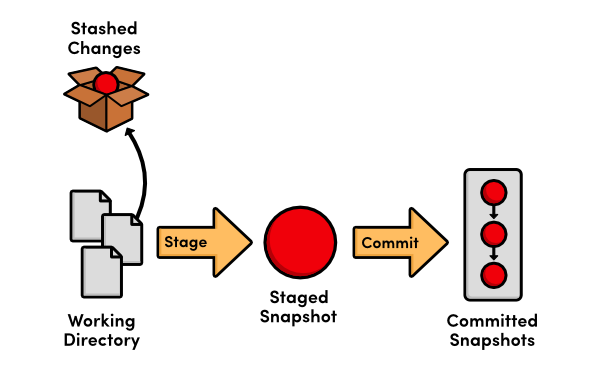
\includegraphics[keepaspectratio]{img/07_Stash/ejemplo-stash.png}}

Es importante no abusar del Stash ya que, aunque se puede etiquetar la informacion almacenada allí, es muy fácil olvidar que cambios le corresponden a cada ubicación sobre la que se está trabajando. Lo más recomendable es apoyarse en el uso de las ramas y, en caso de requerir el uso del Stash, recuperar esos cambios almacenados lo antes posible y continuar con el trabajo donde se dejó, en lugar de mantenerlo pendiente.

\pandocbounded{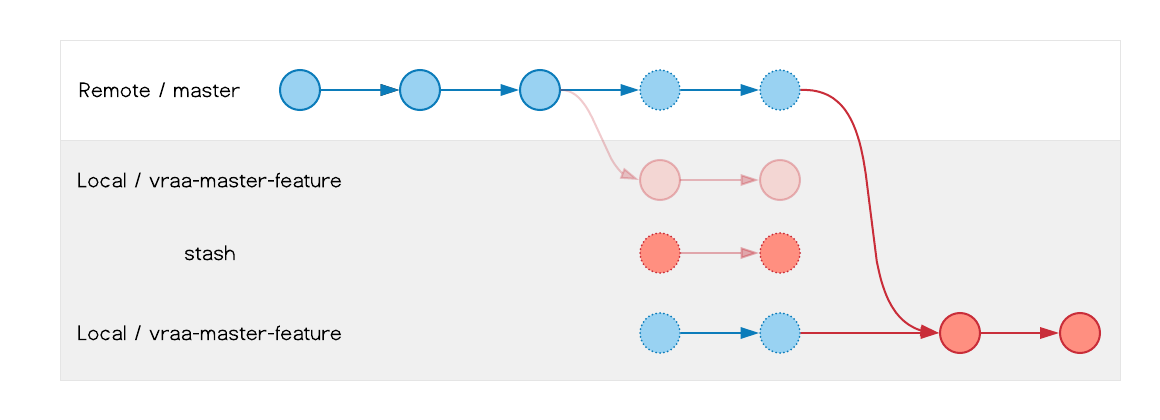
\includegraphics[keepaspectratio]{img/07_Stash/ejemplo-stash-1.png}}

Imagina que \textbf{Tony Stark} está mejorando su armadura en su taller, pero de repente recibe una alerta de \textbf{SHIELD} porque \textbf{Thanos} está atacando. No puede seguir trabajando en su traje en ese momento, pero tampoco quiere \emph{perder sus avances}, así que \emph{guarda} todas sus modificaciones en un compartimento seguro de su laboratorio para \emph{retomarlas más tarde}.

En Git, el \texttt{stash} funciona igual: si estás trabajando en cambios pero necesitas cambiar de rama o atender otra tarea sin perder tu progreso, puedes \emph{``guardarlos''} temporalmente con \texttt{git\ stash} y recuperarlos después con \texttt{git\ stash\ pop} o \texttt{git\ stash\ apply}.

\section{El Stash}\label{el-stash}

Supongamos que Iron Man, Thor, Hulk y Black Widow terminan sus misiones de alta prioridad, por lo que estas se remueven de sus respectivos registros:

\begin{itemize}
\tightlist
\item
  Iron Man
\end{itemize}

\begin{Shaded}
\begin{Highlighting}[]
\CommentTok{\# Misiones de Iron Man}

\ExtensionTok{1.} \PreprocessorTok{**}\NormalTok{Desarrollar el Mark XLVII}\PreprocessorTok{**}

   \ExtensionTok{{-}}\NormalTok{ Descripción: Implementar mejoras en el sistema de vuelo y armas del nuevo traje.}
   \ExtensionTok{{-}}\NormalTok{ Prioridad: Media}
   \ExtensionTok{{-}}\NormalTok{ Fecha límite: 2025{-}02{-}15}
\end{Highlighting}
\end{Shaded}

\begin{itemize}
\tightlist
\item
  Thor
\end{itemize}

\begin{Shaded}
\begin{Highlighting}[]
\CommentTok{\# Misiones de Thor}

\ExtensionTok{1.} \PreprocessorTok{**}\NormalTok{Negociar una alianza con los Elfos Oscuros}\PreprocessorTok{**}
   \ExtensionTok{{-}}\NormalTok{ Descripción: Organizar un tratado de paz para evitar conflictos en los Nueve Reinos.}
   \ExtensionTok{{-}}\NormalTok{ Prioridad: Media}
   \ExtensionTok{{-}}\NormalTok{ Fecha límite: 2025{-}03{-}01}
\end{Highlighting}
\end{Shaded}

\begin{itemize}
\tightlist
\item
  Hulk
\end{itemize}

\begin{Shaded}
\begin{Highlighting}[]
\CommentTok{\# Misiones de Hulk}

\ExtensionTok{1.} \PreprocessorTok{**}\NormalTok{Probar nuevos métodos de control}\PreprocessorTok{**}

   \ExtensionTok{{-}}\NormalTok{ Descripción: Colaborar con Bruce Banner para mejorar la técnica de meditación bajo estrés.}
   \ExtensionTok{{-}}\NormalTok{ Prioridad: Media}
   \ExtensionTok{{-}}\NormalTok{ Fecha límite: 2025{-}02{-}05}
\end{Highlighting}
\end{Shaded}

\begin{itemize}
\tightlist
\item
  Black Widow
\end{itemize}

\begin{Shaded}
\begin{Highlighting}[]
\CommentTok{\# Misiones de Black Widow}

\ExtensionTok{1.} \PreprocessorTok{**}\NormalTok{Entrenar a nuevos reclutas de SHIELD}\PreprocessorTok{**}

   \ExtensionTok{{-}}\NormalTok{ Descripción: Liderar sesiones avanzadas de combate y estrategias de infiltración.}
   \ExtensionTok{{-}}\NormalTok{ Prioridad: Media}
   \ExtensionTok{{-}}\NormalTok{ Fecha límite: 2025{-}02{-}15}
\end{Highlighting}
\end{Shaded}

\begin{Shaded}
\begin{Highlighting}[]
\FunctionTok{git}\NormalTok{ commit }\AttributeTok{{-}am} \StringTok{"cumplimiento misiones alta prioridad: Iron Man, Thor, Hulk, Black Widow"}
\end{Highlighting}
\end{Shaded}

\begin{Shaded}
\begin{Highlighting}[]
\ExtensionTok{[main}\NormalTok{ e4c626a] cumplimiento misiones alta prioridad: Iron Man, Thor, Hulk, Black Widow}
 \ExtensionTok{4}\NormalTok{ files changed, 4 insertions}\ErrorTok{(}\ExtensionTok{+}\KeywordTok{)}\ExtensionTok{,}\NormalTok{ 49 deletions}\ErrorTok{(}\ExtensionTok{{-}}\KeywordTok{)}
\end{Highlighting}
\end{Shaded}

Se consideran nuevas misiones para asignar a estos héroes, estas deben agregarse a sus registros:

\begin{itemize}
\tightlist
\item
  Iron Man
\end{itemize}

\begin{Shaded}
\begin{Highlighting}[]
\CommentTok{\# Misiones de Iron Man}

\ExtensionTok{1.} \PreprocessorTok{**}\NormalTok{Desarrollar el Mark XLVII}\PreprocessorTok{**}

   \ExtensionTok{{-}}\NormalTok{ Descripción: Implementar mejoras en el sistema de vuelo y armas del nuevo traje.}
   \ExtensionTok{{-}}\NormalTok{ Prioridad: Media}
   \ExtensionTok{{-}}\NormalTok{ Fecha límite: 2025{-}02{-}15}

\ExtensionTok{2.} \PreprocessorTok{**}\NormalTok{Desactivar un satélite fuera de control}\PreprocessorTok{**}

   \ExtensionTok{{-}}\NormalTok{ Descripción: Un satélite experimental de Stark Industries ha sido hackeado y está a punto de impactar contra una ciudad. Debe ser desactivado antes de que cause una catástrofe.}
   \ExtensionTok{{-}}\NormalTok{ Prioridad: Alta}
   \ExtensionTok{{-}}\NormalTok{ Fecha límite: 2025{-}03{-}15}

\ExtensionTok{3.} \PreprocessorTok{**}\NormalTok{Recuperar una armadura robada}\PreprocessorTok{**}

   \ExtensionTok{{-}}\NormalTok{ Descripción: Un prototipo del traje Mark L ha sido robado y modificado con tecnología avanzada. Se debe recuperar antes de que caiga en las manos equivocadas.}
   \ExtensionTok{{-}}\NormalTok{ Prioridad: Alta}
   \ExtensionTok{{-}}\NormalTok{ Fecha límite: 2025{-}02{-}28}
\end{Highlighting}
\end{Shaded}

\begin{itemize}
\tightlist
\item
  Thor
\end{itemize}

\begin{Shaded}
\begin{Highlighting}[]
\CommentTok{\# Misiones de Thor}

\ExtensionTok{1.} \PreprocessorTok{**}\NormalTok{Negociar una alianza con los Elfos Oscuros}\PreprocessorTok{**}
   \ExtensionTok{{-}}\NormalTok{ Descripción: Organizar un tratado de paz para evitar conflictos en los Nueve Reinos.}
   \ExtensionTok{{-}}\NormalTok{ Prioridad: Media}
   \ExtensionTok{{-}}\NormalTok{ Fecha límite: 2025{-}03{-}01}

\ExtensionTok{2.} \PreprocessorTok{**}\NormalTok{Defender el Bifrost de un ataque enemigo}\PreprocessorTok{**}

   \ExtensionTok{{-}}\NormalTok{ Descripción: Un ejército de Jotuns ha intentado invadir Asgard usando el Bifrost. Es necesario repeler la invasión y sellar el portal.}
   \ExtensionTok{{-}}\NormalTok{ Prioridad: Alta}
   \ExtensionTok{{-}}\NormalTok{ Fecha límite: 2025{-}02{-}20}

\ExtensionTok{3.} \PreprocessorTok{**}\NormalTok{Capturar a Loki antes de su próximo golpe}\PreprocessorTok{**}

   \ExtensionTok{{-}}\NormalTok{ Descripción: Loki ha escapado de Asgard y planea sembrar el caos en la Tierra. Se debe localizar y capturarlo antes de que su plan se complete.}
   \ExtensionTok{{-}}\NormalTok{ Prioridad: Alta}
   \ExtensionTok{{-}}\NormalTok{ Fecha límite: 2025{-}03{-}05}
\end{Highlighting}
\end{Shaded}

\begin{itemize}
\tightlist
\item
  Hulk
\end{itemize}

\begin{Shaded}
\begin{Highlighting}[]
\CommentTok{\# Misiones de Hulk}

\ExtensionTok{1.} \PreprocessorTok{**}\NormalTok{Probar nuevos métodos de control}\PreprocessorTok{**}

   \ExtensionTok{{-}}\NormalTok{ Descripción: Colaborar con Bruce Banner para mejorar la técnica de meditación bajo estrés.}
   \ExtensionTok{{-}}\NormalTok{ Prioridad: Media}
   \ExtensionTok{{-}}\NormalTok{ Fecha límite: 2025{-}02{-}05}

\ExtensionTok{2.} \PreprocessorTok{**}\NormalTok{Detener a un Hulk Rojo descontrolado}\PreprocessorTok{**}

   \ExtensionTok{{-}}\NormalTok{ Descripción: Un experimento fallido ha causado que un nuevo Hulk Rojo entre en frenesí. Se debe detener antes de que destruya una ciudad entera.}
   \ExtensionTok{{-}}\NormalTok{ Prioridad: Alta}
   \ExtensionTok{{-}}\NormalTok{ Fecha límite: 2025{-}02{-}25}

\ExtensionTok{3.} \PreprocessorTok{**}\NormalTok{Evitar la activación de un ejército de Hulks sintéticos}\PreprocessorTok{**}

   \ExtensionTok{{-}}\NormalTok{ Descripción: Un grupo de científicos ha clonado células Gamma para crear supersoldados. Se debe destruir la instalación y detener el proyecto.}
   \ExtensionTok{{-}}\NormalTok{ Prioridad: Alta}
   \ExtensionTok{{-}}\NormalTok{ Fecha límite: 2025{-}03{-}08}
\end{Highlighting}
\end{Shaded}

\begin{itemize}
\tightlist
\item
  Black Widow
\end{itemize}

\begin{Shaded}
\begin{Highlighting}[]
\CommentTok{\# Misiones de Black Widow}

\ExtensionTok{1.} \PreprocessorTok{**}\NormalTok{Entrenar a nuevos reclutas de SHIELD}\PreprocessorTok{**}

   \ExtensionTok{{-}}\NormalTok{ Descripción: Liderar sesiones avanzadas de combate y estrategias de infiltración.}
   \ExtensionTok{{-}}\NormalTok{ Prioridad: Media}
   \ExtensionTok{{-}}\NormalTok{ Fecha límite: 2025{-}02{-}15}

\ExtensionTok{2.} \PreprocessorTok{**}\NormalTok{Interceptar un cargamento de armas biológicas}\PreprocessorTok{**}

   \ExtensionTok{{-}}\NormalTok{ Descripción: Un grupo terrorista ha conseguido armas biológicas de última generación. Se debe interceptar el cargamento antes de que sea distribuido.}
   \ExtensionTok{{-}}\NormalTok{ Prioridad: Alta}
   \ExtensionTok{{-}}\NormalTok{ Fecha límite: 2025{-}02{-}22}

\ExtensionTok{3.} \PreprocessorTok{**}\NormalTok{Eliminar una célula de la Mano en Nueva York}\PreprocessorTok{**}

   \ExtensionTok{{-}}\NormalTok{ Descripción: Se ha detectado actividad de la organización secreta La Mano en Nueva York. Se debe infiltrar su base y desmantelar sus operaciones.}
   \ExtensionTok{{-}}\NormalTok{ Prioridad: Alta}
   \ExtensionTok{{-}}\NormalTok{ Fecha límite: 2025{-}03{-}10}
\end{Highlighting}
\end{Shaded}

Pero antes de completar la asignación de las nuevas misiones llega el Capitán América para registrarse:

\begin{enumerate}
\def\labelenumi{\arabic{enumi}.}
\tightlist
\item
  Primero guardamos las asignaciones en el \texttt{stash} para no perder esa información.
\end{enumerate}

\begin{Shaded}
\begin{Highlighting}[]
\FunctionTok{git}\NormalTok{ stash}
\end{Highlighting}
\end{Shaded}

\begin{Shaded}
\begin{Highlighting}[]
\ExtensionTok{Directorio}\NormalTok{ de trabajo y estado de índice WIP on main: e4c626a cumplimiento misiones alta prioridad: Iron Man, Thor, Hulk, Black Widow guardados}
\end{Highlighting}
\end{Shaded}

Puedes notar que al ver el estado del repositorio, git no muestra cambios en los archivos.

\begin{Shaded}
\begin{Highlighting}[]
\FunctionTok{git}\NormalTok{ s}
\end{Highlighting}
\end{Shaded}

\begin{Shaded}
\begin{Highlighting}[]
\CommentTok{\#\# main}
\end{Highlighting}
\end{Shaded}

\begin{enumerate}
\def\labelenumi{\arabic{enumi}.}
\setcounter{enumi}{1}
\tightlist
\item
  Hacemos el registro del Capitán América.
\end{enumerate}

\begin{itemize}
\tightlist
\item
  \texttt{descripciones.md}
\end{itemize}

\begin{Shaded}
\begin{Highlighting}[]
\CommentTok{\#\# Capitán América}

\ExtensionTok{{-}} \PreprocessorTok{**}\NormalTok{Nombre real:}\PreprocessorTok{**}\NormalTok{ Steve Rogers}
\ExtensionTok{{-}} \PreprocessorTok{**}\NormalTok{Descripción:}\PreprocessorTok{**}\NormalTok{ Un supersoldado con habilidades físicas mejoradas, líder nato y defensor de la justicia.}
\end{Highlighting}
\end{Shaded}

\begin{itemize}
\tightlist
\item
  \texttt{origenes.md}
\end{itemize}

\begin{Shaded}
\begin{Highlighting}[]
\CommentTok{\#\# Capitán América}

\ExtensionTok{{-}}\NormalTok{ Fue seleccionado para el Proyecto Súper Soldado durante la Segunda Guerra Mundial y recibió el Suero del Supersoldado.}
\ExtensionTok{{-}}\NormalTok{ Tras liderar varias misiones contra HYDRA, quedó congelado en el hielo por décadas hasta ser encontrado por SHIELD.}
\end{Highlighting}
\end{Shaded}

\begin{itemize}
\tightlist
\item
  \texttt{debilidades.md}
\end{itemize}

\begin{Shaded}
\begin{Highlighting}[]
\CommentTok{\#\# Capitán América}

\ExtensionTok{{-}}\NormalTok{ A pesar de su fuerza mejorada, sigue siendo humano y vulnerable a heridas graves.}
\ExtensionTok{{-}}\NormalTok{ Su código moral a veces interfiere con decisiones estratégicas difíciles.}
\end{Highlighting}
\end{Shaded}

\begin{itemize}
\tightlist
\item
  \texttt{misiones/capitan\_america.md}
\end{itemize}

\begin{Shaded}
\begin{Highlighting}[]
\CommentTok{\# Misiones de Capitán América}

\ExtensionTok{1.} \PreprocessorTok{**}\NormalTok{Supervisar el entrenamiento de nuevos Vengadores}\PreprocessorTok{**}
   \ExtensionTok{{-}}\NormalTok{ Descripción: Dirigir ejercicios tácticos y sesiones de combate para nuevos reclutas.}
   \ExtensionTok{{-}}\NormalTok{ Prioridad: Media}
   \ExtensionTok{{-}}\NormalTok{ Fecha límite: 2025{-}02{-}10}

\ExtensionTok{2.} \PreprocessorTok{**}\NormalTok{Recuperar el Escudo original}\PreprocessorTok{**}
   \ExtensionTok{{-}}\NormalTok{ Descripción: Investigar la ubicación del escudo original, extraviado tras la batalla contra Thanos.}
   \ExtensionTok{{-}}\NormalTok{ Prioridad: Alta}
   \ExtensionTok{{-}}\NormalTok{ Fecha límite: 2025{-}01{-}28}

\ExtensionTok{3.} \PreprocessorTok{**}\NormalTok{Desmantelar células de HYDRA en Sudamérica}\PreprocessorTok{**}
   \ExtensionTok{{-}}\NormalTok{ Descripción: Operación encubierta para identificar y neutralizar bases secretas de HYDRA.}
   \ExtensionTok{{-}}\NormalTok{ Prioridad: Alta}
   \ExtensionTok{{-}}\NormalTok{ Fecha límite: 2025{-}02{-}15}
\end{Highlighting}
\end{Shaded}

\begin{itemize}
\tightlist
\item
  \texttt{README.md}
\end{itemize}

\begin{Shaded}
\begin{Highlighting}[]
\ExtensionTok{{-}}\NormalTok{ [capitan america]}\ErrorTok{(}\ExtensionTok{/misiones/capitan\_america.md}\KeywordTok{)}
\end{Highlighting}
\end{Shaded}

\begin{enumerate}
\def\labelenumi{\arabic{enumi}.}
\setcounter{enumi}{2}
\tightlist
\item
  guardamos el registro del Capitán América
\end{enumerate}

\begin{Shaded}
\begin{Highlighting}[]
\FunctionTok{git}\NormalTok{ commit }\AttributeTok{{-}m} \StringTok{"se une Capitan America"}
\end{Highlighting}
\end{Shaded}

\begin{Shaded}
\begin{Highlighting}[]
\ExtensionTok{[main}\NormalTok{ 5319e68] se une Capitan America}
 \ExtensionTok{5}\NormalTok{ files changed, 34 insertions}\ErrorTok{(}\ExtensionTok{+}\KeywordTok{)}
 \ExtensionTok{create}\NormalTok{ mode 100644 misiones/capitan\_america.md}
\end{Highlighting}
\end{Shaded}

\begin{enumerate}
\def\labelenumi{\arabic{enumi}.}
\setcounter{enumi}{3}
\tightlist
\item
  para poder continuar con la asignación de nuevas misiones, tenemos que recuperarlas del \texttt{stash}. Para ello, antes que otra cosa, debemos listar todo lo que se haya guardado en el \texttt{stash}.
\end{enumerate}

\begin{Shaded}
\begin{Highlighting}[]
\FunctionTok{git}\NormalTok{ stash list}
\end{Highlighting}
\end{Shaded}

\begin{Shaded}
\begin{Highlighting}[]
\ExtensionTok{stash@\{0\}:}\NormalTok{ WIP on main: e4c626a cumplimiento misiones alta prioridad: Iron Man, Thor, Hulk, Black Widow}
\end{Highlighting}
\end{Shaded}

Este mensaje contiene bastante información:

\begin{itemize}
\item
  \texttt{stash@\{0\}} indica el lugar, en jerarquía, del trabajo, en este caso es \texttt{0}.
\item
  \texttt{WIP} Work In Progres.
\item
  \texttt{on\ main} indica la rama en la que se encuentra el trabajo \texttt{main}.
\item
  \texttt{e4c626a\ cumplimiento\ misiones\ alta\ prioridad:\ Iron\ Man,\ Thor,\ Hulk,\ Black\ Widow} indica el registro sobre el que se estaba trabajando.
\end{itemize}

Para recuperar nuestro trabajo pendiente, la asignación de nuevas misiones, empleamos el siguiente comando.

\begin{Shaded}
\begin{Highlighting}[]
\FunctionTok{git}\NormalTok{ stash pop stash@}\DataTypeTok{\textbackslash{}\{}\NormalTok{0}\DataTypeTok{\textbackslash{}\}}
\end{Highlighting}
\end{Shaded}

\begin{Shaded}
\begin{Highlighting}[]
\ExtensionTok{En}\NormalTok{ la rama main}
\ExtensionTok{Cambios}\NormalTok{ no rastreados para el commit:}
  \KeywordTok{(}\ExtensionTok{usa} \StringTok{"git add \textless{}archivo\textgreater{}..."}\NormalTok{ para actualizar lo que será confirmado}\KeywordTok{)}
  \KeywordTok{(}\ExtensionTok{usa} \StringTok{"git restore \textless{}archivo\textgreater{}..."}\NormalTok{ para descartar los cambios en el directorio de trabajo}\KeywordTok{)}
    \ExtensionTok{modificados:}\NormalTok{     misiones/black\_widow.md}
    \ExtensionTok{modificados:}\NormalTok{     misiones/hulk.md}
    \ExtensionTok{modificados:}\NormalTok{     misiones/iron\_man.md}
    \ExtensionTok{modificados:}\NormalTok{     misiones/thor.md}

\ExtensionTok{sin}\NormalTok{ cambios agregados al commit }\ErrorTok{(}\ExtensionTok{usa} \StringTok{"git add"}\NormalTok{ y/o }\StringTok{"git commit {-}a"}\KeywordTok{)}
\ExtensionTok{Descartado}\NormalTok{ stash@\{0\} }\ErrorTok{(}\ExtensionTok{f24e0582315c5541a0d8fddc35862e34e1242e15}\KeywordTok{)}
\end{Highlighting}
\end{Shaded}

Con \texttt{stash@\textbackslash{}\{0\textbackslash{}\}} indicamos cual es el trabajo que queremos recuperar, en este caso era el \texttt{0}; para este particular caso, también podemos emplear \texttt{git\ stash\ pop} ya que por defecto devuelve el trabajo en la posicion \texttt{0} y el resto los sube un lugar.

Comprovamos el estado del repositorio.

\begin{Shaded}
\begin{Highlighting}[]
\FunctionTok{git}\NormalTok{ s}
\end{Highlighting}
\end{Shaded}

\begin{Shaded}
\begin{Highlighting}[]
\CommentTok{\#\# main}
 \ExtensionTok{M}\NormalTok{ misiones/black\_widow.md}
 \ExtensionTok{M}\NormalTok{ misiones/hulk.md}
 \ExtensionTok{M}\NormalTok{ misiones/iron\_man.md}
 \ExtensionTok{M}\NormalTok{ misiones/thor.md}
\end{Highlighting}
\end{Shaded}

Tenemos el trabajo pendiente de vuelta, por lo que podemos seguir trabajando en la asignación de misiones nuevas.

\section{Conflictos en el Stash}\label{conflictos-en-el-stash}

\begin{enumerate}
\def\labelenumi{\arabic{enumi}.}
\tightlist
\item
  Antes de confirmar la asignación de las nuevas misiones, Visión llega para registrarse por lo que, de nuevo, guardamos el progreso en el \texttt{stash}.
\end{enumerate}

\begin{Shaded}
\begin{Highlighting}[]
\FunctionTok{git}\NormalTok{ stash}
\end{Highlighting}
\end{Shaded}

\begin{Shaded}
\begin{Highlighting}[]
\ExtensionTok{Directorio}\NormalTok{ de trabajo y estado de índice WIP on main: 5319e68 se une Capitan America guardados}
\end{Highlighting}
\end{Shaded}

\begin{enumerate}
\def\labelenumi{\arabic{enumi}.}
\setcounter{enumi}{1}
\tightlist
\item
  Hacemos el registro de Visión.
\end{enumerate}

\begin{itemize}
\tightlist
\item
  \texttt{descripciones.md}
\end{itemize}

\begin{Shaded}
\begin{Highlighting}[]
\CommentTok{\#\# Visión}

\ExtensionTok{{-}} \PreprocessorTok{**}\NormalTok{Nombre real:}\PreprocessorTok{**}\NormalTok{ Visión}
\ExtensionTok{{-}} \PreprocessorTok{**}\NormalTok{Descripción:}\PreprocessorTok{**}\NormalTok{ Sintético avanzado creado con la Gema de la Mente y el cuerpo diseñado por Ultron. Posee inteligencia artificial altamente evolucionada y habilidades de manipulación de densidad.}
\end{Highlighting}
\end{Shaded}

\begin{itemize}
\tightlist
\item
  \texttt{origenes.md}
\end{itemize}

\begin{Shaded}
\begin{Highlighting}[]
\CommentTok{\#\# Visión}

\ExtensionTok{{-}}\NormalTok{ Fue creado por Ultron con el propósito de ser su cuerpo definitivo, pero obtuvo libre albedrío gracias a la intervención de Tony Stark, Bruce Banner y Thor.}
\ExtensionTok{{-}}\NormalTok{ La Gema de la Mente le otorga habilidades extraordinarias, incluyendo vuelo, manipulación de densidad y un intelecto superior.}
\end{Highlighting}
\end{Shaded}

\begin{itemize}
\tightlist
\item
  \texttt{debilidades.md}
\end{itemize}

\begin{Shaded}
\begin{Highlighting}[]
\CommentTok{\#\# Visión}

\ExtensionTok{{-}}\NormalTok{ Su conexión con la Gema de la Mente lo hace vulnerable si esta es removida o dañada.}
\ExtensionTok{{-}}\NormalTok{ Puede ser afectado por ataques de manipulación de sistemas o tecnología avanzada.}
\end{Highlighting}
\end{Shaded}

\begin{itemize}
\tightlist
\item
  \texttt{misiones/vision.md}
\end{itemize}

\begin{Shaded}
\begin{Highlighting}[]
\CommentTok{\# Misiones de Visión}

\ExtensionTok{1.} \PreprocessorTok{**}\NormalTok{Analizar anomalías en la Gema de la Mente}\PreprocessorTok{**}  
   \ExtensionTok{{-}} \PreprocessorTok{**}\NormalTok{Descripción:}\PreprocessorTok{**}\NormalTok{ Examinar irregularidades en la Gema de la Mente para prevenir inestabilidades.  }
   \ExtensionTok{{-}} \PreprocessorTok{**}\NormalTok{Prioridad:}\PreprocessorTok{**}\NormalTok{ Alta  }
   \ExtensionTok{{-}} \PreprocessorTok{**}\NormalTok{Fecha límite:}\PreprocessorTok{**}\NormalTok{ 2025{-}02{-}05  }

\ExtensionTok{2.} \PreprocessorTok{**}\NormalTok{Actualizar protocolos de defensa en la Torre de los Vengadores}\PreprocessorTok{**}  
   \ExtensionTok{{-}} \PreprocessorTok{**}\NormalTok{Descripción:}\PreprocessorTok{**}\NormalTok{ Optimizar los sistemas de seguridad y detección de amenazas.  }
   \ExtensionTok{{-}} \PreprocessorTok{**}\NormalTok{Prioridad:}\PreprocessorTok{**}\NormalTok{ Media  }
   \ExtensionTok{{-}} \PreprocessorTok{**}\NormalTok{Fecha límite:}\PreprocessorTok{**}\NormalTok{ 2025{-}02{-}15  }

\ExtensionTok{3.} \PreprocessorTok{**}\NormalTok{Proteger a Wanda Maximoff de amenazas externas}\PreprocessorTok{**}  
   \ExtensionTok{{-}} \PreprocessorTok{**}\NormalTok{Descripción:}\PreprocessorTok{**}\NormalTok{ Vigilar e intervenir en caso de ataques dirigidos contra Scarlet Witch.  }
   \ExtensionTok{{-}} \PreprocessorTok{**}\NormalTok{Prioridad:}\PreprocessorTok{**}\NormalTok{ Alta  }
   \ExtensionTok{{-}} \PreprocessorTok{**}\NormalTok{Fecha límite:}\PreprocessorTok{**}\NormalTok{ 2025{-}01{-}30  }
\end{Highlighting}
\end{Shaded}

\begin{itemize}
\tightlist
\item
  \texttt{README.md}
\end{itemize}

\begin{Shaded}
\begin{Highlighting}[]
\ExtensionTok{{-}} \PreprocessorTok{[}\SpecialStringTok{vision}\PreprocessorTok{]}\ErrorTok{(}\ExtensionTok{/misiones/vision.md}\KeywordTok{)}
\end{Highlighting}
\end{Shaded}

\begin{enumerate}
\def\labelenumi{\arabic{enumi}.}
\setcounter{enumi}{2}
\tightlist
\item
  guardamos el registro de Visión
\end{enumerate}

\begin{Shaded}
\begin{Highlighting}[]
\FunctionTok{git}\NormalTok{ commit }\AttributeTok{{-}m} \StringTok{"se une Vision"}
\end{Highlighting}
\end{Shaded}

\begin{Shaded}
\begin{Highlighting}[]
\ExtensionTok{[main}\NormalTok{ 8531ef2] se une Vision}
 \ExtensionTok{5}\NormalTok{ files changed, 34 insertions}\ErrorTok{(}\ExtensionTok{+}\KeywordTok{)}
 \ExtensionTok{create}\NormalTok{ mode 100644 misiones/vision.md}
\end{Highlighting}
\end{Shaded}

\begin{enumerate}
\def\labelenumi{\arabic{enumi}.}
\setcounter{enumi}{3}
\tightlist
\item
  Mientras se registraba a Visión, llegó una misión de extrema urgencia, la cual tomó Iron Man, por lo que se agrega a su registro de misiones como una nueva asignación.
\end{enumerate}

\begin{itemize}
\tightlist
\item
  \texttt{misiones/iron\_man.md}
\end{itemize}

\begin{Shaded}
\begin{Highlighting}[]
\CommentTok{\# Misiones de Iron Man}

\ExtensionTok{1.} \PreprocessorTok{**}\NormalTok{Desarrollar el Mark XLVII}\PreprocessorTok{**}

   \ExtensionTok{{-}}\NormalTok{ Descripción: Implementar mejoras en el sistema de vuelo y armas del nuevo traje.}
   \ExtensionTok{{-}}\NormalTok{ Prioridad: Media}
   \ExtensionTok{{-}}\NormalTok{ Fecha límite: 2025{-}02{-}15}

\ExtensionTok{2.} \PreprocessorTok{**}\NormalTok{Proteger a un testigo clave en un juicio internacional}\PreprocessorTok{**}

   \ExtensionTok{{-}}\NormalTok{ Descripción: Vigilar y garantizar la seguridad de un testigo protegido que posee información vital sobre una red de espionaje criminal.}
   \ExtensionTok{{-}}\NormalTok{ Prioridad: Alta}
   \ExtensionTok{{-}}\NormalTok{ Fecha límite: 2025{-}02{-}12}
\end{Highlighting}
\end{Shaded}

\begin{enumerate}
\def\labelenumi{\arabic{enumi}.}
\setcounter{enumi}{4}
\tightlist
\item
  Se registra la nueva asignación.
\end{enumerate}

\begin{Shaded}
\begin{Highlighting}[]
\FunctionTok{git}\NormalTok{ commit }\AttributeTok{{-}am} \StringTok{"asignacion de emergencia para Iron Man"}
\end{Highlighting}
\end{Shaded}

\begin{Shaded}
\begin{Highlighting}[]
\ExtensionTok{[main}\NormalTok{ b307d16] asignacion de emergencia para Iron Man}
 \ExtensionTok{1}\NormalTok{ file changed, 6 insertions}\ErrorTok{(}\ExtensionTok{+}\KeywordTok{)}
\end{Highlighting}
\end{Shaded}

\begin{enumerate}
\def\labelenumi{\arabic{enumi}.}
\setcounter{enumi}{5}
\tightlist
\item
  Se retoma la asignación de nuevas misiones.
\end{enumerate}

\begin{Shaded}
\begin{Highlighting}[]
\FunctionTok{git}\NormalTok{ stash pop }
\end{Highlighting}
\end{Shaded}

\begin{Shaded}
\begin{Highlighting}[]
\ExtensionTok{Auto{-}fusionando}\NormalTok{ misiones/iron\_man.md}
\ExtensionTok{CONFLICTO} \ErrorTok{(}\ExtensionTok{contenido}\KeywordTok{)}\BuiltInTok{:}\NormalTok{ Conflicto de fusión en misiones/iron\_man.md}
\ExtensionTok{En}\NormalTok{ la rama main}
\ExtensionTok{Cambios}\NormalTok{ a ser confirmados:}
  \KeywordTok{(}\ExtensionTok{usa} \StringTok{"git restore {-}{-}staged \textless{}archivo\textgreater{}..."}\NormalTok{ para sacar del área de stage}\KeywordTok{)}
    \ExtensionTok{modificados:}\NormalTok{     misiones/black\_widow.md}
    \ExtensionTok{modificados:}\NormalTok{     misiones/hulk.md}
    \ExtensionTok{modificados:}\NormalTok{     misiones/thor.md}

\ExtensionTok{Rutas}\NormalTok{ no fusionadas:}
  \KeywordTok{(}\ExtensionTok{usa} \StringTok{"git restore {-}{-}staged \textless{}archivo\textgreater{}..."}\NormalTok{ para sacar del área de stage}\KeywordTok{)}
  \KeywordTok{(}\ExtensionTok{usa} \StringTok{"git add \textless{}archivo\textgreater{}..."}\NormalTok{ para marcar una resolución}\KeywordTok{)}
    \ExtensionTok{modificados}\NormalTok{ por ambos:  misiones/iron\_man.md}

\ExtensionTok{La}\NormalTok{ entrada de stash se guardó en caso de ser necesario nuevamente.}
\end{Highlighting}
\end{Shaded}

\begin{enumerate}
\def\labelenumi{\arabic{enumi}.}
\setcounter{enumi}{6}
\item
  Nos hemos encontrado con un conflicto en las misiones de Iron Man.
\item
  Comprobamos el estado del repositorio.
\end{enumerate}

\begin{Shaded}
\begin{Highlighting}[]
\FunctionTok{git}\NormalTok{ s}
\end{Highlighting}
\end{Shaded}

\begin{Shaded}
\begin{Highlighting}[]
\CommentTok{\#\# main}
\ExtensionTok{M}\NormalTok{  misiones/black\_widow.md}
\ExtensionTok{M}\NormalTok{  misiones/hulk.md}
\ExtensionTok{UU}\NormalTok{ misiones/iron\_man.md}
\ExtensionTok{M}\NormalTok{  misiones/thor.md}
\end{Highlighting}
\end{Shaded}

Git reconoce las modificaciones en las misiones de Thor, Hulk y Black Widow; el marcador \texttt{UU} indica que se realizaron cambios desde ambos lados del \texttt{stash}

\begin{enumerate}
\def\labelenumi{\arabic{enumi}.}
\setcounter{enumi}{8}
\tightlist
\item
  Resolvemos los conflictos encontrados.
\end{enumerate}

\begin{itemize}
\tightlist
\item
  \texttt{misiones/iron\_man.md}
\end{itemize}

\begin{Shaded}
\begin{Highlighting}[]
\CommentTok{\# Misiones de Iron Man}

\ExtensionTok{1.} \PreprocessorTok{**}\NormalTok{Desarrollar el Mark XLVII}\PreprocessorTok{**}
   
   \ExtensionTok{{-}}\NormalTok{ Descripción: Implementar mejoras en el sistema de vuelo y armas del nuevo traje.}
   \ExtensionTok{{-}}\NormalTok{ Prioridad: Media}
   \ExtensionTok{{-}}\NormalTok{ Fecha límite: 2025{-}02{-}15}

\OperatorTok{\textless{}\textless{}\textless{}\textless{}\textless{}\textless{}\textless{}}\NormalTok{ Updated }\ExtensionTok{upstream}
\ExtensionTok{2.} \PreprocessorTok{**}\NormalTok{Proteger a un testigo clave en un juicio internacional}\PreprocessorTok{**}

   \ExtensionTok{{-}}\NormalTok{ Descripción: Vigilar y garantizar la seguridad de un testigo protegido que posee información vital sobre una red de espionaje criminal.}
   \ExtensionTok{{-}}\NormalTok{ Prioridad: Alta}
   \ExtensionTok{{-}}\NormalTok{ Fecha límite: 2025{-}03{-}12}
\ExtensionTok{=======}
\ExtensionTok{2.} \PreprocessorTok{**}\NormalTok{Desactivar un satélite fuera de control}\PreprocessorTok{**}
   
   \ExtensionTok{{-}}\NormalTok{ Descripción: Un satélite experimental de Stark Industries ha sido hackeado y está a punto de impactar contra una ciudad. Debe ser desactivado antes de que cause una catástrofe.}
   \ExtensionTok{{-}}\NormalTok{ Prioridad: Alta}
   \ExtensionTok{{-}}\NormalTok{ Fecha límite: 2025{-}03{-}15}

\ExtensionTok{3.} \PreprocessorTok{**}\NormalTok{Recuperar una armadura robada}\PreprocessorTok{**}
   
   \ExtensionTok{{-}}\NormalTok{ Descripción: Un prototipo del traje Mark L ha sido robado y modificado con tecnología avanzada. Se debe recuperar antes de que caiga en las manos equivocadas.}
   \ExtensionTok{{-}}\NormalTok{ Prioridad: Alta}
   \ExtensionTok{{-}}\NormalTok{ Fecha límite: 2025{-}02{-}28}
\OperatorTok{\textgreater{}\textgreater{}\textgreater{}\textgreater{}\textgreater{}\textgreater{}\textgreater{}}\NormalTok{ Stashed }\ExtensionTok{changes}
\end{Highlighting}
\end{Shaded}

Similarmente a los conflictos al mezclar ramas:

\begin{itemize}
\item
  La marca \texttt{\textless{}\textless{}\textless{}\textless{}\textless{}\textless{}\textless{}\ Updated\ upstream} indica el trabajo registrado desde el commit del que se guardó el trabajo en el \texttt{stash}.
\item
  La marca \texttt{=======} separa los trabajos del registro y del \texttt{stash}.
\item
  La marca \texttt{\textgreater{}\textgreater{}\textgreater{}\textgreater{}\textgreater{}\textgreater{}\textgreater{}\ Stashed\ changes} indica el trabajo almacenado en el \texttt{stash}.
\end{itemize}

En resumen lo que se encuentra entre \texttt{\textless{}\textless{}\textless{}\textless{}\textless{}\textless{}\textless{}\ Updated\ upstream} y \texttt{=======} es el trabajo registrado desde el commit en el que se almacenó el trabajo al \texttt{stash}; entre \texttt{=======} y \texttt{\textgreater{}\textgreater{}\textgreater{}\textgreater{}\textgreater{}\textgreater{}\textgreater{}\ tierra-65} se encuentra el trabajo almacenado en el \texttt{stash}.

\begin{enumerate}
\def\labelenumi{\arabic{enumi}.}
\setcounter{enumi}{9}
\tightlist
\item
  En este caso se mantendrán todas las misiones, solo se cambiará el número de misión.
\end{enumerate}

\begin{itemize}
\tightlist
\item
  \texttt{misiones/iron\_man.md}
\end{itemize}

\begin{Shaded}
\begin{Highlighting}[]
\CommentTok{\# Misiones de Iron Man}

\ExtensionTok{1.} \PreprocessorTok{**}\NormalTok{Desarrollar el Mark XLVII}\PreprocessorTok{**}
   
   \ExtensionTok{{-}}\NormalTok{ Descripción: Implementar mejoras en el sistema de vuelo y armas del nuevo traje.}
   \ExtensionTok{{-}}\NormalTok{ Prioridad: Media}
   \ExtensionTok{{-}}\NormalTok{ Fecha límite: 2025{-}02{-}15}

\ExtensionTok{2.} \PreprocessorTok{**}\NormalTok{Proteger a un testigo clave en un juicio internacional}\PreprocessorTok{**}

   \ExtensionTok{{-}}\NormalTok{ Descripción: Vigilar y garantizar la seguridad de un testigo protegido que posee información vital sobre una red de espionaje criminal.}
   \ExtensionTok{{-}}\NormalTok{ Prioridad: Alta}
   \ExtensionTok{{-}}\NormalTok{ Fecha límite: 2025{-}03{-}12}

\ExtensionTok{3.} \PreprocessorTok{**}\NormalTok{Desactivar un satélite fuera de control}\PreprocessorTok{**}
   
   \ExtensionTok{{-}}\NormalTok{ Descripción: Un satélite experimental de Stark Industries ha sido hackeado y está a punto de impactar contra una ciudad. Debe ser desactivado antes de que cause una catástrofe.}
   \ExtensionTok{{-}}\NormalTok{ Prioridad: Alta}
   \ExtensionTok{{-}}\NormalTok{ Fecha límite: 2025{-}03{-}15}

\ExtensionTok{4.} \PreprocessorTok{**}\NormalTok{Recuperar una armadura robada}\PreprocessorTok{**}
   
   \ExtensionTok{{-}}\NormalTok{ Descripción: Un prototipo del traje Mark L ha sido robado y modificado con tecnología avanzada. Se debe recuperar antes de que caiga en las manos equivocadas.}
   \ExtensionTok{{-}}\NormalTok{ Prioridad: Alta}
   \ExtensionTok{{-}}\NormalTok{ Fecha límite: 2025{-}02{-}28}
\end{Highlighting}
\end{Shaded}

\begin{enumerate}
\def\labelenumi{\arabic{enumi}.}
\setcounter{enumi}{10}
\tightlist
\item
  Registramos la asignación de nuevas misiones.
\end{enumerate}

\begin{Shaded}
\begin{Highlighting}[]
\FunctionTok{git}\NormalTok{ commit }\AttributeTok{{-}am} \StringTok{"nuevas misiones asignadas: Iron Man, Thor, Hulk, Black Widow"}
\end{Highlighting}
\end{Shaded}

\begin{Shaded}
\begin{Highlighting}[]
\ExtensionTok{[main}\NormalTok{ 1db9966] nuevas misiones asignadas: Iron Man, Thor, Hulk, Black Widow}
 \ExtensionTok{4}\NormalTok{ files changed, 51 insertions}\ErrorTok{(}\ExtensionTok{+}\KeywordTok{)}\ExtensionTok{,}\NormalTok{ 2 deletions}\ErrorTok{(}\ExtensionTok{{-}}\KeywordTok{)}
\end{Highlighting}
\end{Shaded}

\section{Stash avanzado}\label{stash-avanzado}

En esta sección veremos más opciones que nos ofrece git al usar el \texttt{stash}.

Aún después de reslover los conflictos del \texttt{stash}, el trabajo se mantiene almacenado en el mismo, podemos comprobarlo de distintas maneras.

\begin{Shaded}
\begin{Highlighting}[]
\FunctionTok{git}\NormalTok{ stash list}
\end{Highlighting}
\end{Shaded}

\begin{Shaded}
\begin{Highlighting}[]
\ExtensionTok{stash@\{0\}:}\NormalTok{ WIP on main: 5319e68 se une Capitan America}
\end{Highlighting}
\end{Shaded}

Aquí git nos muestra que tenemos trabajo almacenado en el \texttt{stash}; otra manera es:

\begin{Shaded}
\begin{Highlighting}[]
\FunctionTok{git}\NormalTok{ lg}
\end{Highlighting}
\end{Shaded}

\begin{Shaded}
\begin{Highlighting}[]
\ExtensionTok{*}\NormalTok{ 1db9966 }\AttributeTok{{-}} \ErrorTok{(}\ExtensionTok{hace}\NormalTok{ 10 horas}\KeywordTok{)} \ExtensionTok{nuevas}\NormalTok{ misiones asignadas: Iron Man, Thor, Hulk, Black Widow }\AttributeTok{{-}}\NormalTok{ Byron Ornelas }\ErrorTok{(}\ExtensionTok{HEAD} \AttributeTok{{-}}\OperatorTok{\textgreater{}}\NormalTok{ main}\KeywordTok{)}
\ExtensionTok{*}\NormalTok{ b307d16 }\AttributeTok{{-}} \ErrorTok{(}\ExtensionTok{hace}\NormalTok{ 11 horas}\KeywordTok{)} \ExtensionTok{asignacion}\NormalTok{ de emergencia para Iron Man }\AttributeTok{{-}}\NormalTok{ Byron Ornelas}
\ExtensionTok{*}\NormalTok{ 8531ef2 }\AttributeTok{{-}} \ErrorTok{(}\ExtensionTok{hace}\NormalTok{ 11 horas}\KeywordTok{)} \ExtensionTok{se}\NormalTok{ une Vision }\AttributeTok{{-}}\NormalTok{ Byron Ornelas}
\KeywordTok{|} \ExtensionTok{*}\NormalTok{ b63a2df }\AttributeTok{{-}} \ErrorTok{(}\ExtensionTok{hace}\NormalTok{ 11 horas}\KeywordTok{)} \ExtensionTok{WIP}\NormalTok{ on main: 5319e68 se une Capitan America }\AttributeTok{{-}}\NormalTok{ Byron Ornelas }\ErrorTok{(}\ExtensionTok{refs/stash}\KeywordTok{)}
\KeywordTok{|}\ExtensionTok{/}\KeywordTok{|} 
\KeywordTok{|} \ExtensionTok{*}\NormalTok{ 25aa2fa }\AttributeTok{{-}} \ErrorTok{(}\ExtensionTok{hace}\NormalTok{ 11 horas}\KeywordTok{)} \ExtensionTok{index}\NormalTok{ on main: 5319e68 se une Capitan America }\AttributeTok{{-}}\NormalTok{ Byron Ornelas}
\KeywordTok{|}\ExtensionTok{/}  
\ExtensionTok{*}\NormalTok{ 5319e68 }\AttributeTok{{-}} \ErrorTok{(}\ExtensionTok{hace}\NormalTok{ 12 horas}\KeywordTok{)} \ExtensionTok{se}\NormalTok{ une Capitan America }\AttributeTok{{-}}\NormalTok{ Byron Ornelas}
\ExtensionTok{*}\NormalTok{ e4c626a }\AttributeTok{{-}} \ErrorTok{(}\ExtensionTok{hace}\NormalTok{ 13 horas}\KeywordTok{)} \ExtensionTok{cumplimiento}\NormalTok{ misiones alta prioridad: Iron Man, Thor, Hulk, Black Widow }\AttributeTok{{-}}\NormalTok{ Byron Ornelas}
\ExtensionTok{*}\NormalTok{   7e666cc }\AttributeTok{{-}} \ErrorTok{(}\ExtensionTok{hace}\NormalTok{ 14 horas}\KeywordTok{)} \ExtensionTok{incorporacion}\NormalTok{ de Nova y Spider{-}Gwen }\ErrorTok{(}\ExtensionTok{T{-}65}\KeywordTok{)} \ExtensionTok{al}\NormalTok{ registro principal }\AttributeTok{{-}}\NormalTok{ Byron Ornelas }\ErrorTok{(}\ExtensionTok{tag:}\NormalTok{ v{-}1.0.0}\KeywordTok{)}
\KeywordTok{|}\ExtensionTok{\textbackslash{} } 
\KeywordTok{|} \ExtensionTok{*}\NormalTok{ edf50e5 }\AttributeTok{{-}} \ErrorTok{(}\ExtensionTok{hace}\NormalTok{ 2 semanas}\KeywordTok{)} \ExtensionTok{se}\NormalTok{ unen Spider{-}Gwen y Nova del Tierra{-}65 }\AttributeTok{{-}}\NormalTok{ Byron Ornelas}
\ExtensionTok{*} \KeywordTok{|} \ExtensionTok{5ae8eb6} \AttributeTok{{-}} \ErrorTok{(}\ExtensionTok{hace}\NormalTok{ 15 horas}\KeywordTok{)} \ExtensionTok{se}\NormalTok{ une Scarlet Witch }\AttributeTok{{-}}\NormalTok{ Byron Ornelas}
\ExtensionTok{*} \KeywordTok{|} \ExtensionTok{815d1e1} \AttributeTok{{-}} \ErrorTok{(}\ExtensionTok{hace}\NormalTok{ 2 semanas}\KeywordTok{)} \ExtensionTok{se}\NormalTok{ retiran los heroes de Tierra{-}99999 }\AttributeTok{{-}}\NormalTok{ Byron Ornelas }\ErrorTok{(}\ExtensionTok{tag:}\NormalTok{ v{-}0.1.0}\KeywordTok{)}
\KeywordTok{|}\ExtensionTok{/}  
\ExtensionTok{*}\NormalTok{   5f7eb20 }\AttributeTok{{-}} \ErrorTok{(}\ExtensionTok{hace}\NormalTok{ 2 semanas}\KeywordTok{)} \ExtensionTok{incorporacion}\NormalTok{ de Black Panther }\ErrorTok{(}\ExtensionTok{T{-}7642}\KeywordTok{)} \ExtensionTok{al}\NormalTok{ equipo principal }\AttributeTok{{-}}\NormalTok{ Byron Ornelas}
\KeywordTok{|}\ExtensionTok{\textbackslash{} } 
\KeywordTok{|} \ExtensionTok{*}\NormalTok{ 347dd3f }\AttributeTok{{-}} \ErrorTok{(}\ExtensionTok{hace}\NormalTok{ 2 semanas}\KeywordTok{)} \ExtensionTok{se}\NormalTok{ une Black Panther de Tierra{-}7642}\KeywordTok{;} \ExtensionTok{registro}\NormalTok{ completo }\AttributeTok{{-}}\NormalTok{ Byron Ornelas}
\ExtensionTok{*} \KeywordTok{|} \ExtensionTok{bd81998} \AttributeTok{{-}} \ErrorTok{(}\ExtensionTok{hace}\NormalTok{ 2 semanas}\KeywordTok{)} \ExtensionTok{se}\NormalTok{ le asignan nuevas misiones a Spider{-}Man }\AttributeTok{{-}}\NormalTok{ Byron Ornelas}
\KeywordTok{|}\ExtensionTok{/}  
\ExtensionTok{*}\NormalTok{ f5907d1 }\AttributeTok{{-}} \ErrorTok{(}\ExtensionTok{hace}\NormalTok{ 2 semanas}\KeywordTok{)} \ExtensionTok{se}\NormalTok{ une Scarlet Witch de Tierra{-}99999}\KeywordTok{;} \ExtensionTok{se}\NormalTok{ termina el registro de T{-}99999 }\AttributeTok{{-}}\NormalTok{ Byron Ornelas}
\ExtensionTok{*}\NormalTok{ 6976c5a }\AttributeTok{{-}} \ErrorTok{(}\ExtensionTok{hace}\NormalTok{ 2 semanas}\KeywordTok{)} \ExtensionTok{se}\NormalTok{ unen Captain marvel y Doctor Doom de Tierra{-}99999 }\AttributeTok{{-}}\NormalTok{ Byron Ornelas}
\ExtensionTok{*}\NormalTok{ c20b80d }\AttributeTok{{-}} \ErrorTok{(}\ExtensionTok{hace}\NormalTok{ 2 semanas}\KeywordTok{)} \ExtensionTok{.gitignore}\NormalTok{ actualizado }\ErrorTok{(}\ExtensionTok{extension}\NormalTok{ .log}\KeywordTok{)} \ExtensionTok{{-}}\NormalTok{ Byron Ornelas}
\ExtensionTok{*}\NormalTok{ 2ed8cf4 }\AttributeTok{{-}} \ErrorTok{(}\ExtensionTok{hace}\NormalTok{ 2 semanas}\KeywordTok{)} \ExtensionTok{.gitignore}\NormalTok{ agregado }\AttributeTok{{-}}\NormalTok{ Byron Ornelas}
\ExtensionTok{*}\NormalTok{ c9ffd15 }\AttributeTok{{-}} \ErrorTok{(}\ExtensionTok{hace}\NormalTok{ 2 semanas}\KeywordTok{)} \ExtensionTok{sin}\NormalTok{ saignaciones para Spider{-}Man }\AttributeTok{{-}}\NormalTok{ Byron Ornelas}
\ExtensionTok{*}\NormalTok{ e31eae6 }\AttributeTok{{-}} \ErrorTok{(}\ExtensionTok{hace}\NormalTok{ 2 semanas}\KeywordTok{)} \ExtensionTok{misiones}\NormalTok{ de Spider{-}Man completadas }\AttributeTok{{-}}\NormalTok{ Byron Ornelas}
\ExtensionTok{*}\NormalTok{ 0059540 }\AttributeTok{{-}} \ErrorTok{(}\ExtensionTok{hace}\NormalTok{ 2 semanas}\KeywordTok{)} \ExtensionTok{contactos.md}\NormalTok{ eliminado }\AttributeTok{{-}}\NormalTok{ Byron Ornelas}
\ExtensionTok{*}\NormalTok{ 2d05f6e }\AttributeTok{{-}} \ErrorTok{(}\ExtensionTok{hace}\NormalTok{ 2 semanas}\KeywordTok{)} \ExtensionTok{contactos.md}\NormalTok{ renombrado }\AttributeTok{{-}}\NormalTok{ Byron Ornelas}
\ExtensionTok{*}\NormalTok{ 1c7fe32 }\AttributeTok{{-}} \ErrorTok{(}\ExtensionTok{hace}\NormalTok{ 2 semanas}\KeywordTok{)} \ExtensionTok{contactos}\NormalTok{ de emergencia agregados }\AttributeTok{{-}}\NormalTok{ Byron Ornelas}
\ExtensionTok{*}\NormalTok{ 8727c32 }\AttributeTok{{-}} \ErrorTok{(}\ExtensionTok{hace}\NormalTok{ 2 semanas}\KeywordTok{)} \ExtensionTok{se}\NormalTok{ unen Doctor Strange y Daredevil }\AttributeTok{{-}}\NormalTok{ Byron Ornelas}
\ExtensionTok{*}\NormalTok{ a2427e8 }\AttributeTok{{-}} \ErrorTok{(}\ExtensionTok{hace}\NormalTok{ 2 semanas}\KeywordTok{)} \ExtensionTok{misiones/}\NormalTok{ agregado }\AttributeTok{{-}}\OperatorTok{\textgreater{}}\NormalTok{ misiones de los heroes: iron man, thor, hulk, black widow y spider man. }\AttributeTok{{-}}\NormalTok{ Byron Ornelas}
\ExtensionTok{*}\NormalTok{ 43b3a69 }\AttributeTok{{-}} \ErrorTok{(}\ExtensionTok{hace}\NormalTok{ 2 semanas}\KeywordTok{)} \ExtensionTok{debilidades.md}\NormalTok{ agregado }\AttributeTok{{-}}\NormalTok{ Byron Ornelas}
\ExtensionTok{*}\NormalTok{ c691147 }\AttributeTok{{-}} \ErrorTok{(}\ExtensionTok{hace}\NormalTok{ 2 semanas}\KeywordTok{)} \ExtensionTok{origenes.md}\NormalTok{ agregado }\AttributeTok{{-}}\NormalTok{ Byron Ornelas}
\ExtensionTok{*}\NormalTok{ ec89c02 }\AttributeTok{{-}} \ErrorTok{(}\ExtensionTok{hace}\NormalTok{ 2 semanas}\KeywordTok{)} \ExtensionTok{descripciones.md}\NormalTok{ agregado }\AttributeTok{{-}}\NormalTok{ Byron Ornelas}
\ExtensionTok{*}\NormalTok{ ac02fe0 }\AttributeTok{{-}} \ErrorTok{(}\ExtensionTok{hace}\NormalTok{ 2 semanas}\KeywordTok{)} \ExtensionTok{README.md}\NormalTok{ agregado }\AttributeTok{{-}}\NormalTok{ Byron Ornelas\%  }
\end{Highlighting}
\end{Shaded}

Podemos ver en la línea \texttt{\textbar{}\ *\ b63a2df\ -\ (hace\ 11\ horas)\ WIP\ on\ main:\ 5319e68\ se\ une\ Capitan\ America\ -\ Byron\ Ornelas\ (refs/stash)} que se mantiene el registro del trabajo almacenado en el \texttt{stash}.

Para eliminar todos los trabajos pendientes almacenados en el \texttt{stash}.

\begin{Shaded}
\begin{Highlighting}[]
\FunctionTok{git}\NormalTok{ stash clear}
\end{Highlighting}
\end{Shaded}

Esto, borra todo lo que git había movido al \texttt{stash}, pero aun podemos recuperar el material perdido, así como los commits que recuperamos anteriormente con el comando \texttt{git\ reflog}.

Spider-Man, termina con todas sus misiones y se encuentra en espera de nuevas asignaciones, por lo que limpiamos su registro y le asignamos misiones nuevas:

\begin{itemize}
\tightlist
\item
  \texttt{misiones/spider\_man.md}
\end{itemize}

\begin{Shaded}
\begin{Highlighting}[]
\CommentTok{\# Misiones de Spider{-}Man}
\end{Highlighting}
\end{Shaded}

\begin{Shaded}
\begin{Highlighting}[]
\FunctionTok{git}\NormalTok{ commit }\AttributeTok{{-}am} \StringTok{"Spider{-}Man termina sus misiones, en espera de nuevas asignaciones"}
\end{Highlighting}
\end{Shaded}

\begin{Shaded}
\begin{Highlighting}[]
\ExtensionTok{[main}\NormalTok{ 8051202] Spider{-}Man termina sus misiones, en espera de nuevas asignaciones}
 \ExtensionTok{1}\NormalTok{ file changed, 18 deletions}\ErrorTok{(}\ExtensionTok{{-}}\KeywordTok{)}
\end{Highlighting}
\end{Shaded}

Ahora, se le asignan nuevas misiones:

\begin{itemize}
\tightlist
\item
  \texttt{misiones/spider\_man.md}
\end{itemize}

\begin{Shaded}
\begin{Highlighting}[]
\CommentTok{\# Misiones de Spider{-}Man}

\ExtensionTok{1.} \PreprocessorTok{**}\NormalTok{Detener un atraco al Banco Central de Nueva York}\PreprocessorTok{**}
   \ExtensionTok{{-}}\NormalTok{ Descripción: Un grupo de criminales con tecnología avanzada ha irrumpido en el Banco Central. Deben ser detenidos antes de que escapen.}
   \ExtensionTok{{-}}\NormalTok{ Prioridad: Alta}
   \ExtensionTok{{-}}\NormalTok{ Fecha límite: 2025{-}02{-}18}

\ExtensionTok{2.} \PreprocessorTok{**}\NormalTok{Investigar una nueva droga en las calles}\PreprocessorTok{**}
   \ExtensionTok{{-}}\NormalTok{ Descripción: Una nueva sustancia está otorgando habilidades temporales a criminales. Se debe rastrear su origen y eliminar su producción.}
   \ExtensionTok{{-}}\NormalTok{ Prioridad: Alta}
   \ExtensionTok{{-}}\NormalTok{ Fecha límite: 2025{-}02{-}22}

\ExtensionTok{3.} \PreprocessorTok{**}\NormalTok{Rescatar rehenes en un ferry secuestrado}\PreprocessorTok{**}
   \ExtensionTok{{-}}\NormalTok{ Descripción: Un grupo de mercenarios ha tomado el control de un ferry con civiles. La situación debe resolverse sin bajas.}
   \ExtensionTok{{-}}\NormalTok{ Prioridad: Alta}
   \ExtensionTok{{-}}\NormalTok{ Fecha límite: 2025{-}02{-}25}
\end{Highlighting}
\end{Shaded}

Ocurre un problema en la base central y no se puede proceder con la asignación de estas misiones por el momento, estas se envían al \texttt{stash}.

\begin{Shaded}
\begin{Highlighting}[]
\FunctionTok{git}\NormalTok{ stash}
\end{Highlighting}
\end{Shaded}

\begin{Shaded}
\begin{Highlighting}[]
\ExtensionTok{Directorio}\NormalTok{ de trabajo y estado de índice WIP on main: 8051202 Spider{-}Man termina sus misiones, en espera de nuevas asignaciones guardados}
\end{Highlighting}
\end{Shaded}

Esto ocurre un par de veces más el mismo día con las misiones:

\begin{Shaded}
\begin{Highlighting}[]
\CommentTok{\# Misiones de Spider{-}Man}

\ExtensionTok{1.} \PreprocessorTok{**}\NormalTok{Neutralizar un grupo de asaltantes con equipo de Hammer Industries}\PreprocessorTok{**}
   \ExtensionTok{{-}}\NormalTok{ Descripción: Unos criminales han conseguido armas avanzadas de Hammer Industries. Se deben desactivar y recuperar.}
   \ExtensionTok{{-}}\NormalTok{ Prioridad: Alta}
   \ExtensionTok{{-}}\NormalTok{ Fecha límite: 2025{-}03{-}01}

\ExtensionTok{2.} \PreprocessorTok{**}\NormalTok{Capturar a un imitador de Spider{-}Man}\PreprocessorTok{**}
   \ExtensionTok{{-}}\NormalTok{ Descripción: Un criminal ha robado un traje de Spider{-}Man y está cometiendo delitos en su nombre. Debe ser detenido antes de que dañe su reputación.}
   \ExtensionTok{{-}}\NormalTok{ Prioridad: Alta}
   \ExtensionTok{{-}}\NormalTok{ Fecha límite: 2025{-}03{-}05}

\ExtensionTok{3.} \PreprocessorTok{**}\NormalTok{Proteger a Mary Jane de un intento de secuestro}\PreprocessorTok{**}
   \ExtensionTok{{-}}\NormalTok{ Descripción: Un grupo criminal ha puesto a Mary Jane como objetivo. Se debe garantizar su seguridad.}
   \ExtensionTok{{-}}\NormalTok{ Prioridad: Alta}
   \ExtensionTok{{-}}\NormalTok{ Fecha límite: 2025{-}03{-}08}
\end{Highlighting}
\end{Shaded}

\begin{Shaded}
\begin{Highlighting}[]
\FunctionTok{git}\NormalTok{ stash}
\end{Highlighting}
\end{Shaded}

\begin{Shaded}
\begin{Highlighting}[]
\ExtensionTok{Directorio}\NormalTok{ de trabajo y estado de índice WIP on main: 8051202 Spider{-}Man termina sus misiones, en espera de nuevas asignaciones guardados}
\end{Highlighting}
\end{Shaded}

y también con:

\begin{Shaded}
\begin{Highlighting}[]
\CommentTok{\# Misiones de Spider{-}Man}

\ExtensionTok{1.} \PreprocessorTok{**}\NormalTok{Detener a Rhino antes de que destruya un centro comercial}\PreprocessorTok{**}
   \ExtensionTok{{-}}\NormalTok{ Descripción: Rhino está causando estragos en un centro comercial. Debe ser neutralizado antes de que haya víctimas.}
   \ExtensionTok{{-}}\NormalTok{ Prioridad: Alta}
   \ExtensionTok{{-}}\NormalTok{ Fecha límite: 2025{-}03{-}12}

\ExtensionTok{2.} \PreprocessorTok{**}\NormalTok{Evitar el colapso de un edificio en Queens}\PreprocessorTok{**}
   \ExtensionTok{{-}}\NormalTok{ Descripción: Un edificio ha sido dañado por una explosión. Se debe evitar su colapso y rescatar a los atrapados.}
   \ExtensionTok{{-}}\NormalTok{ Prioridad: Alta}
   \ExtensionTok{{-}}\NormalTok{ Fecha límite: 2025{-}03{-}15}

\ExtensionTok{3.} \PreprocessorTok{**}\NormalTok{Rastrear y capturar a Black Cat}\PreprocessorTok{**}
   \ExtensionTok{{-}}\NormalTok{ Descripción: Black Cat ha robado un artefacto valioso. Se debe encontrar y recuperar el objeto sin causar daños colaterales.}
   \ExtensionTok{{-}}\NormalTok{ Prioridad: Alta}
   \ExtensionTok{{-}}\NormalTok{ Fecha límite: 2025{-}03{-}18}
\end{Highlighting}
\end{Shaded}

\begin{Shaded}
\begin{Highlighting}[]
\FunctionTok{git}\NormalTok{ stash}
\end{Highlighting}
\end{Shaded}

\begin{Shaded}
\begin{Highlighting}[]
\ExtensionTok{Directorio}\NormalTok{ de trabajo y estado de índice WIP on main: 8051202 Spider{-}Man termina sus misiones, en espera de nuevas asignaciones guardados}
\end{Highlighting}
\end{Shaded}

Se intenta una última vez asignarle misiones a Spider-Man.

\begin{itemize}
\tightlist
\item
  \texttt{misiones/spider\_man.md}
\end{itemize}

\begin{Shaded}
\begin{Highlighting}[]
\CommentTok{\# Misiones de Spider{-}Man}

\ExtensionTok{1.} \PreprocessorTok{**}\NormalTok{Detener un atraco al Banco Central de Nueva York}\PreprocessorTok{**}
   \ExtensionTok{{-}}\NormalTok{ Descripción: Un grupo de criminales con tecnología avanzada ha irrumpido en el Banco Central. Deben ser detenidos antes de que escapen.}
   \ExtensionTok{{-}}\NormalTok{ Prioridad: Alta}
   \ExtensionTok{{-}}\NormalTok{ Fecha límite: 2025{-}02{-}18}

\ExtensionTok{2.} \PreprocessorTok{**}\NormalTok{Investigar una nueva droga en las calles}\PreprocessorTok{**}
   \ExtensionTok{{-}}\NormalTok{ Descripción: Una nueva sustancia está otorgando habilidades temporales a criminales. Se debe rastrear su origen y eliminar su producción.}
   \ExtensionTok{{-}}\NormalTok{ Prioridad: Alta}
   \ExtensionTok{{-}}\NormalTok{ Fecha límite: 2025{-}02{-}22}

\ExtensionTok{3.} \PreprocessorTok{**}\NormalTok{Rescatar rehenes en un ferry secuestrado}\PreprocessorTok{**}
   \ExtensionTok{{-}}\NormalTok{ Descripción: Un grupo de mercenarios ha tomado el control de un ferry con civiles. La situación debe resolverse sin bajas.}
   \ExtensionTok{{-}}\NormalTok{ Prioridad: Alta}
   \ExtensionTok{{-}}\NormalTok{ Fecha límite: 2025{-}02{-}25}
\end{Highlighting}
\end{Shaded}

\begin{Shaded}
\begin{Highlighting}[]
\FunctionTok{git}\NormalTok{ stash}
\end{Highlighting}
\end{Shaded}

\begin{Shaded}
\begin{Highlighting}[]
\ExtensionTok{Directorio}\NormalTok{ de trabajo y estado de índice WIP on main: 8051202 Spider{-}Man termina sus misiones, en espera de nuevas asignaciones guardados}
\end{Highlighting}
\end{Shaded}

Tras estabilizarse la base, se revisa el material almacenado en el \texttt{stash}.

\begin{Shaded}
\begin{Highlighting}[]
\FunctionTok{git}\NormalTok{ stash list}
\end{Highlighting}
\end{Shaded}

\begin{Shaded}
\begin{Highlighting}[]
\ExtensionTok{stash@\{0\}:}\NormalTok{ WIP on main: 8051202 Spider{-}Man termina sus misiones, en espera de nuevas asignaciones}
\ExtensionTok{stash@\{1\}:}\NormalTok{ WIP on main: 8051202 Spider{-}Man termina sus misiones, en espera de nuevas asignaciones}
\ExtensionTok{stash@\{2\}:}\NormalTok{ WIP on main: 8051202 Spider{-}Man termina sus misiones, en espera de nuevas asignaciones}
\end{Highlighting}
\end{Shaded}

Para poder recuperar la primer versión,

\begin{Shaded}
\begin{Highlighting}[]
\FunctionTok{git}\NormalTok{ stash apply stash@}\DataTypeTok{\textbackslash{}\{}\NormalTok{2}\DataTypeTok{\textbackslash{}\}}                                           
\end{Highlighting}
\end{Shaded}

\begin{Shaded}
\begin{Highlighting}[]
\ExtensionTok{En}\NormalTok{ la rama main}
\ExtensionTok{Cambios}\NormalTok{ no rastreados para el commit:}
  \KeywordTok{(}\ExtensionTok{usa} \StringTok{"git add \textless{}archivo\textgreater{}..."}\NormalTok{ para actualizar lo que será confirmado}\KeywordTok{)}
  \KeywordTok{(}\ExtensionTok{usa} \StringTok{"git restore \textless{}archivo\textgreater{}..."}\NormalTok{ para descartar los cambios en el directorio de trabajo}\KeywordTok{)}
    \ExtensionTok{modificados:}\NormalTok{     misiones/spider\_man.md}

\ExtensionTok{sin}\NormalTok{ cambios agregados al commit }\ErrorTok{(}\ExtensionTok{usa} \StringTok{"git add"}\NormalTok{ y/o }\StringTok{"git commit {-}a"}\KeywordTok{)}
\end{Highlighting}
\end{Shaded}

\begin{Shaded}
\begin{Highlighting}[]
\FunctionTok{git}\NormalTok{ stash}
\end{Highlighting}
\end{Shaded}

\begin{Shaded}
\begin{Highlighting}[]
\ExtensionTok{Directorio}\NormalTok{ de trabajo y estado de índice WIP on main: 8051202 Spider{-}Man termina sus misiones, en espera de nuevas asignaciones guardados}
\end{Highlighting}
\end{Shaded}

veamos como quedó el stash

\begin{Shaded}
\begin{Highlighting}[]
\FunctionTok{git}\NormalTok{ stash list}
\end{Highlighting}
\end{Shaded}

\begin{Shaded}
\begin{Highlighting}[]
\ExtensionTok{stash@\{0\}:}\NormalTok{ WIP on main: 8051202 Spider{-}Man termina sus misiones, en espera de nuevas asignaciones}
\ExtensionTok{stash@\{1\}:}\NormalTok{ WIP on main: 8051202 Spider{-}Man termina sus misiones, en espera de nuevas asignaciones}
\ExtensionTok{stash@\{2\}:}\NormalTok{ WIP on main: 8051202 Spider{-}Man termina sus misiones, en espera de nuevas asignaciones}
\ExtensionTok{stash@\{3\}:}\NormalTok{ WIP on main: 8051202 Spider{-}Man termina sus misiones, en espera de nuevas asignaciones}
\end{Highlighting}
\end{Shaded}

Sabemos que el \texttt{0} y el \texttt{3} tienen la misma información, si queremos deshacernos del registro \texttt{0}:

\begin{Shaded}
\begin{Highlighting}[]
\FunctionTok{git}\NormalTok{ stash drop stash@}\DataTypeTok{\textbackslash{}\{}\NormalTok{0}\DataTypeTok{\textbackslash{}\}}
\end{Highlighting}
\end{Shaded}

\begin{Shaded}
\begin{Highlighting}[]
\ExtensionTok{Descartado}\NormalTok{ stash@\{0\} }\ErrorTok{(}\ExtensionTok{bcd534be4a8527dcaf147d9fbc4da98e25cacac2}\KeywordTok{)}
\end{Highlighting}
\end{Shaded}

Al volver a listar los stash

\begin{Shaded}
\begin{Highlighting}[]
\FunctionTok{git}\NormalTok{ stash list}
\end{Highlighting}
\end{Shaded}

\begin{Shaded}
\begin{Highlighting}[]
\ExtensionTok{stash@\{0\}:}\NormalTok{ WIP on main: 8051202 Spider{-}Man termina sus misiones, en espera de nuevas asignaciones}
\ExtensionTok{stash@\{1\}:}\NormalTok{ WIP on main: 8051202 Spider{-}Man termina sus misiones, en espera de nuevas asignaciones}
\ExtensionTok{stash@\{2\}:}\NormalTok{ WIP on main: 8051202 Spider{-}Man termina sus misiones, en espera de nuevas asignaciones}
\end{Highlighting}
\end{Shaded}

Si queremos obtener mas información sobre un stash como el \texttt{1}, podemos emplear

\begin{Shaded}
\begin{Highlighting}[]
\FunctionTok{git}\NormalTok{ stash show stash@}\DataTypeTok{\textbackslash{}\{}\NormalTok{1}\DataTypeTok{\textbackslash{}\}}
\end{Highlighting}
\end{Shaded}

\begin{Shaded}
\begin{Highlighting}[]
 \ExtensionTok{misiones/spider\_man.md} \KeywordTok{|} \ExtensionTok{17}\NormalTok{ +++++++++++++++++}
 \ExtensionTok{1}\NormalTok{ file changed, 17 insertions}\ErrorTok{(}\ExtensionTok{+}\KeywordTok{)}
\end{Highlighting}
\end{Shaded}

No brinda tanta información como podríamos desear, por lo que es mas recomendable distinguir los stashes con mensajes como \texttt{Misiones\ Spider-Man\ 1} que permitan identificar el contenido del stash

\begin{Shaded}
\begin{Highlighting}[]
\FunctionTok{git}\NormalTok{ stash pop stash@}\DataTypeTok{\textbackslash{}\{}\NormalTok{2}\DataTypeTok{\textbackslash{}\}}
\end{Highlighting}
\end{Shaded}

\begin{Shaded}
\begin{Highlighting}[]
\ExtensionTok{En}\NormalTok{ la rama main}
\ExtensionTok{Cambios}\NormalTok{ no rastreados para el commit:}
  \KeywordTok{(}\ExtensionTok{usa} \StringTok{"git add \textless{}archivo\textgreater{}..."}\NormalTok{ para actualizar lo que será confirmado}\KeywordTok{)}
  \KeywordTok{(}\ExtensionTok{usa} \StringTok{"git restore \textless{}archivo\textgreater{}..."}\NormalTok{ para descartar los cambios en el directorio de trabajo}\KeywordTok{)}
    \ExtensionTok{modificados:}\NormalTok{     misiones/spider\_man.md}

\ExtensionTok{sin}\NormalTok{ cambios agregados al commit }\ErrorTok{(}\ExtensionTok{usa} \StringTok{"git add"}\NormalTok{ y/o }\StringTok{"git commit {-}a"}\KeywordTok{)}
\ExtensionTok{Descartado}\NormalTok{ stash@\{2\} }\ErrorTok{(}\ExtensionTok{21b84744155d8a933aacf07a2398dd8722524492}\KeywordTok{)}
\end{Highlighting}
\end{Shaded}

Personalizando el stash con un mensaje:

\begin{Shaded}
\begin{Highlighting}[]
\FunctionTok{git}\NormalTok{ stash save }\StringTok{"Misiones Spider{-}Man 1"}
\end{Highlighting}
\end{Shaded}

\begin{Shaded}
\begin{Highlighting}[]
\ExtensionTok{Directorio}\NormalTok{ de trabajo y estado de índice On main: Misiones Spider{-}Man 1 guardados}
\end{Highlighting}
\end{Shaded}

Listando los stash, de nuevo.

\begin{Shaded}
\begin{Highlighting}[]
\FunctionTok{git}\NormalTok{ stash list}
\end{Highlighting}
\end{Shaded}

\begin{Shaded}
\begin{Highlighting}[]
\ExtensionTok{stash@\{0\}:}\NormalTok{ On main: Misiones Spider{-}Man 1}
\ExtensionTok{stash@\{1\}:}\NormalTok{ WIP on main: 8051202 Spider{-}Man termina sus misiones, en espera de nuevas asignaciones}
\ExtensionTok{stash@\{2\}:}\NormalTok{ WIP on main: 8051202 Spider{-}Man termina sus misiones, en espera de nuevas asignaciones}
\end{Highlighting}
\end{Shaded}

Si deseamos ver aún más información de lo que hay almacenado en cada stash, podemos utilizar:

\begin{Shaded}
\begin{Highlighting}[]
\FunctionTok{git}\NormalTok{ stash list }\AttributeTok{{-}{-}stat}
\end{Highlighting}
\end{Shaded}

\begin{Shaded}
\begin{Highlighting}[]
\ExtensionTok{stash@\{0\}:}\NormalTok{ On main: Misiones Spider{-}Man 1}

 \ExtensionTok{misiones/spider\_man.md} \KeywordTok{|} \ExtensionTok{17}\NormalTok{ +++++++++++++++++}
 \ExtensionTok{1}\NormalTok{ file changed, 17 insertions}\ErrorTok{(}\ExtensionTok{+}\KeywordTok{)}
\ExtensionTok{stash@\{1\}:}\NormalTok{ WIP on main: 8051202 Spider{-}Man termina sus misiones, en espera de nuevas asignaciones}

 \ExtensionTok{misiones/spider\_man.md} \KeywordTok{|} \ExtensionTok{17}\NormalTok{ +++++++++++++++++}
 \ExtensionTok{1}\NormalTok{ file changed, 17 insertions}\ErrorTok{(}\ExtensionTok{+}\KeywordTok{)}
\ExtensionTok{stash@\{2\}:}\NormalTok{ WIP on main: 8051202 Spider{-}Man termina sus misiones, en espera de nuevas asignaciones}

 \ExtensionTok{misiones/spider\_man.md} \KeywordTok{|} \ExtensionTok{17}\NormalTok{ +++++++++++++++++}
 \ExtensionTok{1}\NormalTok{ file changed, 17 insertions}\ErrorTok{(}\ExtensionTok{+}\KeywordTok{)}
\end{Highlighting}
\end{Shaded}

Esta salida nos muestra algo mas de información de cada stash que hemos almacenado. Con \texttt{pop} podemos recuperar el ultimo stash y, a la vez, borrarlo del registro.

\begin{Shaded}
\begin{Highlighting}[]
\FunctionTok{git}\NormalTok{ stash pop}
\end{Highlighting}
\end{Shaded}

\begin{Shaded}
\begin{Highlighting}[]
\ExtensionTok{En}\NormalTok{ la rama main}
\ExtensionTok{Cambios}\NormalTok{ no rastreados para el commit:}
  \KeywordTok{(}\ExtensionTok{usa} \StringTok{"git add \textless{}archivo\textgreater{}..."}\NormalTok{ para actualizar lo que será confirmado}\KeywordTok{)}
  \KeywordTok{(}\ExtensionTok{usa} \StringTok{"git restore \textless{}archivo\textgreater{}..."}\NormalTok{ para descartar los cambios en el directorio de trabajo}\KeywordTok{)}
    \ExtensionTok{modificados:}\NormalTok{     misiones/spider\_man.md}

\ExtensionTok{sin}\NormalTok{ cambios agregados al commit }\ErrorTok{(}\ExtensionTok{usa} \StringTok{"git add"}\NormalTok{ y/o }\StringTok{"git commit {-}a"}\KeywordTok{)}
\ExtensionTok{Descartado}\NormalTok{ refs/stash@\{0\} }\ErrorTok{(}\ExtensionTok{e983b5d2df7790936bb5cbe79d73be35fe01e204}\KeywordTok{)}
\end{Highlighting}
\end{Shaded}

Verificando:

\begin{Shaded}
\begin{Highlighting}[]
\ExtensionTok{stash@\{0\}:}\NormalTok{ WIP on main: 8051202 Spider{-}Man termina sus misiones, en espera de nuevas asignaciones}
\ExtensionTok{stash@\{1\}:}\NormalTok{ WIP on main: 8051202 Spider{-}Man termina sus misiones, en espera de nuevas asignaciones}
\end{Highlighting}
\end{Shaded}

Por último, si queremos borrar todos los stash, podemos emplear:

\begin{Shaded}
\begin{Highlighting}[]
\FunctionTok{git}\NormalTok{ stash clear}
\end{Highlighting}
\end{Shaded}

Para eliminar todos los stash que no usaremos.

\chapter{Estructura Curso}\label{estructura-curso}

\st{\textbf{Section 1: Inicio del curso}}

\begin{itemize}
\tightlist
\item
  \st{Objetivos del curso}
\item
  \st{Funcionamiento del curso}
\item
  \st{Dudas y consultas}
\item
  \st{Instalaciones necesarias para el curso}
\end{itemize}

\st{\textbf{section 2: Fundamentos}}

\begin{itemize}
\tightlist
\item
  \st{Introducción a los fundamentos de git}
\item
  \st{Importancia de git como sistema de control de versiones}
\item
  \st{Primeros comandos de git}
\item
  \st{Nuestro primer repositorio}
\item
  \st{Nota - CRLF}
\item
  \st{¿Qué hace git por nosotros en estos momentos?}
\item
  \st{Repaso de comandos vistos}
\item
  \st{Cambiar nombre de la rama ``master'' a ``main''}
\item
  \st{Demostración de la creación, puesta en escena y commits}
\item
  \st{Bonus VSCode add y commits}
\item
  \st{Diferentes formas de agregar archivos al escenario}
\item
  \st{Creando Alias para nuestros comandos}
\item
  \st{Examen teórico \#1}
\end{itemize}

\textbf{Section 3: Un poco más allá de los fundamentos de git}

\begin{itemize}
\tightlist
\item
  \st{Introducción a la sección}
\item
  \st{Cambios en los archivos}
\item
  \st{Actualizar mensaje del commit y revertir commits}
\item
  \st{Preparando repositorio para viajes en el tiempo}
\item
  \st{Viajes en el tiempo, resets y reflog}
\item
  \st{Cambiar el nombre y eliminar archivos mediante y fuera de git}
\item
  \st{Ignorando archivos que no deseamos}
\item
  \st{Tarea práctica \#1}
\end{itemize}

\textbf{Section 4: Ramas, uniones, conflictos y tags}

\begin{itemize}
\tightlist
\item
  \st{Introducción a la sección}
\item
  \st{Introducción Ramas, uniones y conflictos}
\item
  \st{Merge: Fast-Forward}
\item
  \st{Merge: Unión automática}
\item
  \st{Merge: Uniones con conflictos}
\item
  \st{Tags - Etiquetas}
\item
  \st{Creando etiquetas - Tags}
\item
  \st{Examen teórico \#2}
\end{itemize}

\textbf{Section 5: Git Stash y Git Rebase - Para realizar cambios de emergencia}

\begin{itemize}
\tightlist
\item
  \st{Introducción a la sección}
\item
  \st{Introducción al Stash}
\item
  \st{Git Stash}
\item
  \st{Conflictos con el Stash}
\item
  Stash avanzado
\item
  Introducción al Git Rebase
\item
  Rebase: Actualizando una rama
\item
  Rebase: Squash
\item
  Rebase: Reword
\item
  Rebase: edit
\item
  Examen teórico \#3
\end{itemize}

\textbf{Section 6: Inicios en GitHub Remote, Git Remote, Push \& Pull}

\begin{itemize}
\tightlist
\item
  Introducción a la sección
\item
  Documentaciones útiles
\item
  Creando una cuenta en GitHub
\item
  Push a GitHub
\item
  Push de los Tags de nuestro repositorio
\item
  Creando - release tags
\item
  Actualizar el perfil de GitHub
\item
  Pull de los últimos cambios en el repositorio de GitHub
\item
  Warning: Pulling without reconcile strategy
\item
  Clonar un repositorio
\item
  Subir cambios locales al remoto
\item
  Git Pull Rebase
\item
  Ejercicio: Git pull
\end{itemize}

\textbf{Section 7: GitHub básico}

\begin{itemize}
\tightlist
\item
  Introducción a la sección
\item
  Introducción a GitHub
\item
  Introducción a la interfaz de GitHub
\item
  Markdown y GitHub Markdown
\item
  Documentación sobre el Markdown de GitHub
\item
  Buscando archivos en GitHub
\item
  Git Fetch
\item
  Comentarios en los commits
\item
  Comprender el flujo de GitHub
\item
  Bonus: No hacer esto
\end{itemize}

\textbf{Section 8: GitHub - avanzado}

\begin{itemize}
\tightlist
\item
  Introducción a la sección
\item
  Fork, Clone y Colaboraciones
\item
  Cloning y Fork
\item
  Pull Request
\item
  Actualizando nuestro Fork
\item
  Introducción a los flujos de trabajo
\item
  Feature Branch - Flujo de trabajo mediante pull request
\item
  Bonus: Actualizar un Alias
\item
  Feature Branch - Revisando el trabajo de otros compañeros
\item
  Limpiar ramas que ya no son necesarias
\item
  Rama de producción: GitHub
\item
  Recuperar una rama de producción
\end{itemize}

\textbf{Section 9: GitHub Issues, MileStones y Colaboradores}

\begin{itemize}
\tightlist
\item
  Introducción a la sección
\item
  GitHub Issues
\item
  Cerrar un Issue
\item
  Cerrar un Issue mediante un commit
\item
  Issue Templates
\item
  Labels - Etiquetas
\item
  MileStones: Un punto importante
\item
  Agregando colaboradores a un repositorio
\end{itemize}

\textbf{Section 10: Wikis, Proyectos y GitHub Pages}

\begin{itemize}
\tightlist
\item
  Introducción a la sección
\item
  Nota de actualización: Wikis
\item
  Wiki
\item
  Agregando referencias entre páginas en la Wiki
\item
  Proyectos de GitHub
\item
  GitHub Pages - Para tu usuario u Organización
\item
  GitHub Pages - Para tu proyecto o repositorio
\item
  Insights
\end{itemize}

\textbf{Section 11: Organizaciones y Equipos}

\begin{itemize}
\tightlist
\item
  Introducción a la sección
\item
  Creando una organización
\item
  Teams: Equipos de trabajo
\item
  Repositorios y privilegios a los equipos de nuestra organización
\item
  Más información sobre los miembros de la organización
\end{itemize}

\textbf{Section 12: Gist}

\begin{itemize}
\tightlist
\item
  Introducción a la sección
\item
  Creando un Gist
\item
  Usando Plugins de Gist con tokens personales
\item
  Otros detalles de los Gist
\end{itemize}

  \bibliography{book.bib,packages.bib}

\end{document}
